%
% Based on the template for Doctoral 
% Theses at Uppsala University. 
% The template is based on    
% the layout and typography used for      
% dissertations in the Acta Universitatis 
% Upsaliensis series                      
% Ver 5.2 - 2012-08-08                  
% Latest version available at:            
%   http://ub.uu.se/thcesistemplate            
%                                         
%%%%%%%%%%%%%%%%%%%%%%%%%%%%%%%%%%%%%%%%%%%


\documentclass{UUThesisTemplate}

% Package to determine wether XeTeX is used
\usepackage{ifxetex}

\ifxetex
	% XeTeX specific packages and settings
	% Language, diacritics and hyphenatio���
    \usepackage[babelshorthands]{polyglossia}
  	\setmainlanguage{english}
	\setotherlanguages{swedish}

	% Font settings
	\setmainfont{Times New Roman}
	\setromanfont{Times New Roman}
	\setsansfont{Arial}
	\setmonofont{Courier New}
\else
	% Plain LaTeX specific packages and settings
	% Language, diacritics and hyphenation
    % Use English and Swedish languages. 
	\usepackage[swedish,english]{babel} 

	% Font settings
	\usepackage{type1cm}
	\usepackage[latin1]{inputenc}
	\usepackage[T1]{fontenc}
	\usepackage{mathptmx}
	
	% Enable scaling of images on import
	\usepackage{graphicx}
    \graphicspath{{./Images/}} % Added by Mariana
    
\fi

\usepackage[usenames,dvipsnames]{xcolor} % Added by Mariana
\usepackage{amsmath} % Added by Mariana

% Tables
\usepackage{booktabs}
\usepackage{tabularx}

% Document links and bookmarks
\usepackage{url} % Added by Mariana
\usepackage{hyperref} 
\hypersetup{ 
  pdftitle={Detection and Quantification of Small Changes in MRI Volumes},    % title
  pdfauthor={Mariana Bustamante},     % author
  urlcolor=blue,   % color of external links
  citecolor=OliveGreen, % color of links to bibliography
} % Added by Mariana
\usepackage{breakurl} % Added by Mariana
\usepackage{float} % Added by Mariana

\hyphenation{mor-phom-e-try} % Added by Mariana


% Numbering of headings down to the subsection level
\numberingdepth{subsection}

% Including headings down to the subsection level in contents
\contentsdepth{subsubsection} % Added subsubsections by Mariana


\title{Detection and Quantification of Small Changes in MRI Volumes}
\subtitle{Centre for Image Analysis}
\author{Mariana Bustamante}
\titlepagelogo{UU_logo_sv_42.eps}
\providecommand{\makehalftitle}{%
	\begin{center}%
		\ifx\@publisher\relax\ifx\@series\relax Half Title Dummy Page\par \fi\fi%
		\MakeUppercase{\@publisher}\par%
		\@series\par%
		\@serialnumber\par%
	\end{center}%
}



\abstractdummy{
	\begin{abstract}
      The focus of this research is to attempt to solve the problem of
      comparing two MRI brain volumes of the same subject taken at
      different times, and detect the location and size of the
      differences between them, especially when such differences are
      too small to be perceived with the naked eye.

      The research focuses on a combination of registration and
      morphometry techniques already existent, in order to create two
      different possible solutions: A voxel-based method and a
      tensor-based method. The first method uses \textit{Affine} or
      \textit{BSpline} registration combined with voxel-by-voxel
      subtraction of the volumes; the second method uses
      \textit{Demons} registration and analysis of the
      \textit{Jacobian determinants} at each point of the deformation
      field, obtained as a result from the registration. The methods
      are implemented as modules for \textit{3D Slicer}, an already
      existent software for medical image analysis and visualization.

      Both methods are tested on two types of experiments:
      Artificial experiments, in which made-up differences of
      distinct sizes are added to volumes of healthy subjects; and
      real experiments, in which MRIs of actual patients of the
      Uppsala University Hospital are compared.

      The results obtained from the voxel-based method are very
      useful, since it was able to detect with almost complete
      accuracy all of the artificial differences and expected real
      differences during the experiments.

      The tensor-based method's results are not as accurate in
      location or size of the detected differences, and it usually
      includes more areas of differences where there seems to be none;
      even though it behaves adequately when the differences are
      large.

      From this research, it can be concluded that most of the results
      obtained are useful for the diagnostic of real patients with
      non-severe trauma to the head; especially when using the
      voxel-based method. However, the results from both methods are
      just a suggestion of the size and location of injuries; and as a
      consequence, the procedure requires the presence of a medical
      practitioner.
      
      It is recommended to continue the development of the
      tensor-based method by using the \textit{Jacobian matrix}
      instead or together with the \textit{Jacobian determinants}.
	\end{abstract}
}


\begin{document}
\frontmatter
    % Creates the front matter (title page(s), abstract, list of papers)
    % for either a Comprehensive Summary or a Monograph.
    % Authors of Comprehensive Summaries use this front matter 
    \frontmatterCS 
    % Monograph authors use this front matter 
    %\frontmatterMonograph 
 
   % Optional dedication
    \dedication{ Dedicated to my family and friends in Venezuela,\\ 
      and the group of new-found friends in Uppsala \\
      who have been with me during the past two years.
    }
 
    % Environment used to create a list of papers
    %\begin{listofpapers}
    %	\item A Paper Discussed in this Thesis \label{apaperlabel}
    %\end{listofpapers}
    
    
    \begingroup
        % To adjust the indentation in your table of contents, uncomment and enter the widest numbers for each level
        %  E.g.  \settocnumwidth{widest chapter number}{widest section number}{widest subsection number}...{...}
       %  \settocnumwidth{5}{4}{5}{3}{3}{3}
        \tableofcontents
    \endgroup
    
    % Optional tables
    %\listoftables
    %\listoffigures

\mainmatter
     \chapter{Introduction}

\section{Description of the problem}
When a person suffers an accident that produces trauma to the head, one of the first things that should be performed is an MRI of the brain region in order to spot possible brain injuries. If the damage is large, a medical specialist can usually recognize which parts of the brain have been affected without automated help. However, if the damage is minor, it is generally much harder for the doctor to figure out what could be the consequences of the injury. \\

For this particular project we have the following conditions: A patient's brain is scanned, producing a first MRI just after receiving trauma to the head. The patient has not received extensive damage, and so the MRI comes out as expected from a medical specialist. After a period of three to twelve months later, a new MRI of the same patient is taken and is compared with the initial MRI.

It is assumed that if there are symptoms produced as a consequence of the accident, then there must be differences in the brain of the patient, even when the differences might be too small to see with the naked eye.\\


The goal of this project is to analyse and test different registration and morphometry methods, in order to compare this type of brain MRIs and produce information on the differences between them. 

The final result of the project should be a tool that allows the medical specialist to do the comparison on his or her own.


\section{Importance}

Manual examination of MRI studies suffers from many problems. The study can be affected specially by acquisition related factors such as:
\begin{itemize}
\item One cannot assume a one-to-one correspondence between slices from one acquisition to the next in order to make side-by-side comparisons.
\item A different scanner may be used in every examination, producing a scan which will have different signal characteristics.
\item Often, scanning parameters are not the same form one acquisition to the next.
\item Change can present itself in many ways. The radiologist is required to assimilate all this data before making a decision, which often is quite difficult.
\end{itemize}

A very important part of change detention is therefore not simply the detection of change but the separation of acquisition-related change from disease-related change. Also, methods that produce objective, reproducible and accurate metrics of disease course are of great interest since the change in appearance over time is essential to understanding disease course \cite{review1}.

Also, it is not enough to be able to determine if there are differences, since from a clinical standpoint, knowing where and how changes have occurred is as important as knowing that they have occurred \cite{review1}.\\


From a practical point of view, it is also very important for the patients to be able to obtain a correct diagnosis, specially if the symptoms they are suffering are hard to explain or subjective, as it is common with non-extensive brain injuries.

\section{Related Works}
Many related works focus on inter-subject studies, which means that they compare images acquired from different individuals in order to diagnose diseases or identify abnormalities. This generally implies that the first step in the analysis process is one of \textit{spatial normalization} or \textit{inter-subject registration}, in which the aim is to reduce the anatomical variability in the volumetric brain scans.

The works of \cite{zeffiro,svensen} use this technique combined with voxelwise group analysis of functional magnetic resonance imaging (fMRI), and the works of \cite{ardekani1,jones} also use spatial normalization combined with diffusion tensor imaging in order to study brain white matter.\\

More similar works, related to the quantification of small changes in volume observed over time can be observed in \cite{holden,rey}. The results of these works are used to diagnose and evaluate disease progression and treatment.


Some other works that also use the specific techniques described later in this project are:
\begin{itemize}
\item Hajnal et al. in \cite{hajnal} and Lemieux et al. in \cite{lemieux} utilize subtraction after applying rigid registration on the volumes.
\item Rey et al. in \cite{rey} introduce the Jacobian operator of the deformation field resulting from the registration as a measure of local volume variation.
\item Pohl et al. in \cite{pohlCT} describe a semiautomatic procedure targeted toward identifying difficult-to-detect changes in brain tumor imaging. The result of this study is also a module for \textit{3D Slicer}, and was very useful for this project since its source code is open for other researchers to view.
\end{itemize}



     \chapter{Methods}

\section{Registration}
``Image registration is the process of overlaying two or more images
of the same scene taken at different times, from different viewpoints,
and/or by different sensors. It geometrically align two images --the
reference and sensed images.''\cite{zitova}

``Image registration is a crucial step in all image analysis tasks in
which the final information is gained from the combination of various
data sources like in image fusion, change detection, and multichannel
image restoration.''\cite{zitova}\\


The following images show a comparison of two volumes taken of the
same patient at different times. Figure \ref{before_reg} shows the
image comparison before performing affine registration. Figure
\ref{after_reg} shows the comparison of images after the registration
has been done.

\begin{figure}[htb]
  \centering
  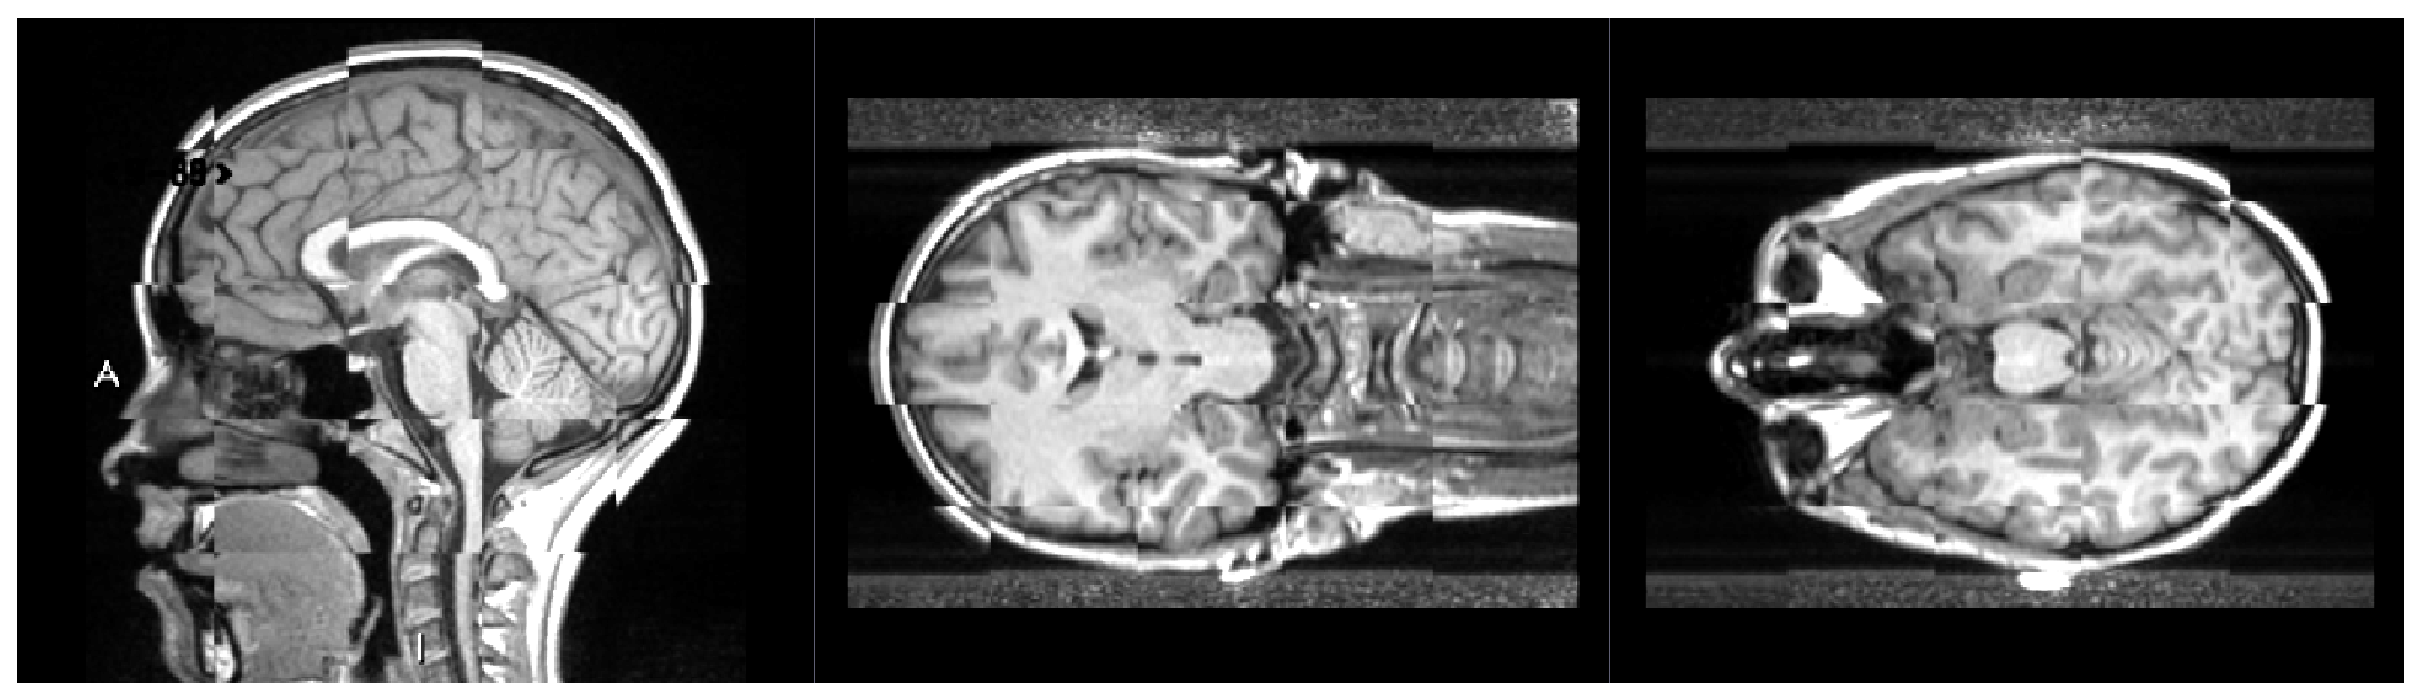
\includegraphics[scale=0.3]{before_registration.eps}
  \caption{Comparison of volumes before registration}
  \label{before_reg}
\end{figure}


\begin{figure}[htb]
  \centering
  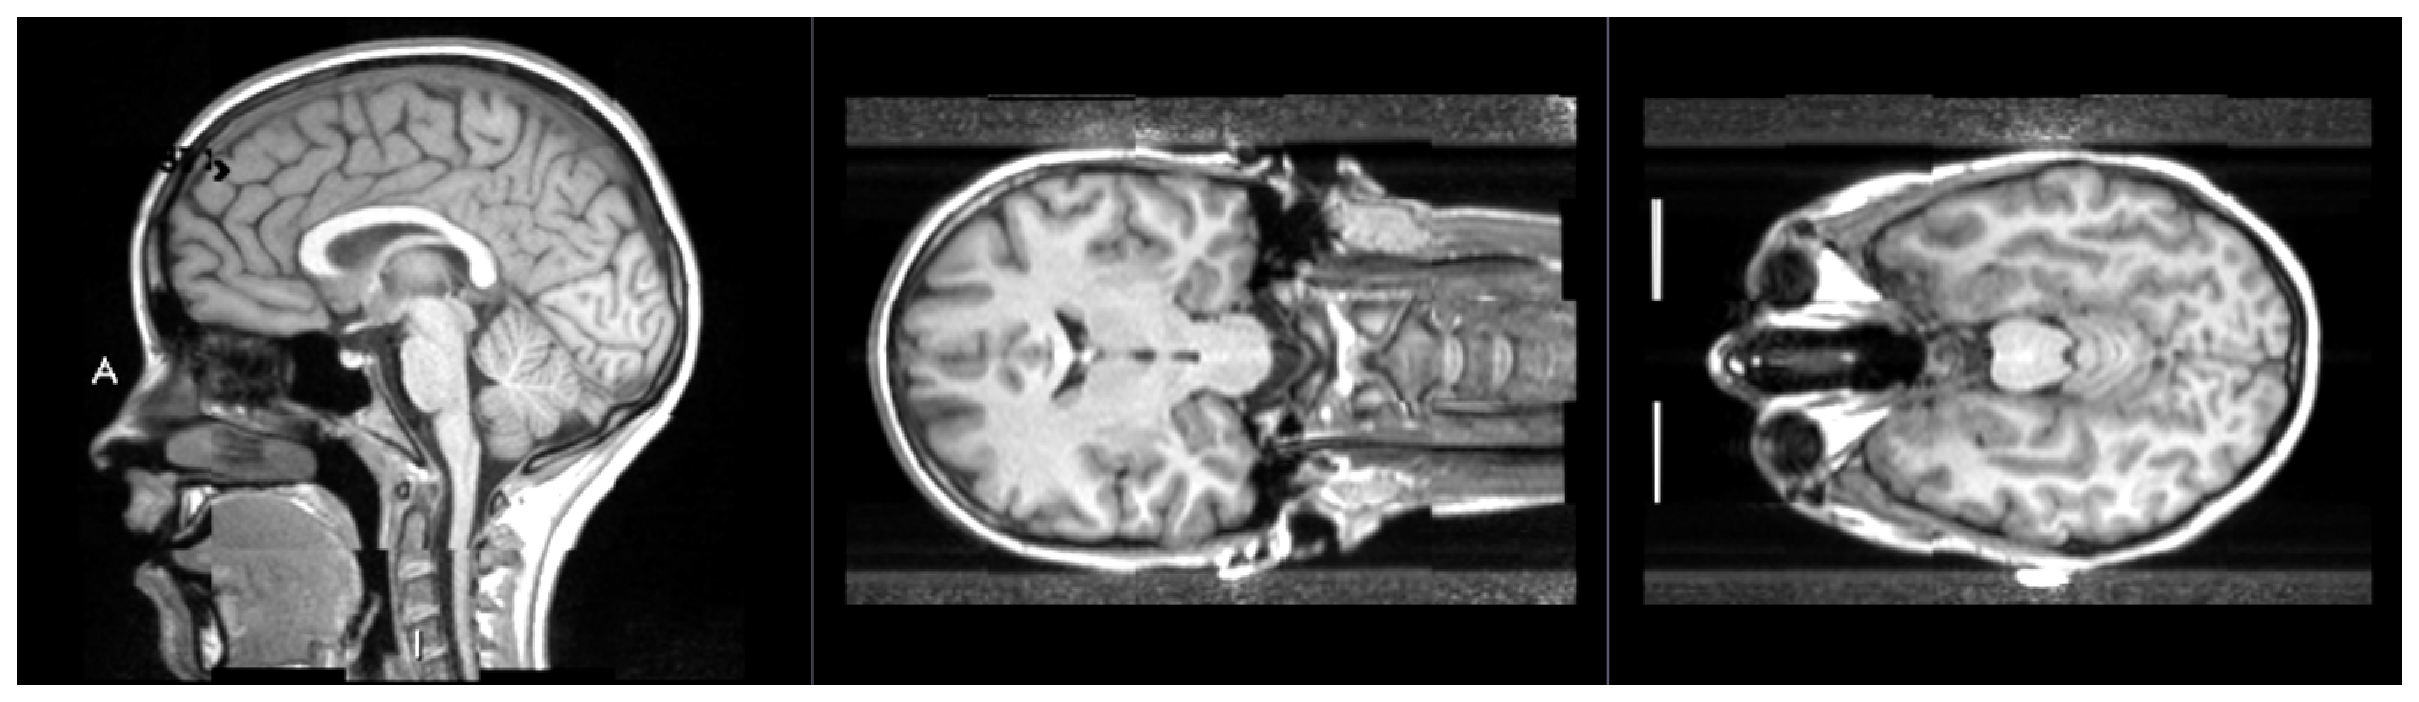
\includegraphics[scale=0.3]{after_registration.eps}
  \caption{Comparison of volumes after registration}
  \label{after_reg}
\end{figure}

The second volume has been modified using affine registration so that
the comparison between both volumes becomes much easier.\\

According to \cite{zitova}, the majority of the registration methods consist of the following steps:
\begin{enumerate}
\item \textit{Feature detection:} Salient and distinctive objects are detected.
\item \textit{Feature matching:} The correspondence between the features detected in the sensed image and those detected in the reference image is established.
\item \textit{Transform model estimation:} The type and parameters of the mapping functions are estimated. These functions align the sensed image with the reference image.
\item \textit{Image resampling and transformation:} The sensed image is transformed by means of the mapping functions.
\end{enumerate}


\subsection{Registration Methods used}
There are many different methods to accomplish registration between
images or volumes. In this project only a few of these methods were
used based on experiments performed with some of the available
methods. The chosen procedures were the ones that behaved better
under the specific conditions of this work.


\subsubsection{Affine Registration}
In geometry, an \textit{affine transformation} or an \textit{affinity}
is a transformation which preserves straight lines (i.e., all points
lying on a line initially still lie on a line after the
transformation) and ratios of distances between points lying on a
straight line. It does not necessarily preserve angles or lengths, but
does have the property that sets of parallel lines will remain
parallel to each other after an affine transformation \cite{affine_t}. \\

The implementation of affine registration used during this project is
the one included in \textit{3D Slicer} version 4.1. 

The application is able to register two images together using an
affine transform and mutual information, and it allows the user to
modify quite a few parameters
in order to obtain the expected result.\\

If you would like to know more about this implementation of affine
registration please refer to the module webpage:

\url{http://wiki.slicer.org/slicerWiki/index.php/Documentation/4.1/Modules/AffineRegistration}

\subsubsection{B-Spline Registration}
In the mathematical subfield of numerical analysis, a
\textit{B-spline} is a spline function that has minimal support with
respect to a given degree, smoothness, and domain partition.

However, in computer graphics, the term \textit{B-spline} frequently
refers to a spline curve parametrized by spline functions that are
expressed as linear combinations of \textit{B-splines} (in the
mathematical sense explained above) \cite{bspline}.\\

Just like in the case of affine registration, the implementation of
B-Spline registration used during this project is the one included in
\textit{3D Slicer} version 4.1. 

The application divides the volumes into a grid of user-defined size
in which each line is a B-spline that will be modified by the
registration to create a transform that aligns the two volumes.\\

If you would like to know more about this implementation of B-spline
registration please refer to the module webpage:

\url{http://wiki.slicer.org/slicerWiki/index.php/Documentation/4.1/Modules/BSplineDeformableRegistration}


\subsubsection{BRAINS Demon Warp Registration}
As with the registration methods explained before, \textit{BRAINS
  Demon Warp} registration is implemented as a module in \textit{3D
  Slicer} version
4.1.\\

The module works by using the ITK filter based on Thirion's Demons
algorithm, in which the main idea is to consider the objects
boundaries in one image as semi-permeable membranes and to let the
other image, considered as a deformable grid model, diffuse through
these interfaces, by the action of effectors situated within the
membranes. \cite{thirion}.

An important characteristic of this implementation, that was
particularly useful for this project, is that it can produce a
\textit{deformation field} as the output of the registration. A
deformation field is a vector image in which each point is a vector
that indicates the amount of deformation necessary
at that point in order to align the volumes.\\


If you would like to know more about the implementation of
\textit{BRAINS Demon Warp} registration please refer to the module
webpage:

\url{http://wiki.slicer.org/slicerWiki/index.php/Documentation/4.1/Modules/BRAINSDemonWarp}


\section{Morphometry}
Morphometry refers to the measurement of external form. More
specifically, \textit{brain morphometry} is concerned with the
measurement of brain structures and changes thereof during
development, aging, learning, disease and evolution. Its goal is to
derive specific information from noninvasive neuroimaging data of live
brains, typically obtained from magnetic resonance imaging (MRI); and
to quantify the anatomical features of the brain in terms of shape,
mass and volume \cite{brmorph}.

\subsection{Voxel-based Morphometry}

\subsection{Tensor-based Morphometry}
\subsection{Deformation-based Morphometry}
     \chapter{Proposed Solutions}

\section{Tools used}
\subsection{3D Slicer}
\textbf{Slicer}, or \textbf{3D Slicer}, is a free, open source software package for visualization and image analysis. It is natively designed to be available on multiple platforms, including Windows, Linux and Mac Os X.

3D Slicer provides image registration, processing of DTI (diffusion tractography), an interface to external devices for image guidance support, and GPU-enabled volume rendering, among other capabilities. 3D Slicer has a modular organization that allows the easy addition of new functionality and provides a number of generic features not available in competing tools.

3D Slicer is built on VTK, a pipeline-based graphical library that is widely used in scientific visualization. In version 4, the core application is implemented in C++, and the API is available through a Python wrapper to facilitate rapid, iterative development and visualization in the included Python console. The user interface is implemented in Qt, and may be extended using either C++ or Python.

Slicer supports several types of modular development. Fully interactive, custom interfaces may be written in C++ or Python. Command-line programs in any language may be wrapped using a light-weight XML specification, from which a graphical interface is automatically generated \cite{slicer}.

For more information on this tool please refer to its official webpage: 

\url{http://www.slicer.org/}

\subsection{ITK}
ITK stands for \textbf{Insight Segmentation and Registration Toolkit}, it's a cross-platform, open-source application development framework widely used for the development of image segmentation and image registration programs.

ITK  is implemented in C++ and it is wrapped for Tcl, Python and Java. This enables developers to create software using a variety of programming languages.

ITK's code is highly efficient, which means that many software problems are discovered at compile-time, rather than at run-time during program execution. It also enables ITK to work on two, three, four or more dimensions.

For more information on this tool please refer to its official webpage: 

\url{http://www.itk.org/}

\subsection{Other Tools}
\subsubsection{Programming Languages}
The programming languages chosen during this project are \textbf{C++} and \textbf{Python}, mainly because they are main languages in which 3D Slicer is written, which means that it was easier to communicate with 3D Slicer by using them.

\subsubsection{MATLAB}
MATLAB is a numerical computing environment and programming language. It allows matrix manipulations, plotting of functions and data, implementation of algorithms, creation of user interfaces, and interfacing with programs written in other languages, including C, C++, Java, and Fortran \cite{matlab}.

MATLAB was used during this project specifically to create and quickly manipulate MRI volume files.

Official website for this tool: \url{http://www.mathworks.com/}

\subsubsection{ParaView}
ParaView is an open-source, multi-platform data analysis and visualization application. ParaView users can quickly build visualizations to analyze their data using qualitative and quantitative techniques.

ParaView was used during this project to visualize the deformation fields produced after the registration of two volumes.

Official website for this tool: \url{http://www.paraview.org/}

\section{Implemented Methods}
During the course of this project two different methods where
implemented, both taking into account previous works about morphometry
and quantification of small changes in volumes.

\subsection{Voxel-based method}
This method was implemented as a \textit{3D Slicer} module with the following steps:
\begin{enumerate}
\item The user selects the base and follow-up volumes to be compared.
\item The user selects the registration method to be used and applies it on the volumes.
\item The module subtracts the base volume and the volume resulting
  from the registration and shows the resulting differences as colored
  layer on top of the base volume.
\end{enumerate}

The registration methods available are: \textit{Affine registration}
(default), \textit{B-Spline deformable registration} and
\textit{BRAINS Demon Warp registration}; all of them available as
already existing modules in \textit{3D Slicer}.

For more information on the registration methods, please refer to
section~\ref{sec:reg_methods}.\\

The subtraction is done pixel-by-pixel and the result produces a label
volume that shows the differences in color over the original base
volume. The chosen color table for the label volume is ``PET-Heat'',
directly available in \textit{3D Slicer}, since it seemed to produce a
volume that was brighter and with easier to spot differences.

\subsubsection{Example}
The following is an example of a volume without mayor differences that
has been modified in order to add some obvious differences in the
shape of circles in both of the original volumes. 

A real user of the application would go through the following steps:

\begin{enumerate}
\item The user selects the \textit{MRIChangeDetectorModule} in \textit{3D Slicer}.

  \begin{figure}[H]
    \centering
    \includegraphics[scale=0.2]{/voxel_example/0.Select.eps}
    \caption{Step 0: Module selection}
    \label{voxel_ex_0}
  \end{figure}
  
\item The user adds the volumes to be analysed.
  
  \begin{figure}[H]
    \centering
    \includegraphics[scale=0.2]{/voxel_example/1.Volumes.eps}
    \caption{Step 1: Adding volumes}
    \label{voxel_ex_1}
  \end{figure}
  
\item The user chooses the registration method to be applied.
  
  \begin{figure}[H]
    \centering
    \includegraphics[scale=0.2]{/voxel_example/2.Registration.eps}
    \caption{Step 2: Registration method}
    \label{voxel_ex_2}
  \end{figure}
  
  
\item The user clicks the button ``Run Quantification'' and the
  program runs the subtraction and creation of label volume.
  
  \begin{figure}[H]
    \centering
    \includegraphics[scale=0.2]{/voxel_example/3.Quantification.eps}
    \caption{Step 3: Running quantification}
    \label{voxel_ex_3}
  \end{figure}
  
\item The program shows the resulting label volume.
  
  \begin{figure}[H]
    \centering
    \includegraphics[scale=0.2]{/voxel_example/4.Result1.eps}
    \caption{Step 4: Quantification result}
    \label{voxel_ex_4}
  \end{figure}

  Note that the resulting differences look like rings. This is the
  expected result because both of the original volumes were modified
  by adding circles of distinct sizes.
  
\item The user can now watch the label volume on top of the original
  volume and move the planes as he wishes.
  
  \begin{figure}[H]
    \centering
    \includegraphics[scale=0.2]{/voxel_example/5.Result2.eps}
    \caption{Step 5: User visualization}
    \label{voxel_ex_5}
  \end{figure}

\end{enumerate}


\subsubsection{Technical Details}
The user interface of the module is written in \textit{Python} using
some libraries from \textit{Qt} and \textit{CTK}, being
\textit{ctkWorkflowWidgetStep} from \textit{CTK} the most important
since it allows the creation of a ``step-by-step'' wizard.\\


The part of the module in charge of the subtraction of volumes is
written in \textit{C++} using \textit{ITK}.

The subtraction is done using the ITK filter
\textit{AbsoluteValueDifferenceImageFilter}, which computes the
difference between each two pixels and then calculates the absolute
value of the result. This allows the module to detect all the possible
differences between the volumes, regardless of the sign of the
resulting values.\\


\subsection{Tensor-based method}
This method was also implemented as a \textit{3D Slicer} module with the following steps:
\begin{enumerate}
\item The user selects the base and follow-up volumes to be compared.
\item The user selects the displacement field smoothing sigma to use during the registration and runs it.
\item The user selects the percentage of growth and shrinkage that he
  would like to see and runs the measurements. The module shows the
  result as a colored layer on top of the base volume.
\end{enumerate}

The registration method that is used in this case is \textit{BRAINS
  Demon Warp Registration}, for more information on this method please
refer to section \ref{sec:demon_warp}.\\

The \textit{displacement field smoothing sigma} is a Gaussian
smoothing value to be applied to the output deformation field at each
iteration of the registration process. Increasing this value produces
deformation fields that are smoother and where the vector values are
less prone to show big changes over very small movements in the field.

The default value for the smoothing sigma is $1.0$; however, according
to our experiments, to produce deformation fields that are smooth
enough the value should be between $2.0$ and $3.0$.\\

The module also allows the user to choose the percentage of the values
of the \textit{Jacobian determinants} that will be shown in the final
result. Since there are two types of values (corresponding to growing
and shrinking of the original volume), there is also two values to
select. For example, if the user chooses to view $50\%$ of the growth
values, only half of the values that represent growth in the
deformation field will actually be shown on the resulting label map.\\
% TODO something about which values are better?

Once the user has seen the results with certain percentages, the
module can be run again with a new set of parameters in order to get
better results.

\subsubsection{Example}
The tensor-based method will be applied to the same volumes used in
the previous example. A real user of the application would go through
the following steps:

\begin{enumerate}
\item The user selects the \textit{TensorMRIChangeDetectorModule} in \textit{3D Slicer}.

  \begin{figure}[H]
    \centering
    \includegraphics[scale=0.2]{/tensor_example/0.Select.eps}
    \caption{Step 0: Module selection}
    \label{tensor_ex_0}
  \end{figure}
  
\item The user adds the volumes to be analysed.
  
  \begin{figure}[H]
    \centering
    \includegraphics[scale=0.2]{/tensor_example/1.Volumes.eps}
    \caption{Step 1: Adding volumes}
    \label{tensor_ex_1}
  \end{figure}
  
\item The user chooses the deformation field smoothing sigma and begins the registration. 
  
  \begin{figure}[H]
    \centering
    \includegraphics[scale=0.2]{/tensor_example/2.Registration.eps}
    \caption{Step 2: DEMONS Warp Registration}
    \label{tensor_ex_2}
  \end{figure}
  
  
\item  The user chooses the percentage of growth and shrinkage to
  use in the output label map and clicks the button ``Run Tensor
  measurements'' to initiate the tensor calculations.

  \begin{figure}[H]
    \centering
    \includegraphics[scale=0.2]{/tensor_example/3.Quantification.eps}
    \caption{Step 3: Running tensor measurements}
    \label{tensor_ex_3}
  \end{figure}
  
  The volume that can be observed in the image is the deformation
  field produced by the registration from the previous step.

\item The program shows the resulting label volume directly on top of the original volume.
  
  \begin{figure}[H]
    \centering
    \includegraphics[scale=0.2]{/tensor_example/4.Result1.eps}
    \caption{Step 4: Quantification result}
    \label{tensor_ex_4}
  \end{figure}
  
\item The user can now move the planes and visualise the volumes as desired.
  
  \begin{figure}[H]
    \centering
    \includegraphics[scale=0.2]{/tensor_example/5.Result2.eps}
    \caption{Step 5: User visualization}
    \label{tensor_ex_5}
  \end{figure}


\item The user can change the percentage numbers depending on what he
  or she wants to see and re-run the module by clicking the button
  once again.
  
  \begin{figure}[H]
    \centering
    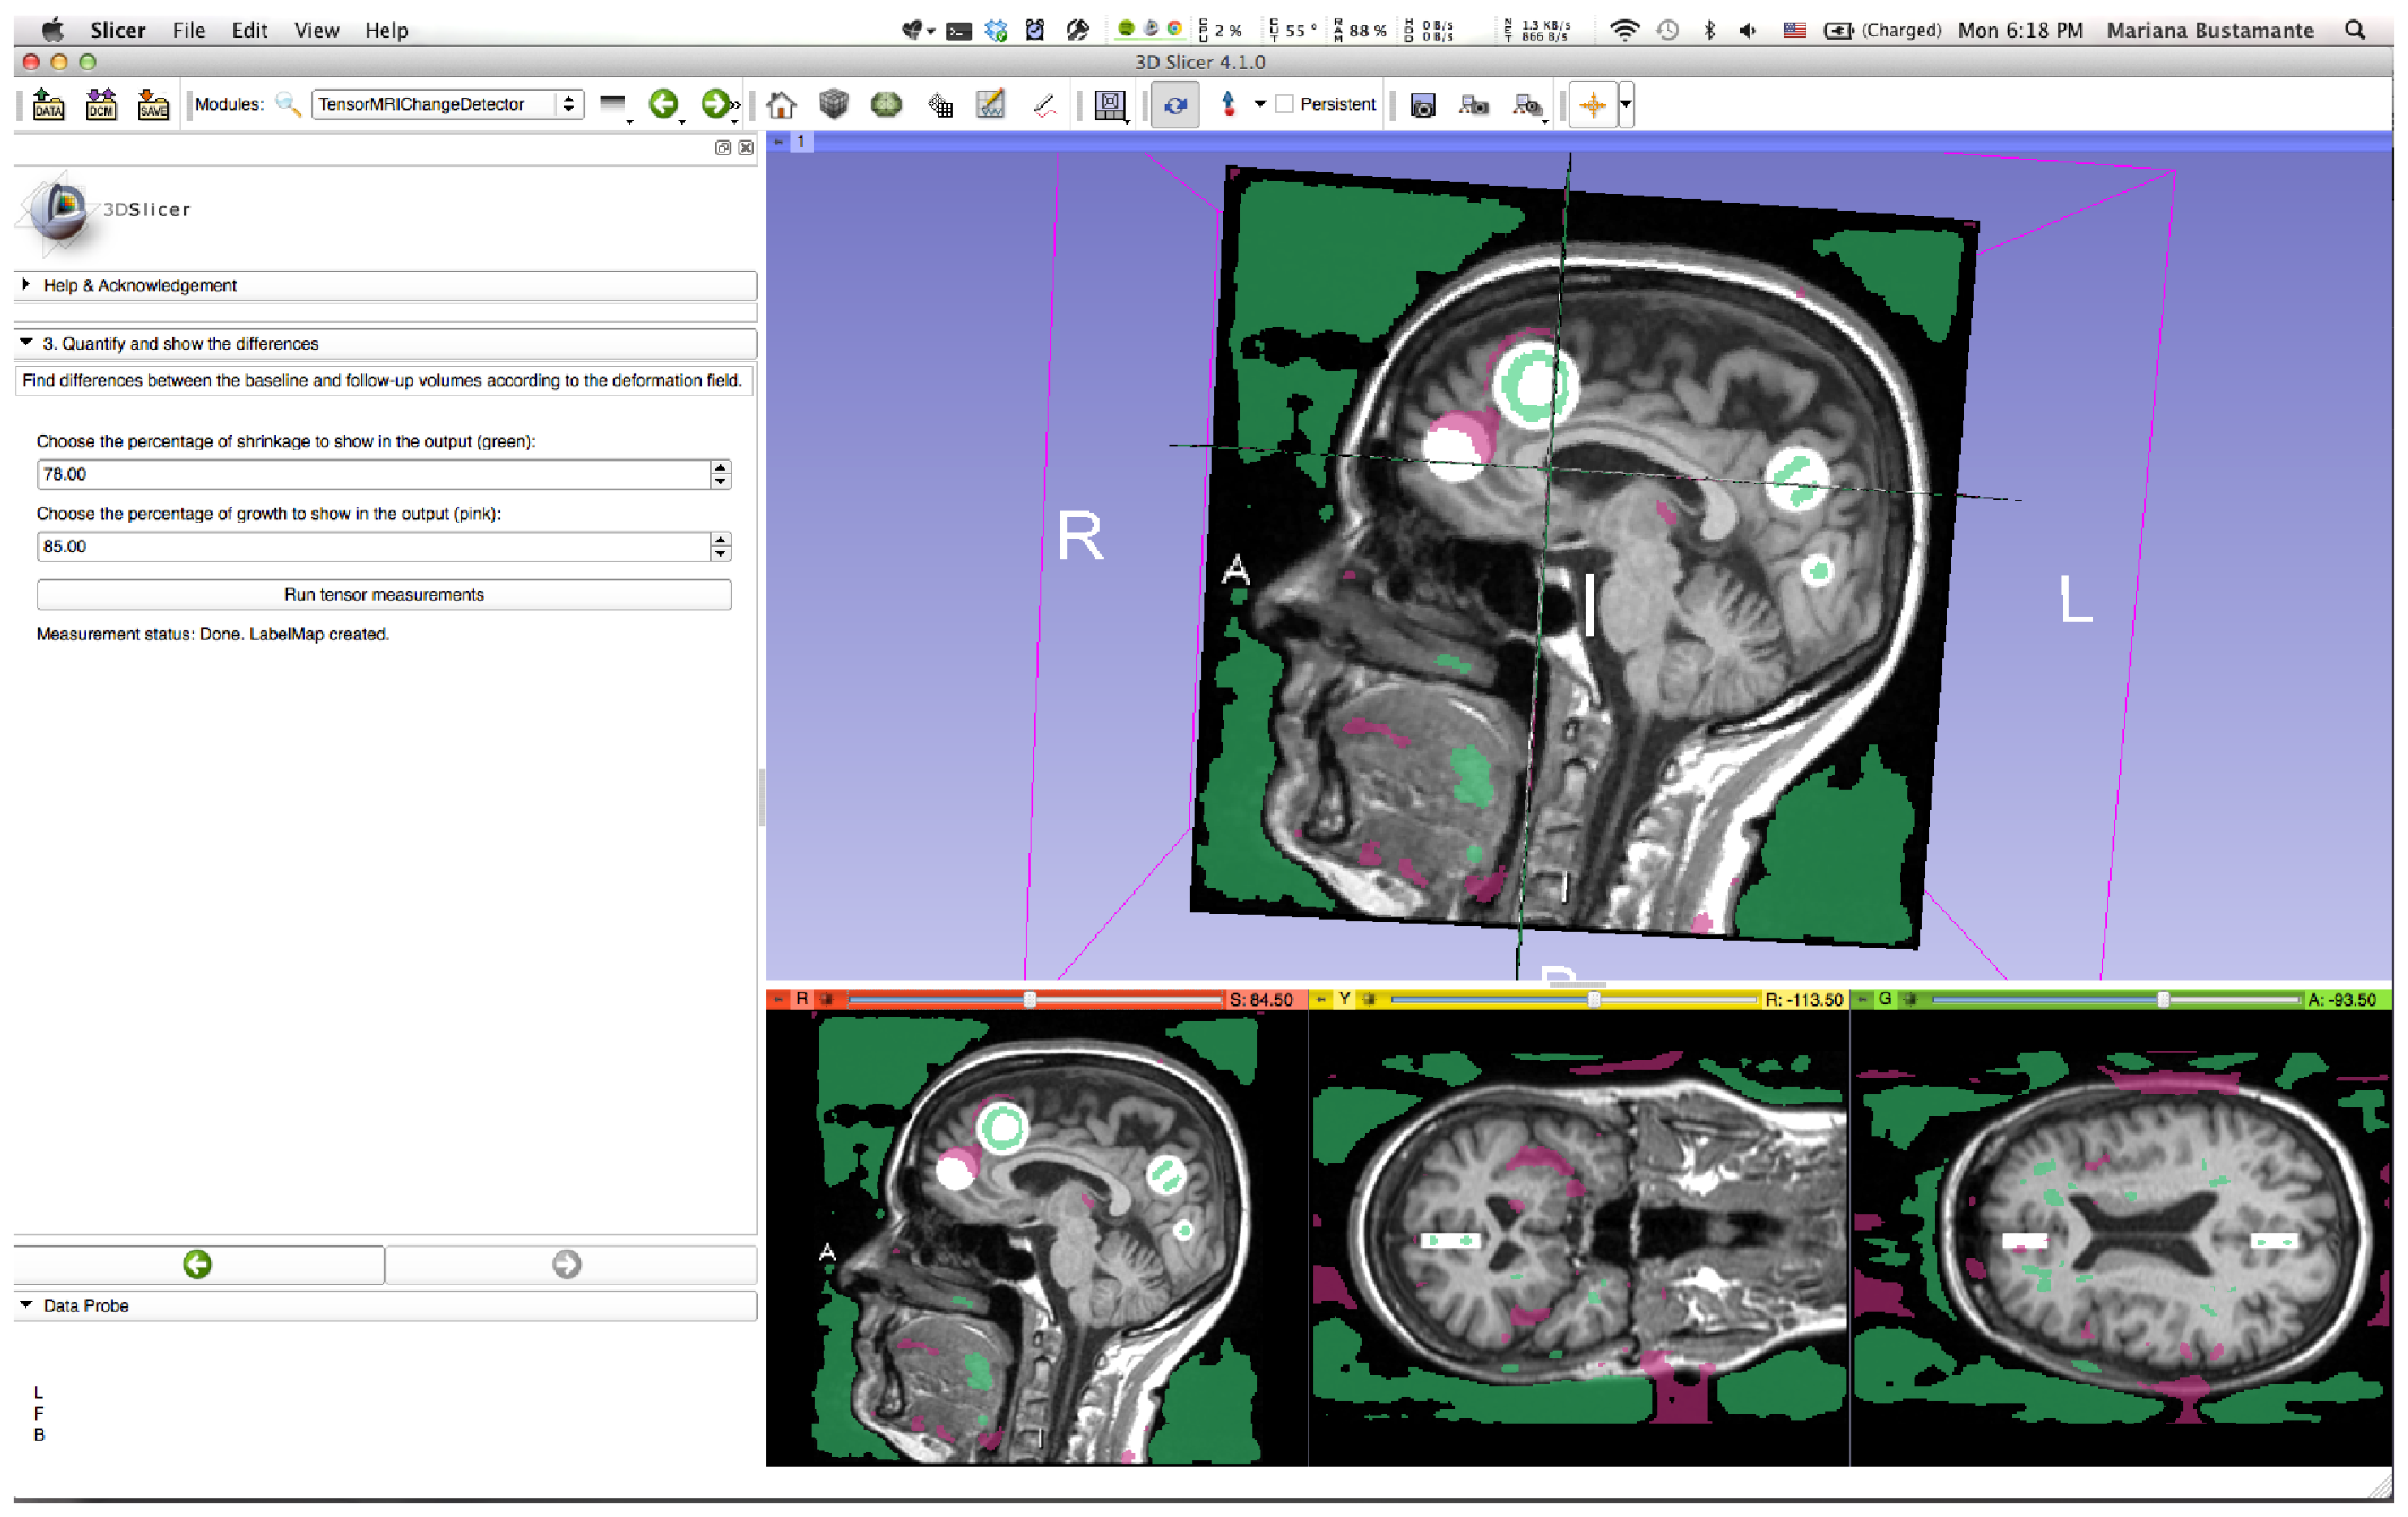
\includegraphics[scale=0.2]{/tensor_example/6.Result3.eps}
    \caption{Step 6: Interactive growth/shrinkage values}
    \label{tensor_ex_6}
  \end{figure}

\end{enumerate}


\subsubsection{Technical Details}
Like the voxel-based method, the user interface of the module is
written in \textit{Python} using some libraries from \textit{Qt} and
\textit{CTK}, being \textit{ctkWorkflowWidgetStep} from \textit{CTK}
the most important since it allows the creation of a ``step-by-step''
wizard.\\

The tensor measurements are written in \textit{C++} using
\textit{ITK}. It is the most important part of the method and it
includes the following functionalities:
\begin{itemize}
\item Computation of the \textit{Jacobian determinant} at each point
  in the deformation field by using the filter
  \textit{DisplacementFieldJacobianDeterminantFilter}.
\item Initially the Jacobian values are centered on $1.0$, this means
  that when the values are close to $1.0$ the change in the volume is
  nonexistent or small enough to be ignored. 

  In order to move the ``no-change-zone'' from $1.0$ to $0.0$, a
  \textit{logarithm} filter is applied on the Jacobian values.
  %TODO is there a better reason?
  
\item Computation of the \textit{Jacobian determinant} values that
  will be shown on the final result according to the percentages
  chosen by the user.
\item Creation of a label map with two colors that represent growth
  and shrinkage only showing the amount of values specified by the
  user.
\item Creation of a volume with all the values of the \textit{Jacobian
    determinant} for comparison with the previously described label
  map.
\end{itemize}

     \chapter{Experiments}
This section shows the results of the experiments done with the
implemented solutions. 

The methods were tried with volumes to which artificial differences of
distinct sizes and shapes were added; and also with real patient's
volumes obtained from the Uppsala University Hospital.


\section{Experiments Conditions}

\subsection{Artificial Differences}
For this experiments, the MRIs used belong to a healthy patient and
the time difference between each exam is very short, so it is expected
of them to have no changes.

The methods were used on three distinct sizes of difference: large,
medium and small. The considered sizes are based on the comparisons
done with real patients and the sizes of the differences presented on
those cases.


\subsection{Real Differences}
For this experiment, the MRIs from three real patients with known
differences were compared using both methods.

Two of them are patients of the study for which this project was
started, and so they have very small differences that are hard to
detect with the naked eye.

The third patient has larger known differences produced by a medical
condition and its subsequent surgery.


\section{Artificial Differences Results}

\subsection{Size: Large}

Initial baseline volume without modifications:

\begin{figure}[H]
  \centering
  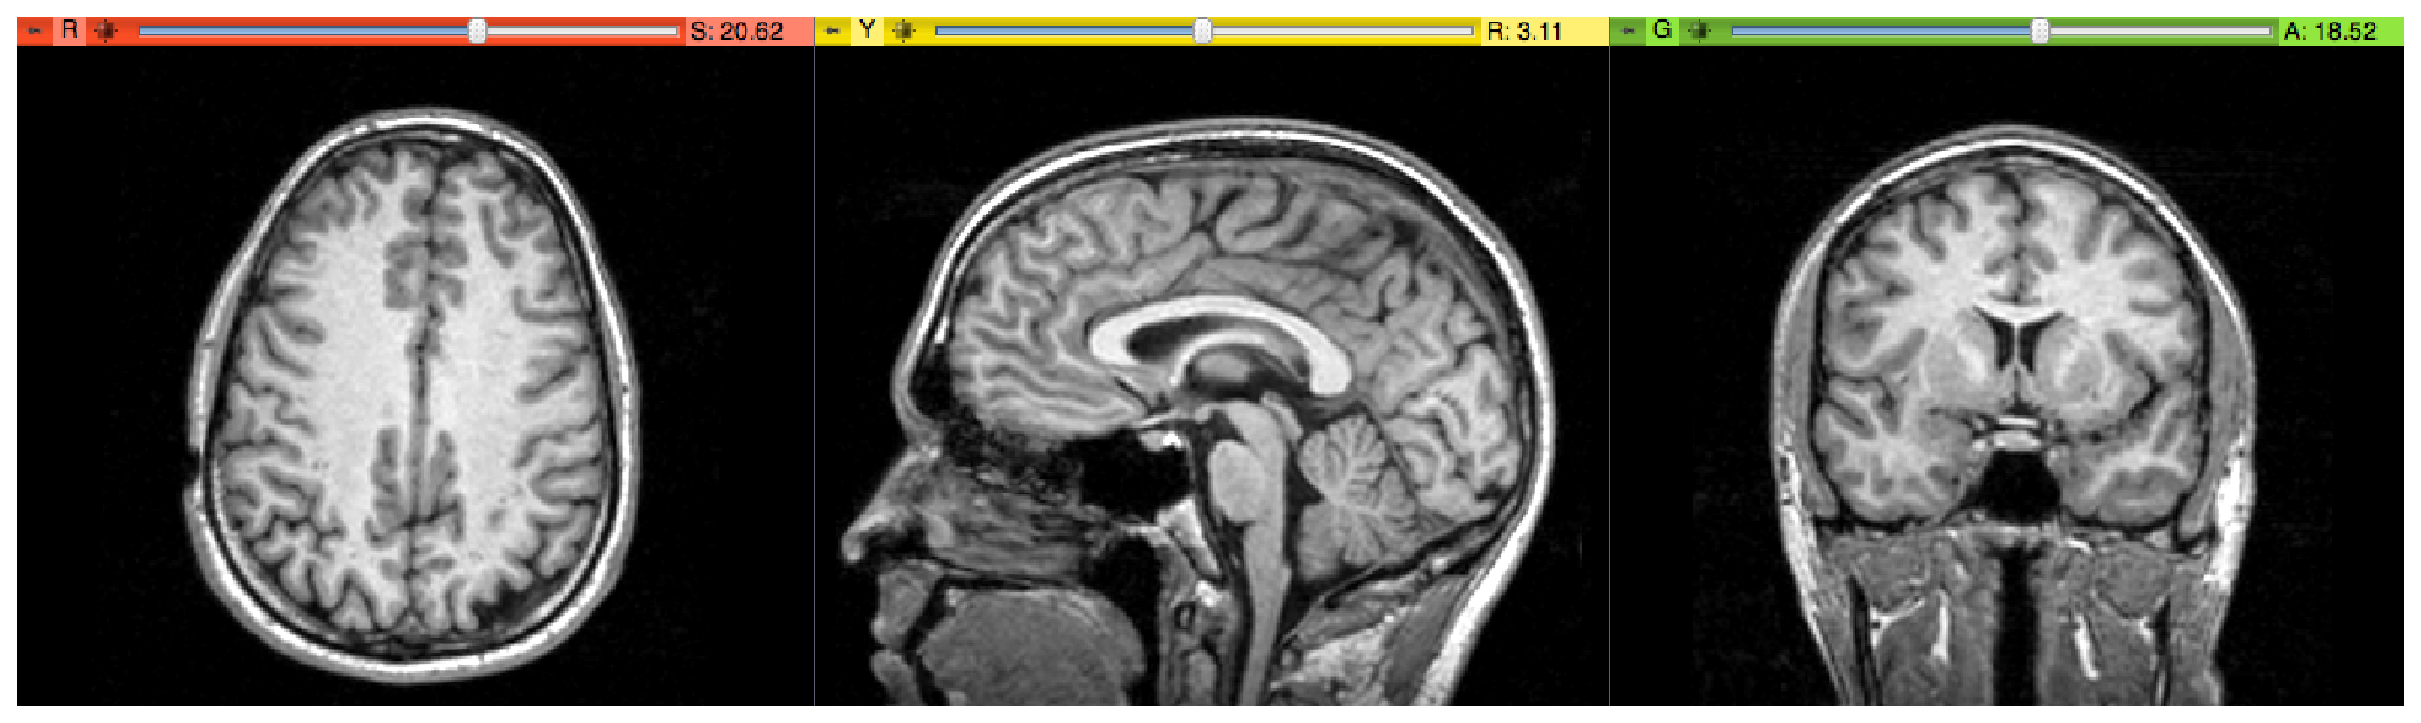
\includegraphics[scale=0.3]{/experiment_bigger/biggerA.eps}
  \caption{Large Differences: Baseline volume}
  \label{largeA}
\end{figure}

Cubes of large size where deleted from the follow-up volume to
represent areas of volume loss. The following volume was obtained:

\begin{figure}[H]
  \centering
  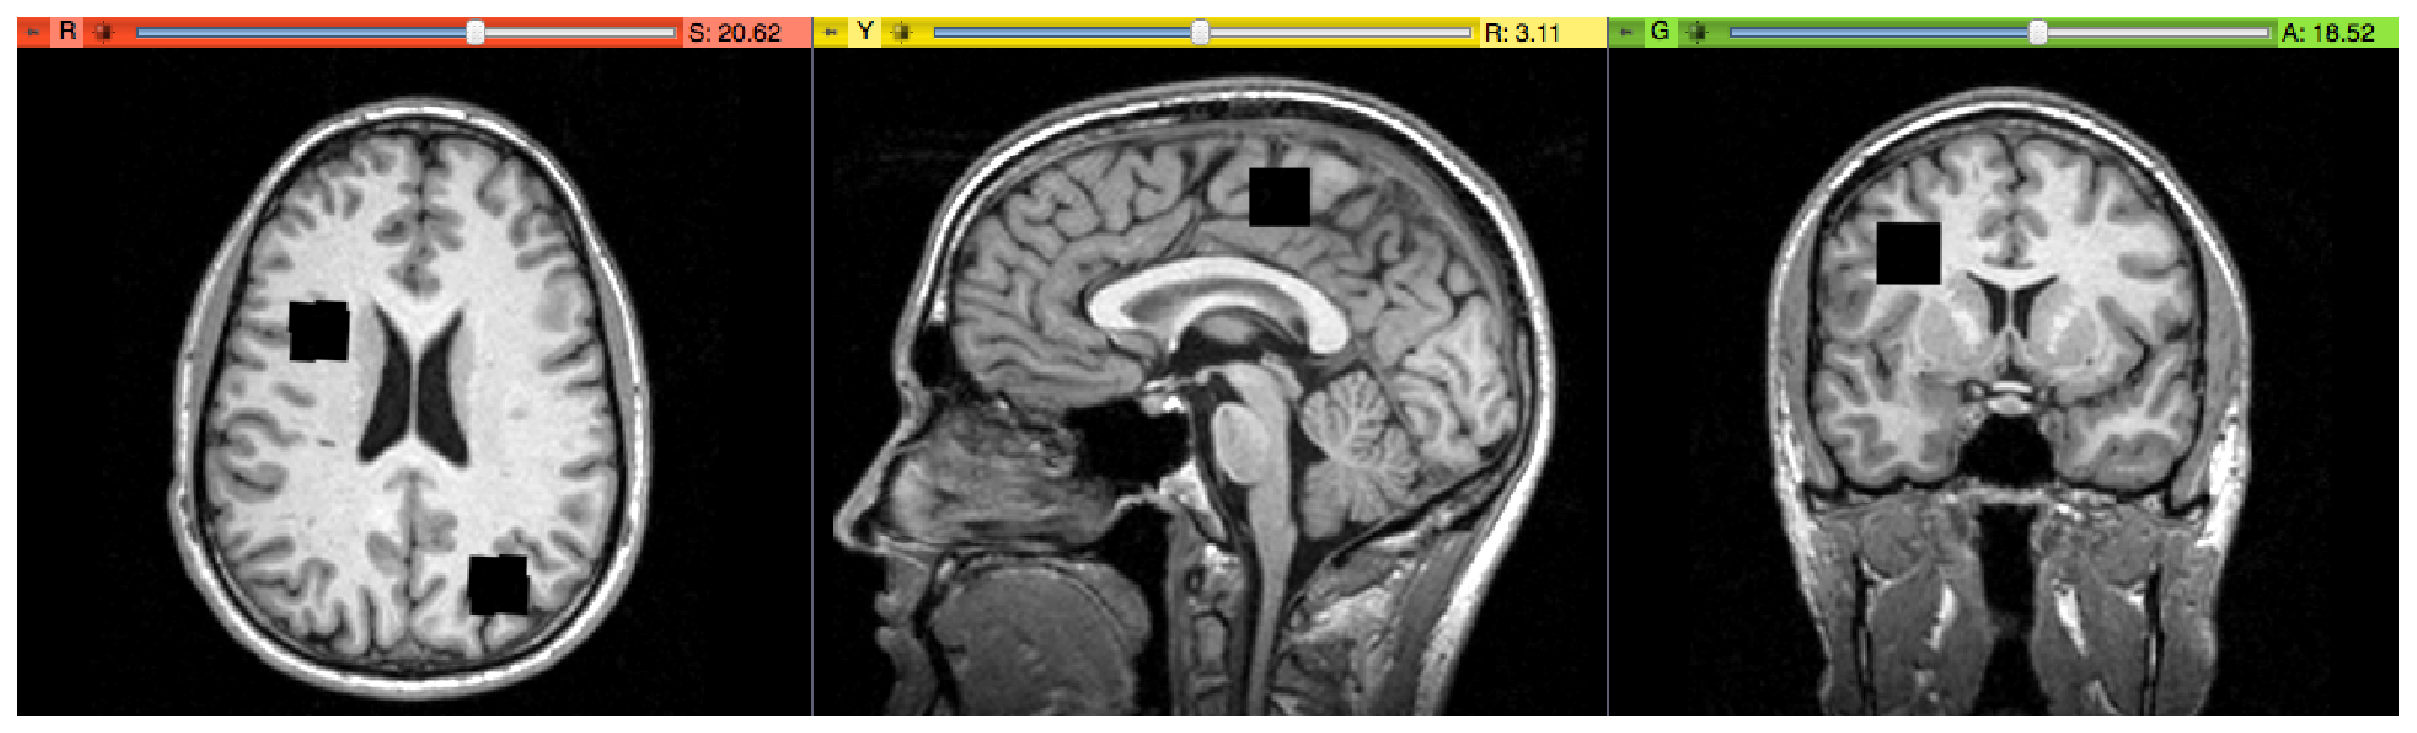
\includegraphics[scale=0.3]{/experiment_bigger/biggerB_subtracted.eps}
  \caption{Large Differences: Modified Follow-up volume}
  \label{largeB}
\end{figure}

\subsubsection{Voxel-based Method}
The result obtained with this method and large differences is pretty
good. All the differences are found and easy to see in the result.

\begin{figure}[H]
  \centering
  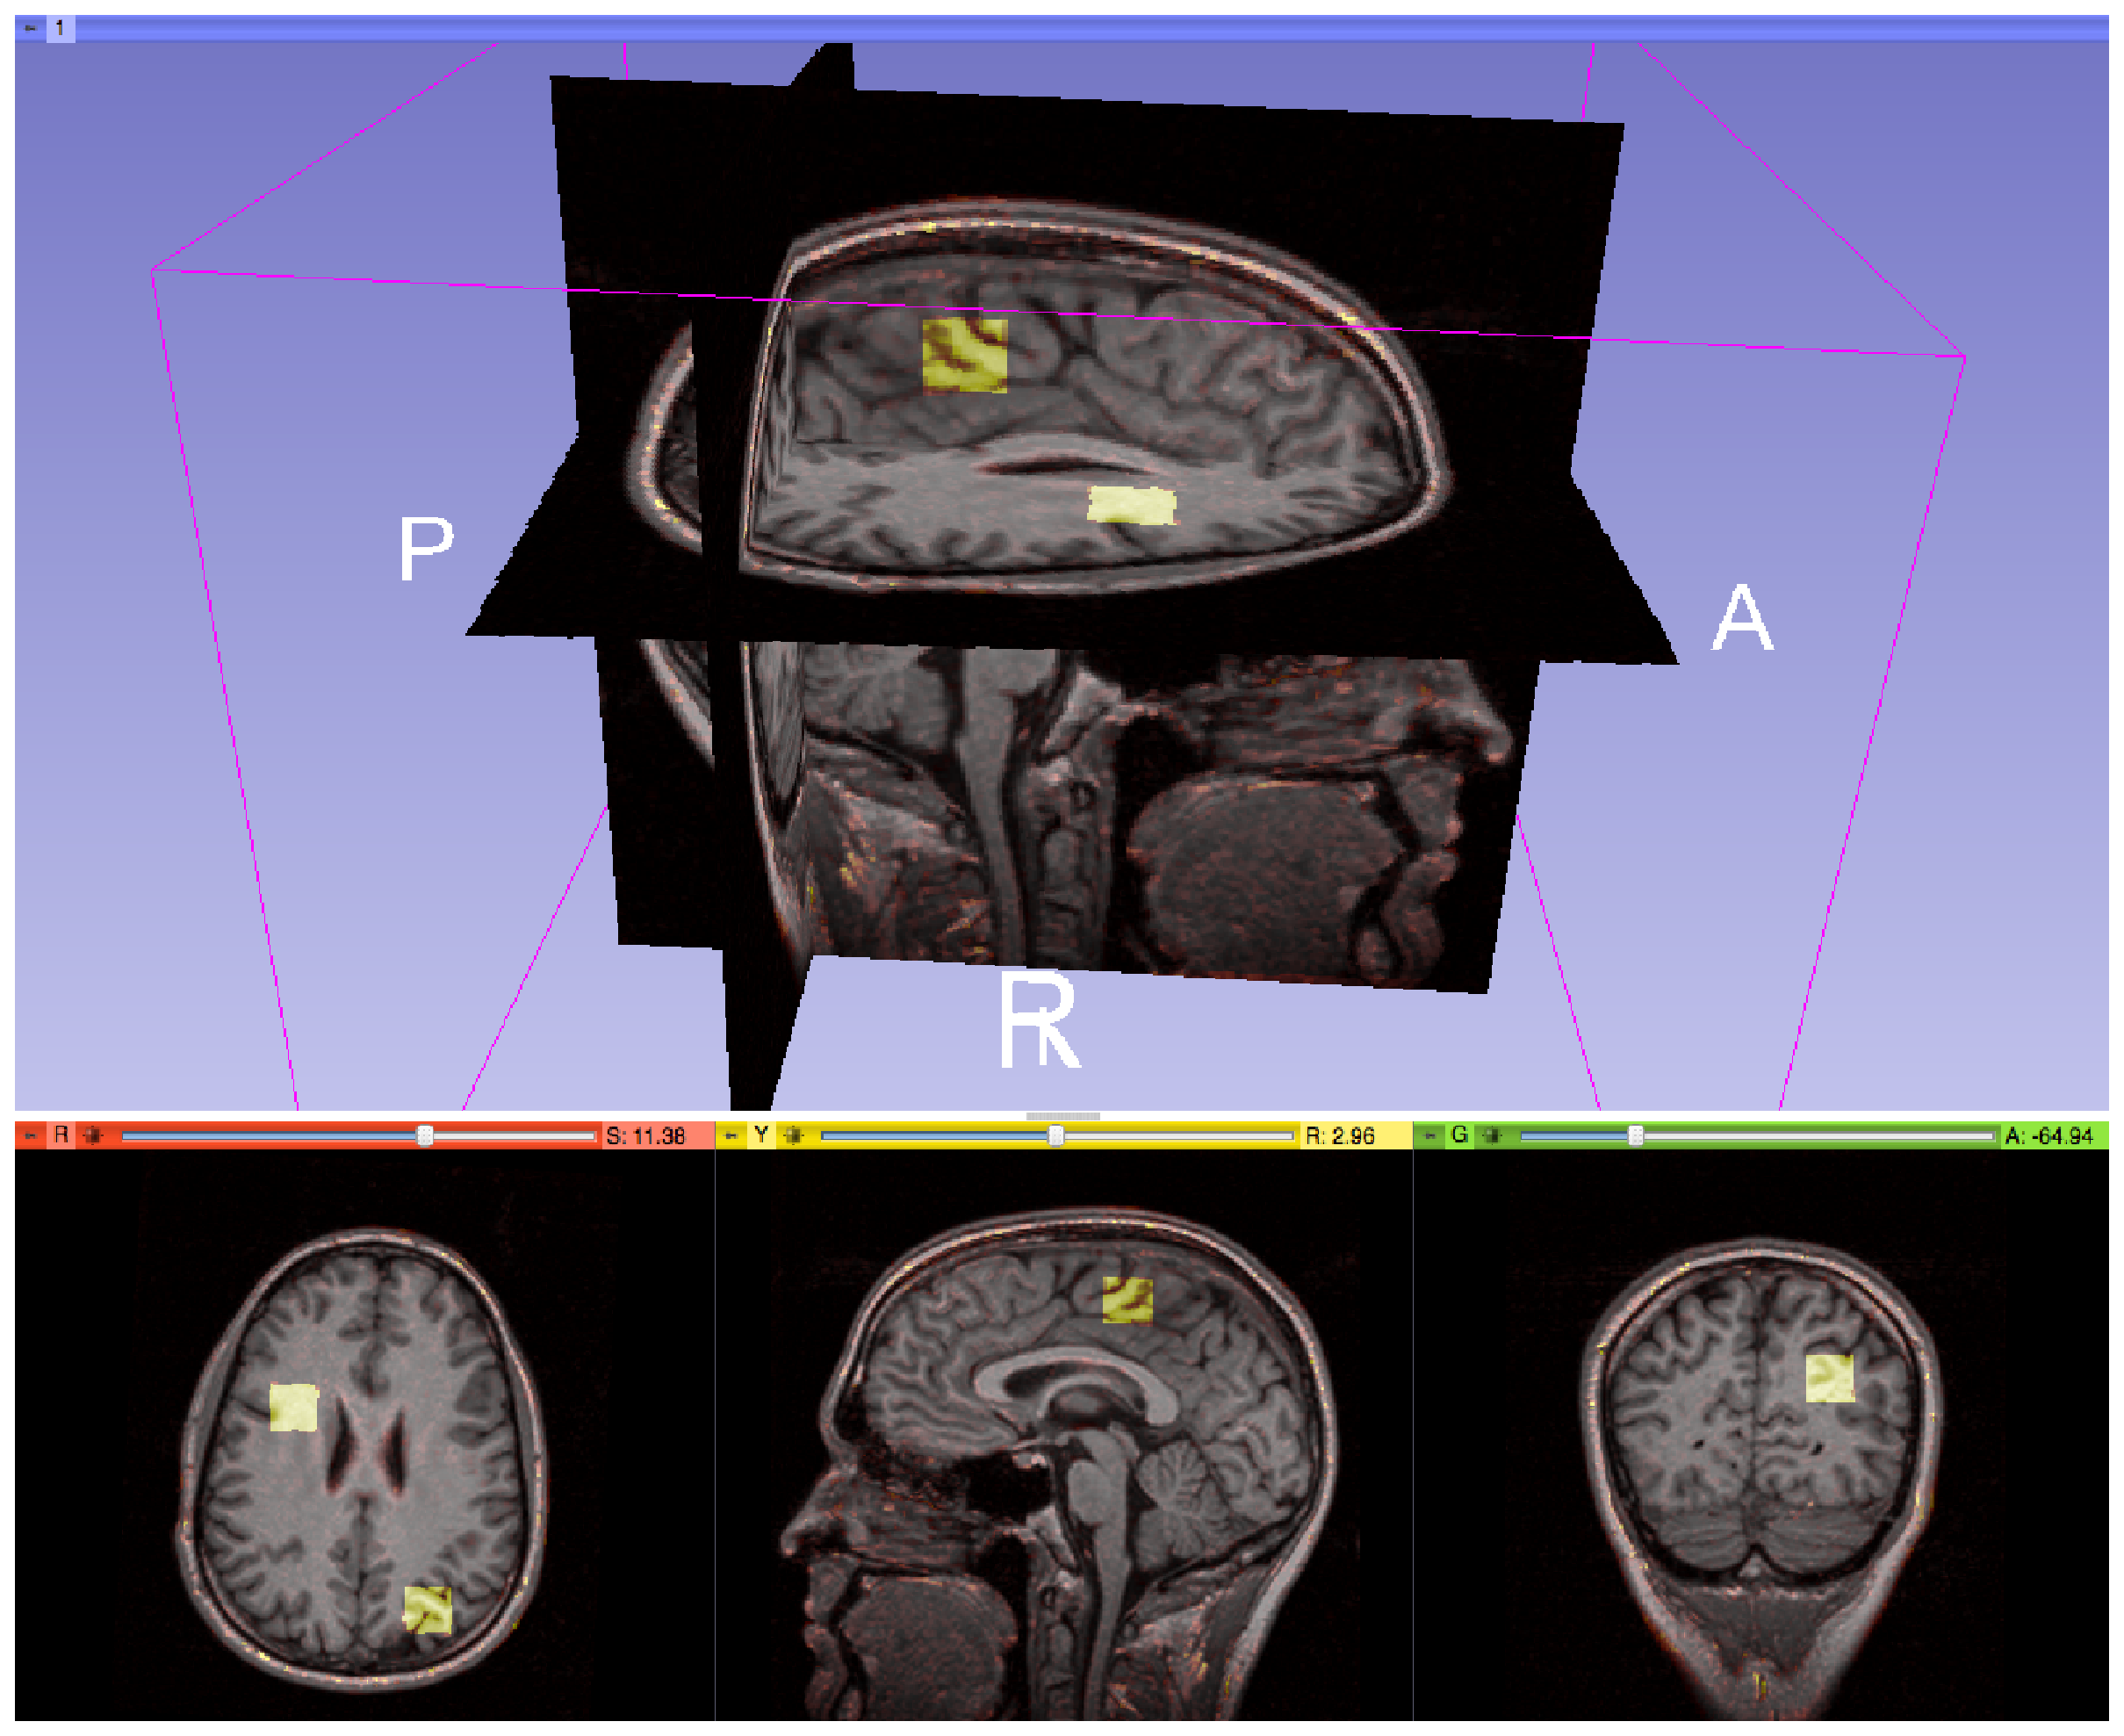
\includegraphics[scale=0.2]{/experiment_bigger/voxel_bigger1.eps}
  \caption{Artificial Large: Voxel-base method}
  \label{voxel_large1}
\end{figure}

Another angle of the result:

\begin{figure}[H]
  \centering
  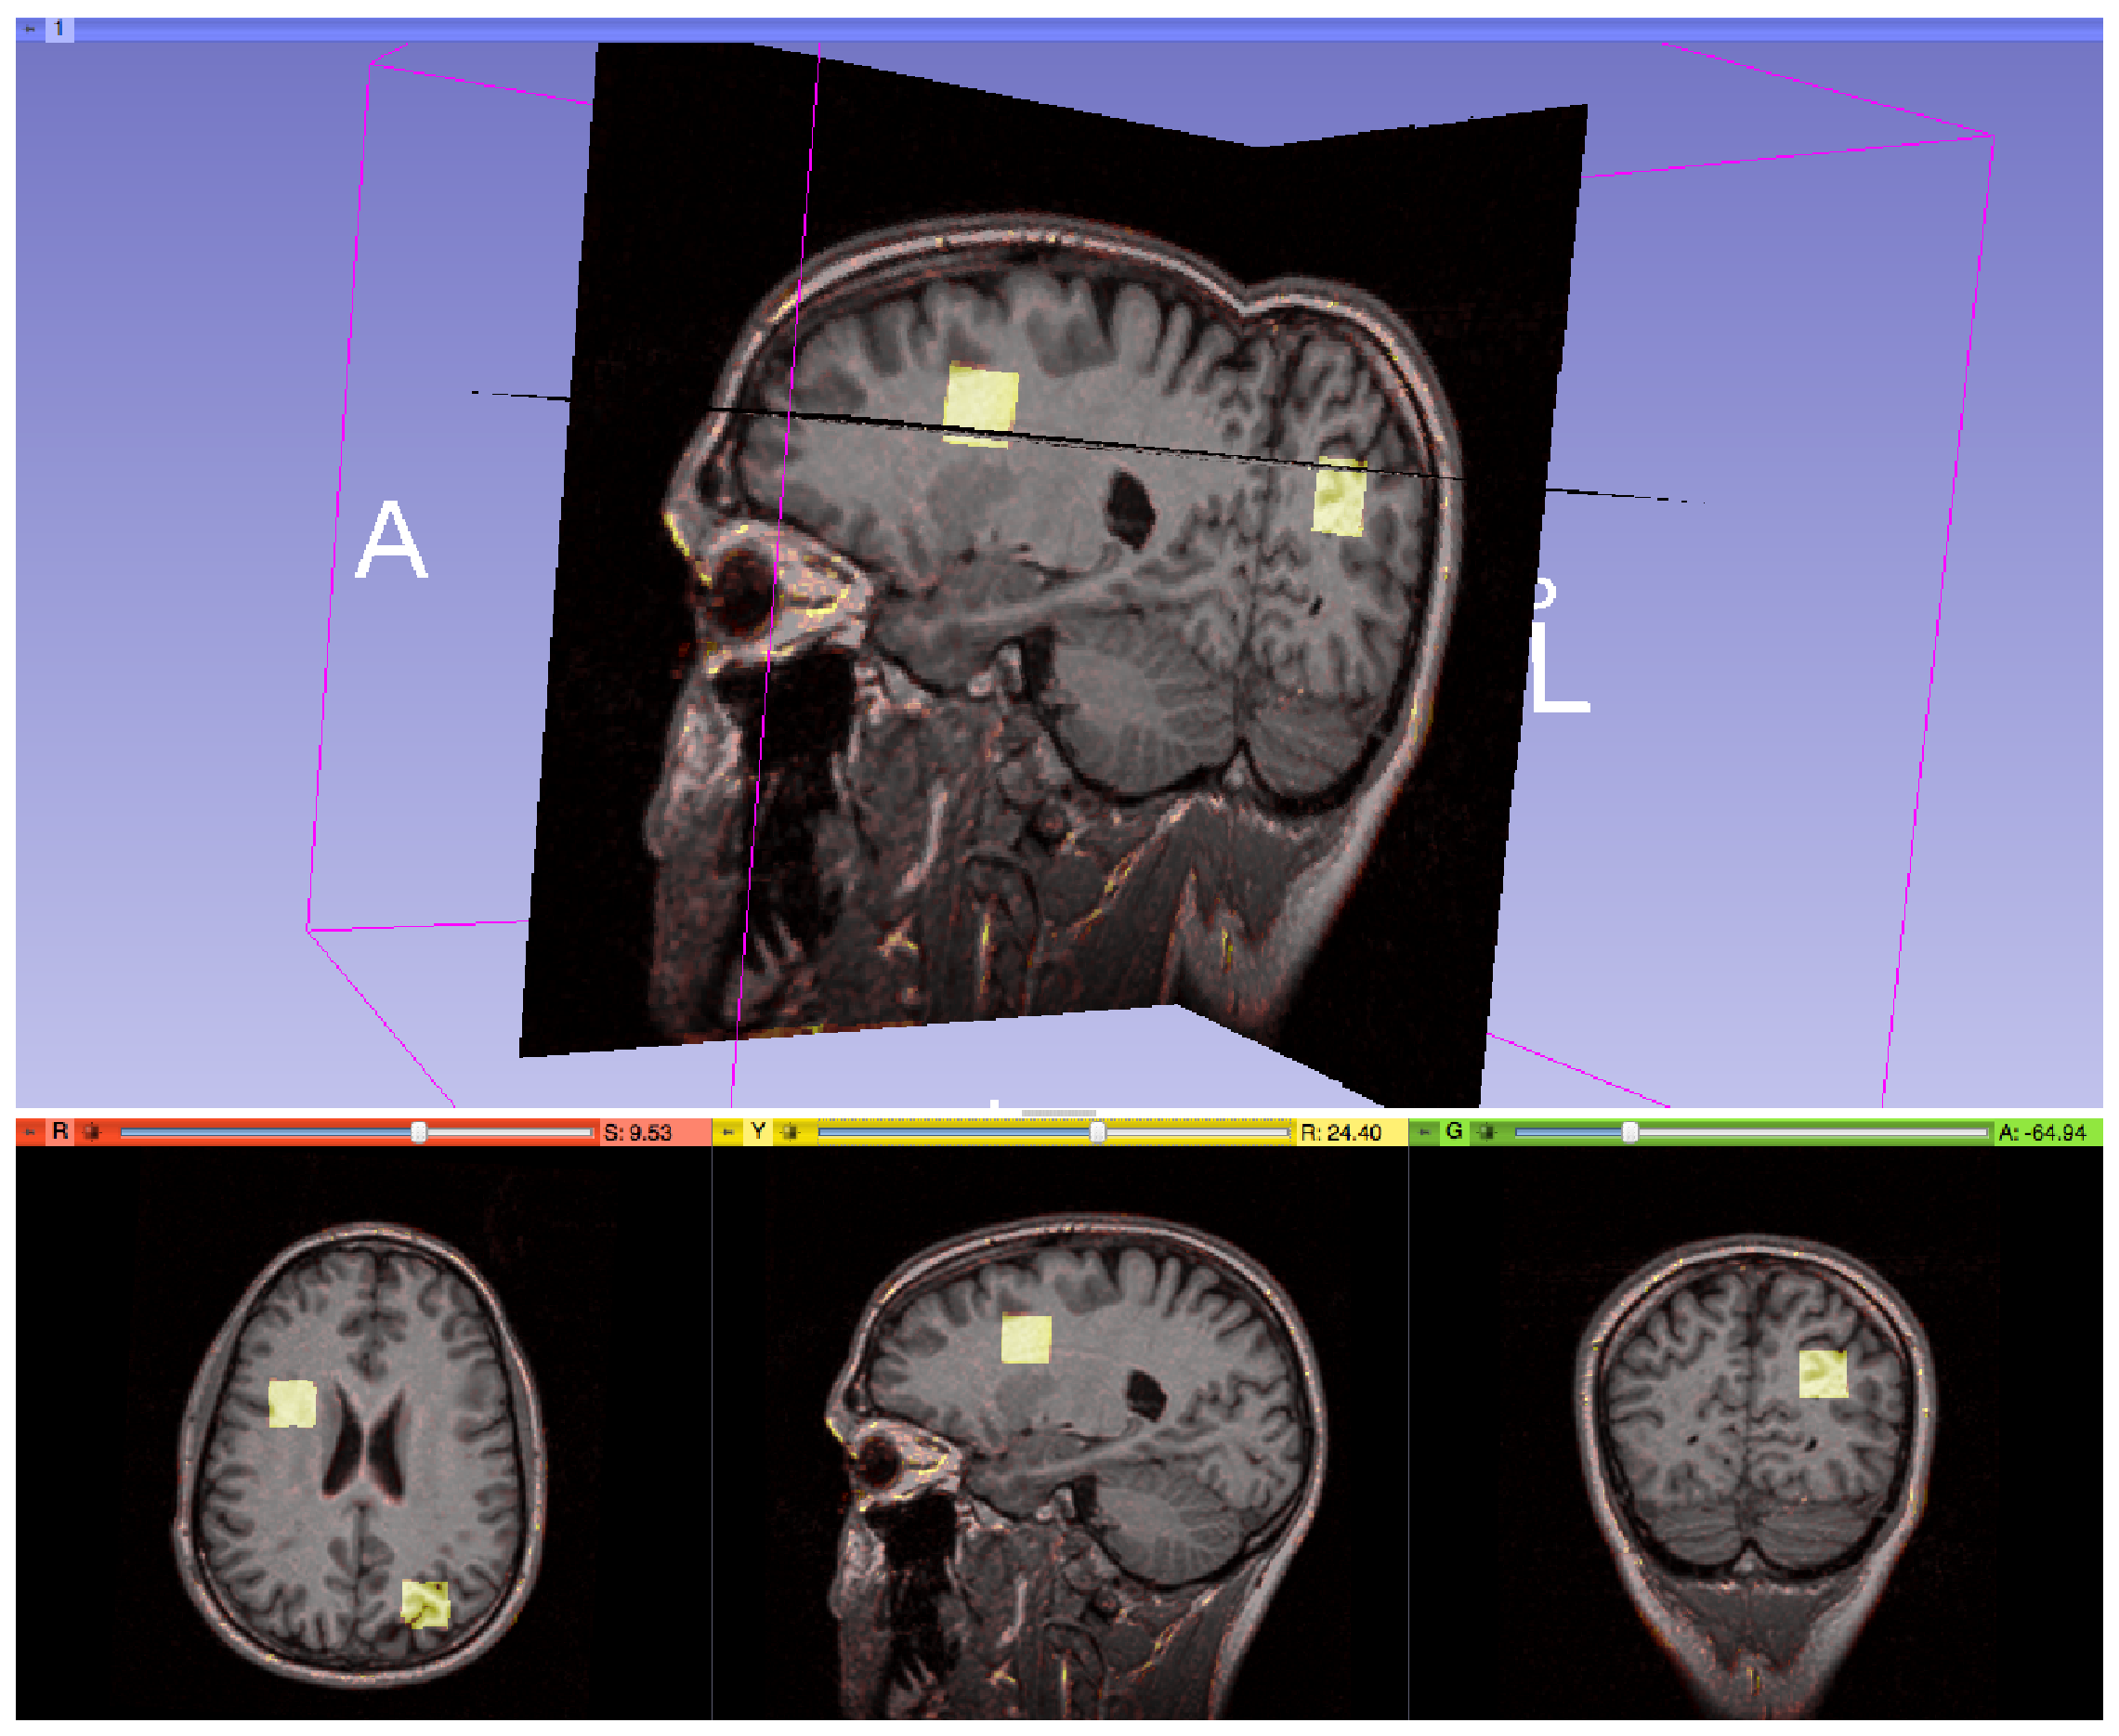
\includegraphics[scale=0.2]{/experiment_bigger/voxel_bigger2.eps}
  \caption{Artificial Large: Voxel-base method}
  \label{voxel_large2}
\end{figure}

\subsubsection{Tensor-based Method}
In the result obtained with this method the differences are easy to
find, but their borders are not properly defined. The method gives the
position of the differences but not their exact shape.

The parameters used to obtain this result are:
\begin{description}
\item \textit{Deformation field smoothing sigma:} 2.5
\item \textit{Shrinkage percentage:} 80
\item \textit{Growth percentage:} 65
\end{description}

\begin{figure}[H]
  \centering
  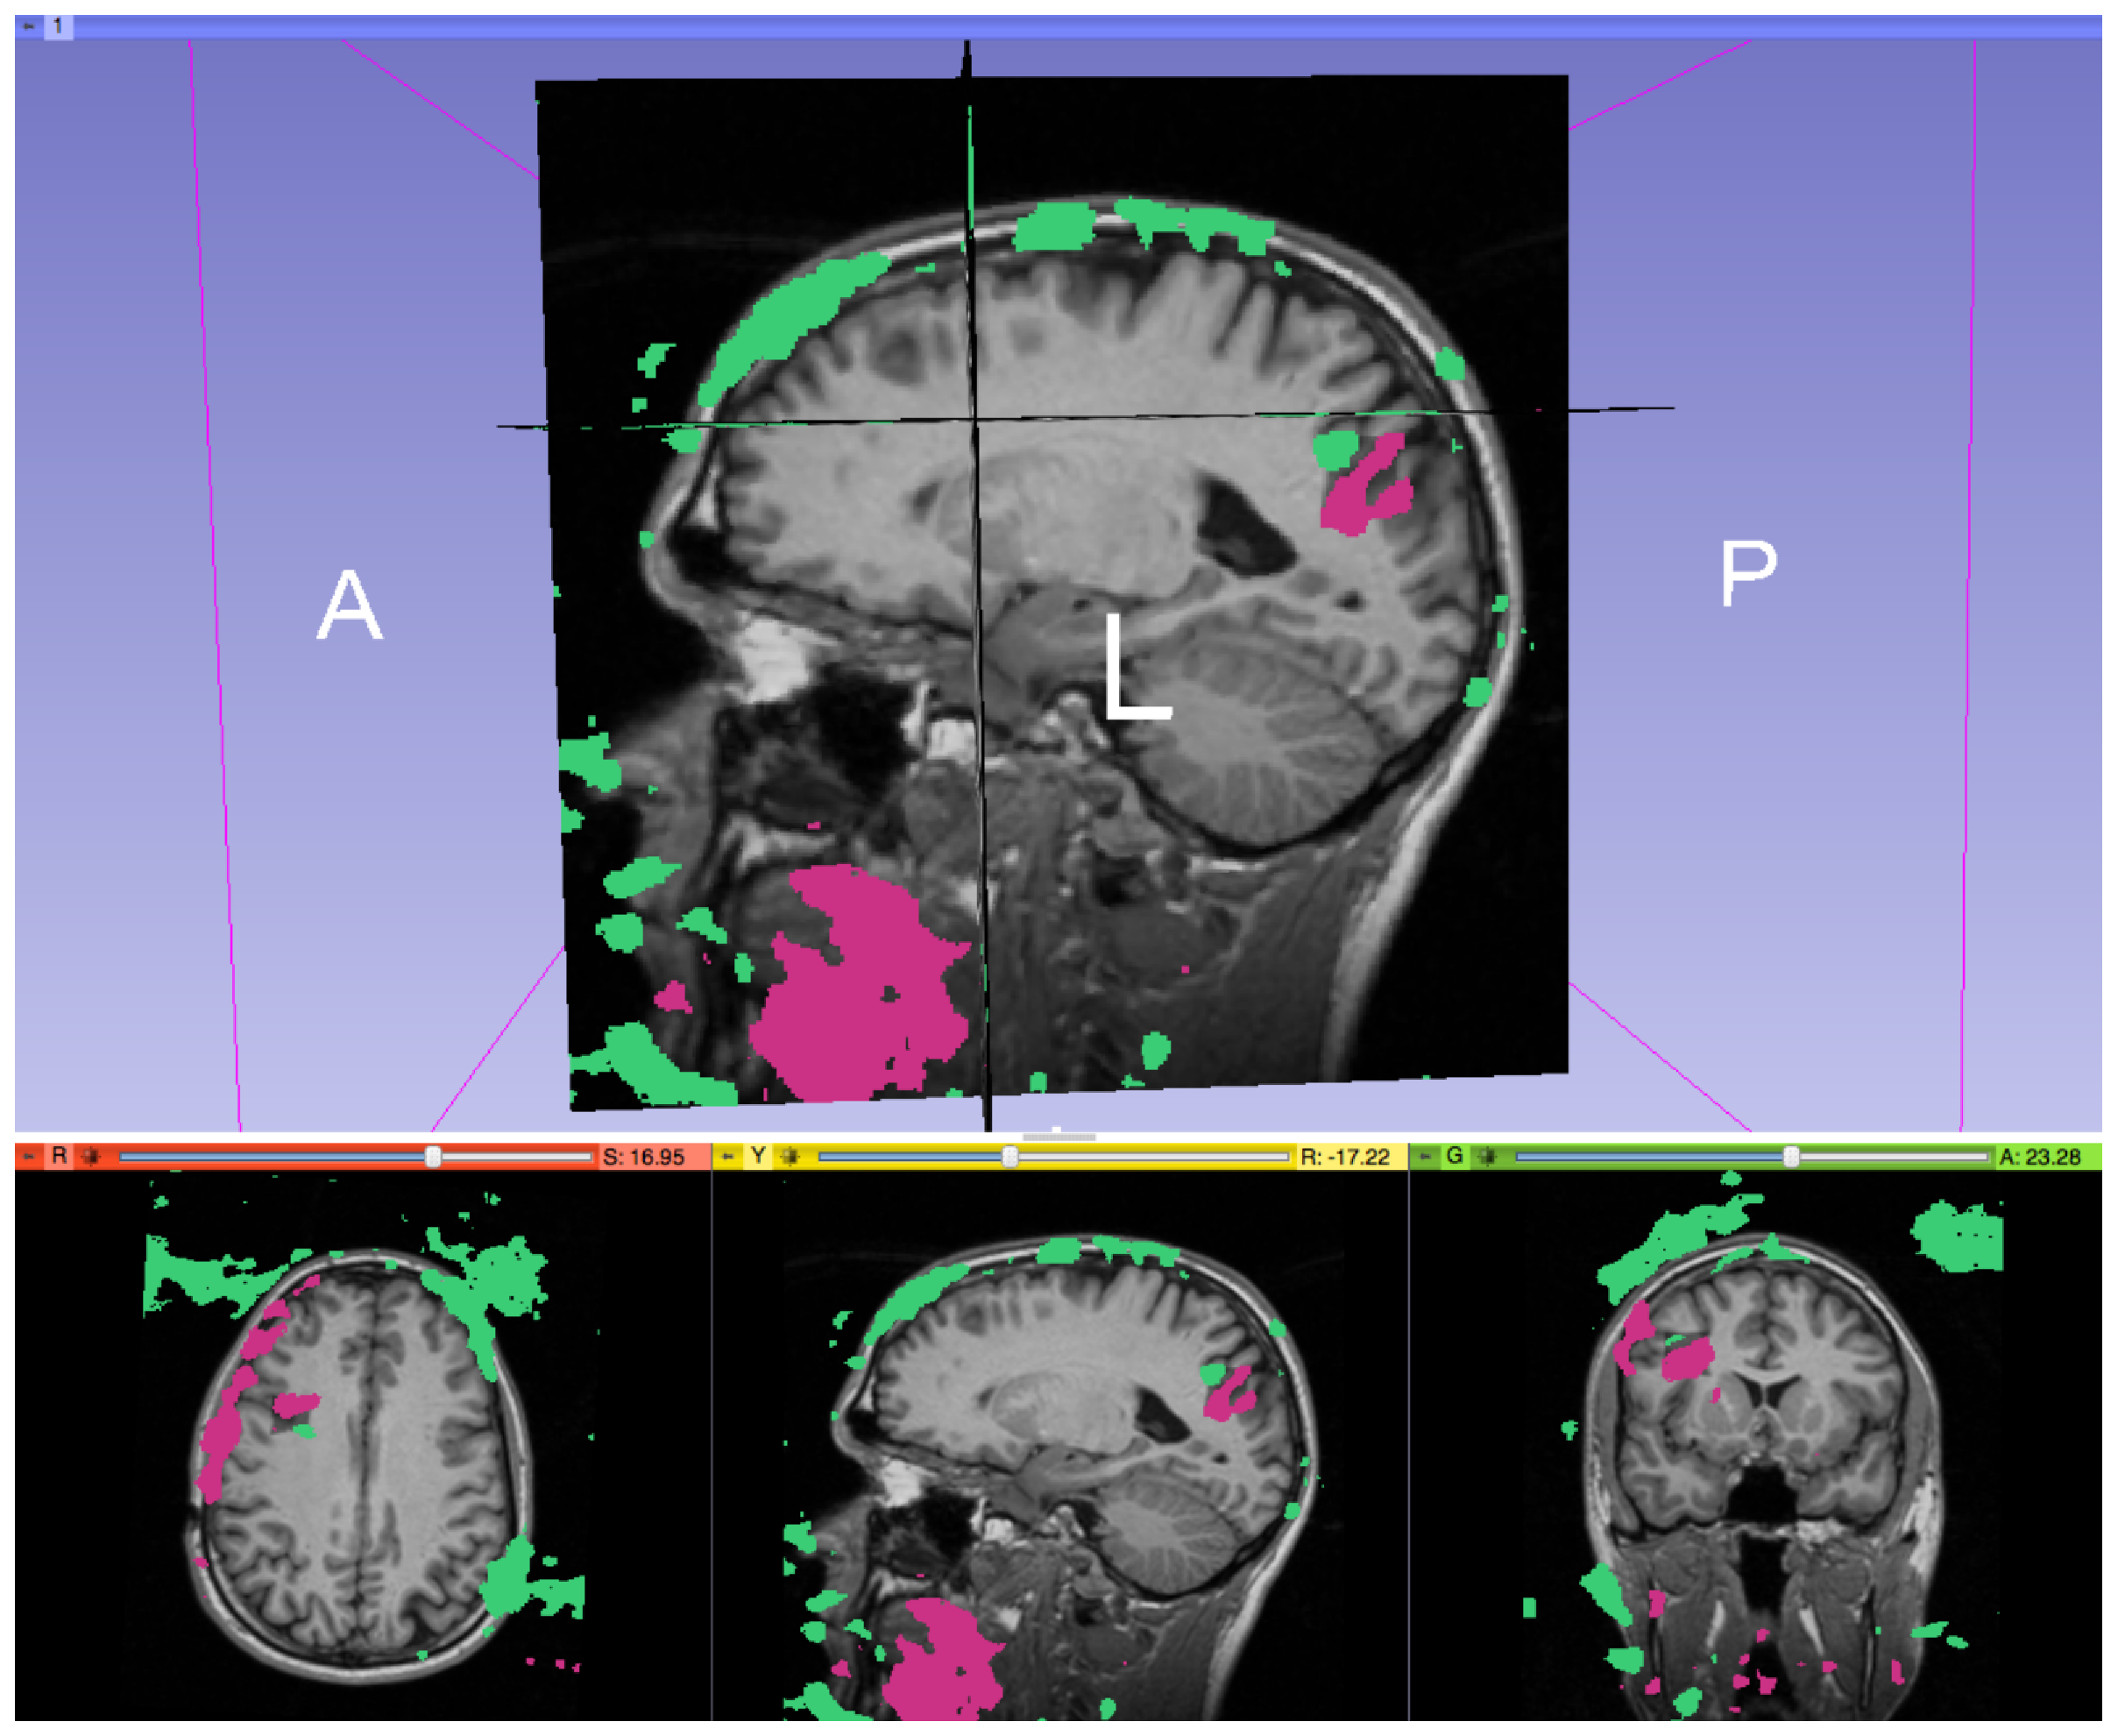
\includegraphics[scale=0.2]{/experiment_bigger/tensor80-65_bigger1.eps}
  \caption{Artificial Large: Tensor-base method}
  \label{voxel_large1}
\end{figure}

Another angle of the result:

\begin{figure}[H]
  \centering
  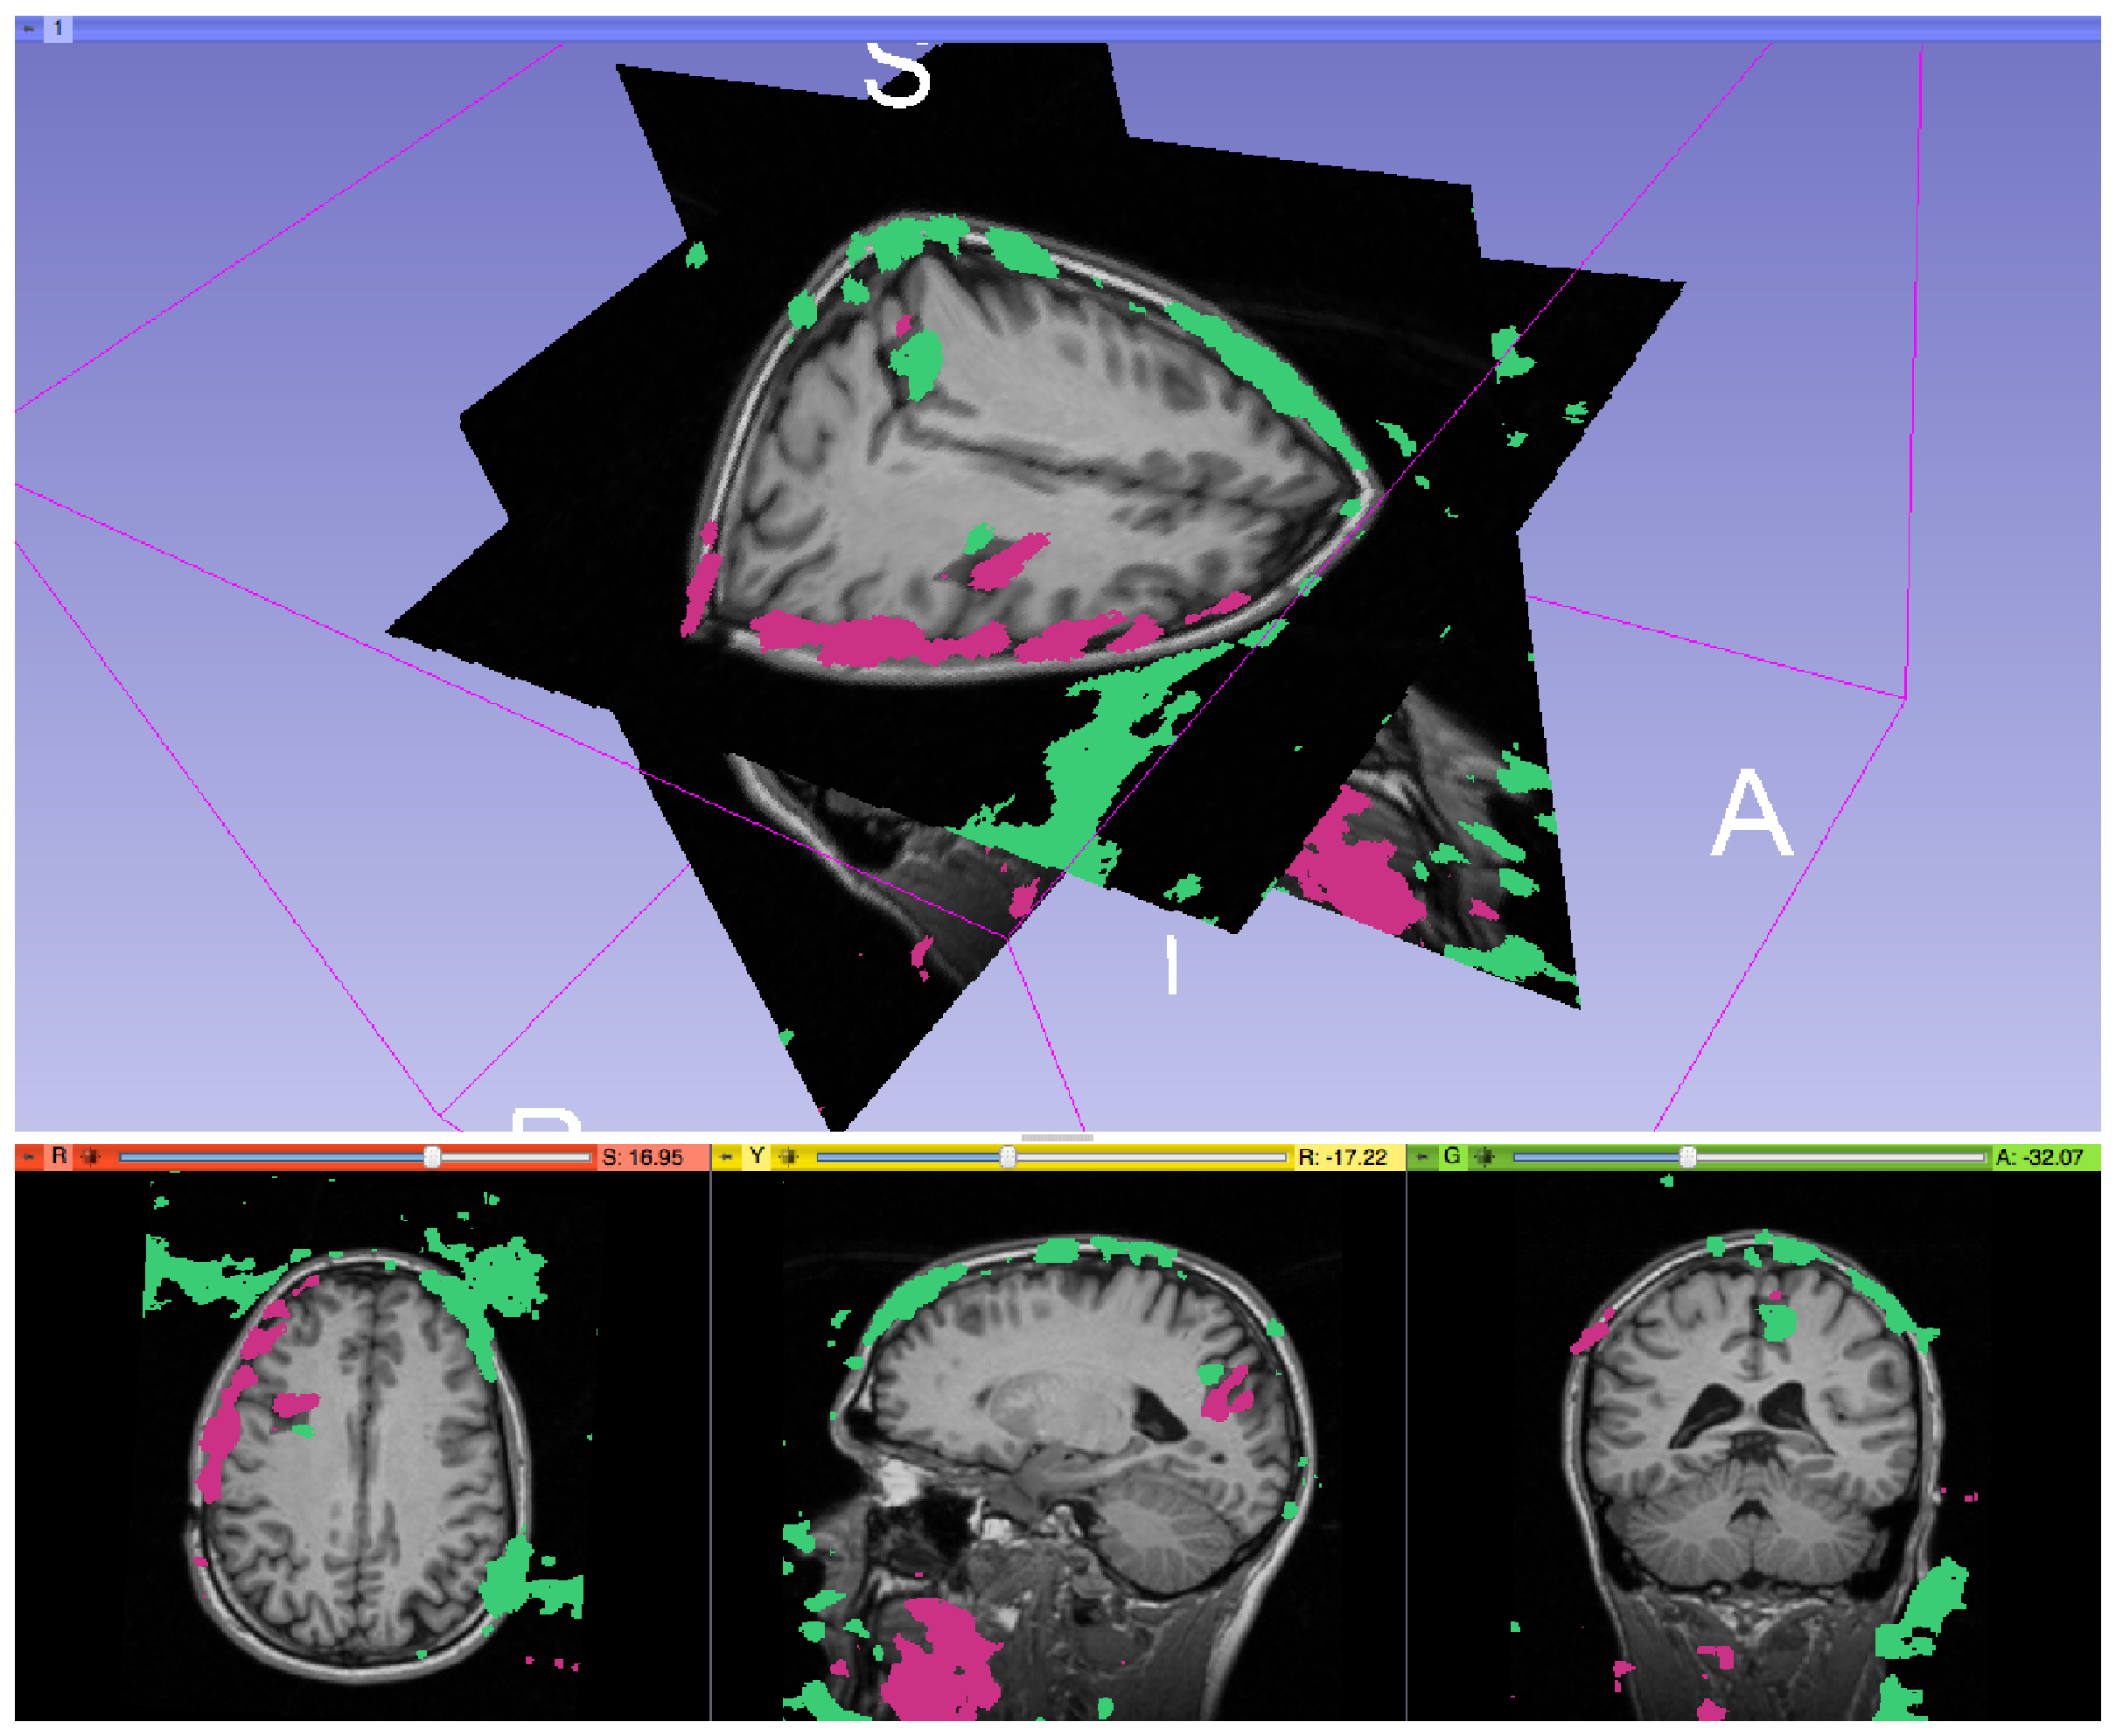
\includegraphics[scale=0.2]{/experiment_bigger/tensor80_65_bigger2.eps}
  \caption{Artificial Large: Tensor-base method}
  \label{voxel_large2}
\end{figure}


\subsection{Size: Medium}
\subsubsection{Voxel-based Method}

\subsubsection{Tensor-based Method}


\subsection{Size: Small}
\subsubsection{Voxel-based Method}




\subsubsection{Tensor-based Method}


\section{Real Differences Results}

\subsection{Patient 1}
This patient presents small differences in the parietal lobe, the
differences can be seen as red lines in the voxel-based method's result
and pink or green areas in the tensor-based method's result.

\subsubsection{Voxel-based Method}
The registration method used was \textit{Affine registration}.

\begin{figure}[H]
  \centering
  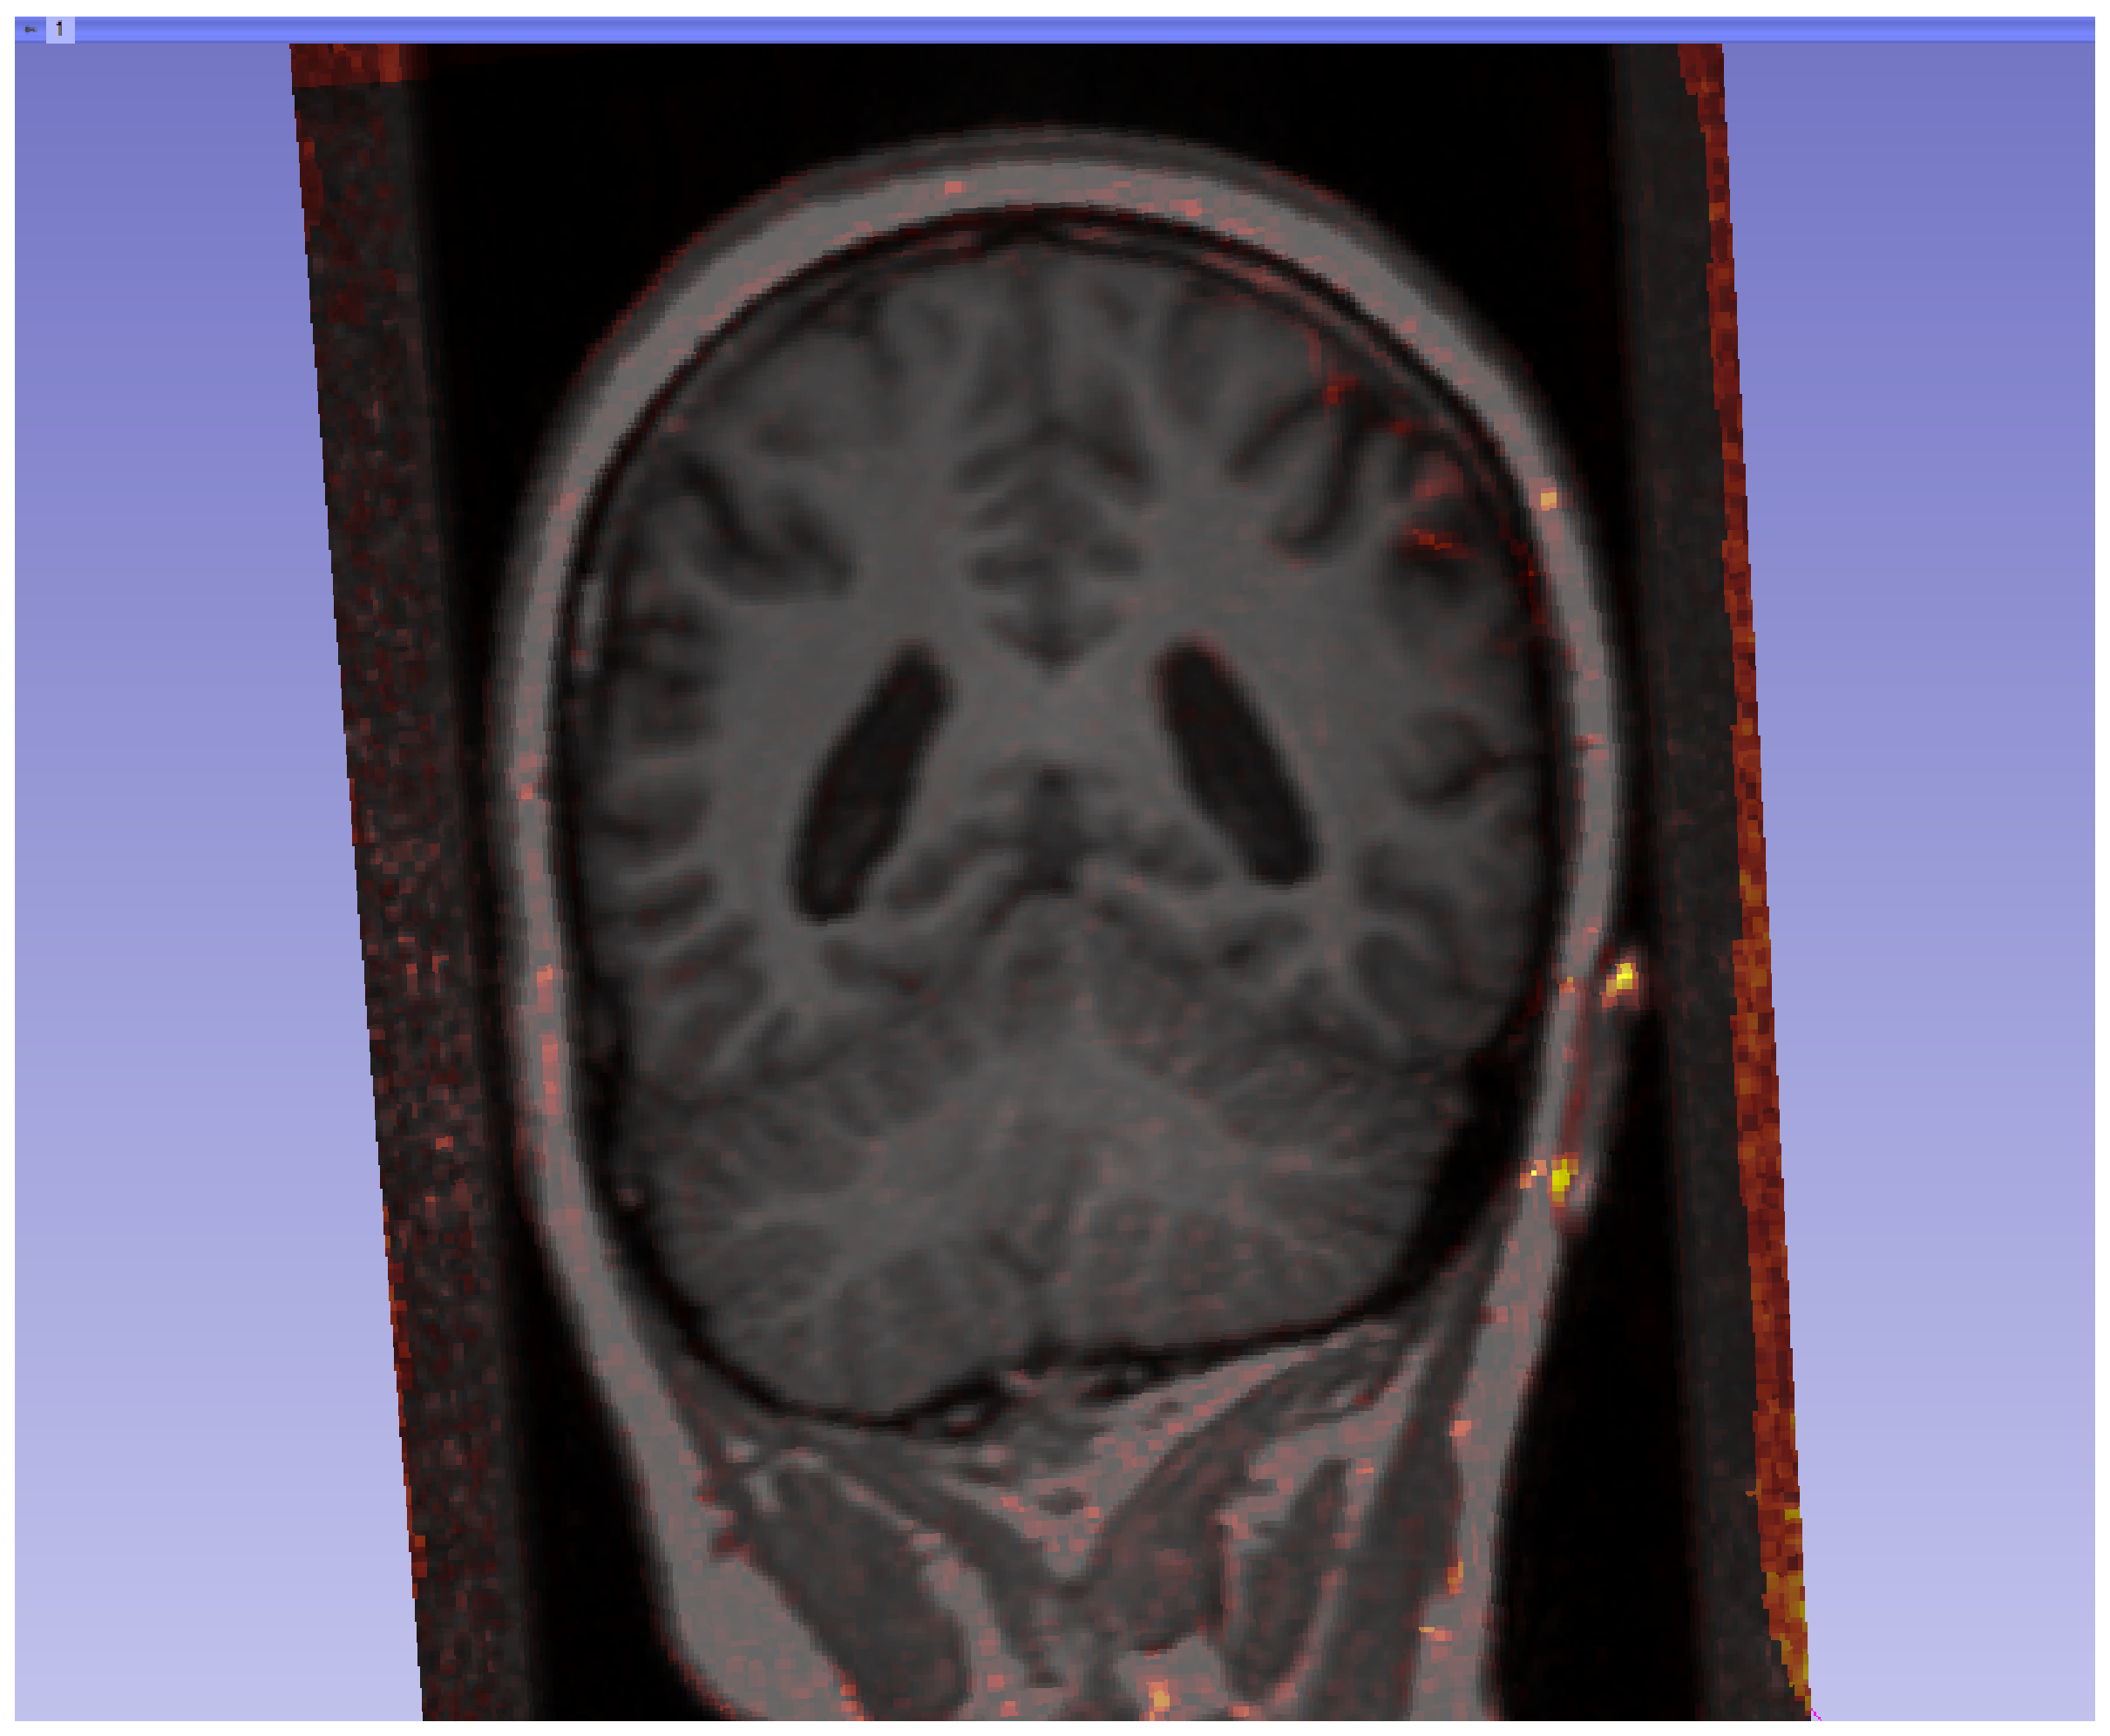
\includegraphics[scale=0.2]{/experiment_CL_P1/CL_Coronal.eps}
  \caption{Voxel-based method. Patient 1: Coronal plane}
  \label{CL_Coronal}
\end{figure}

\begin{figure}[H]
  \centering
  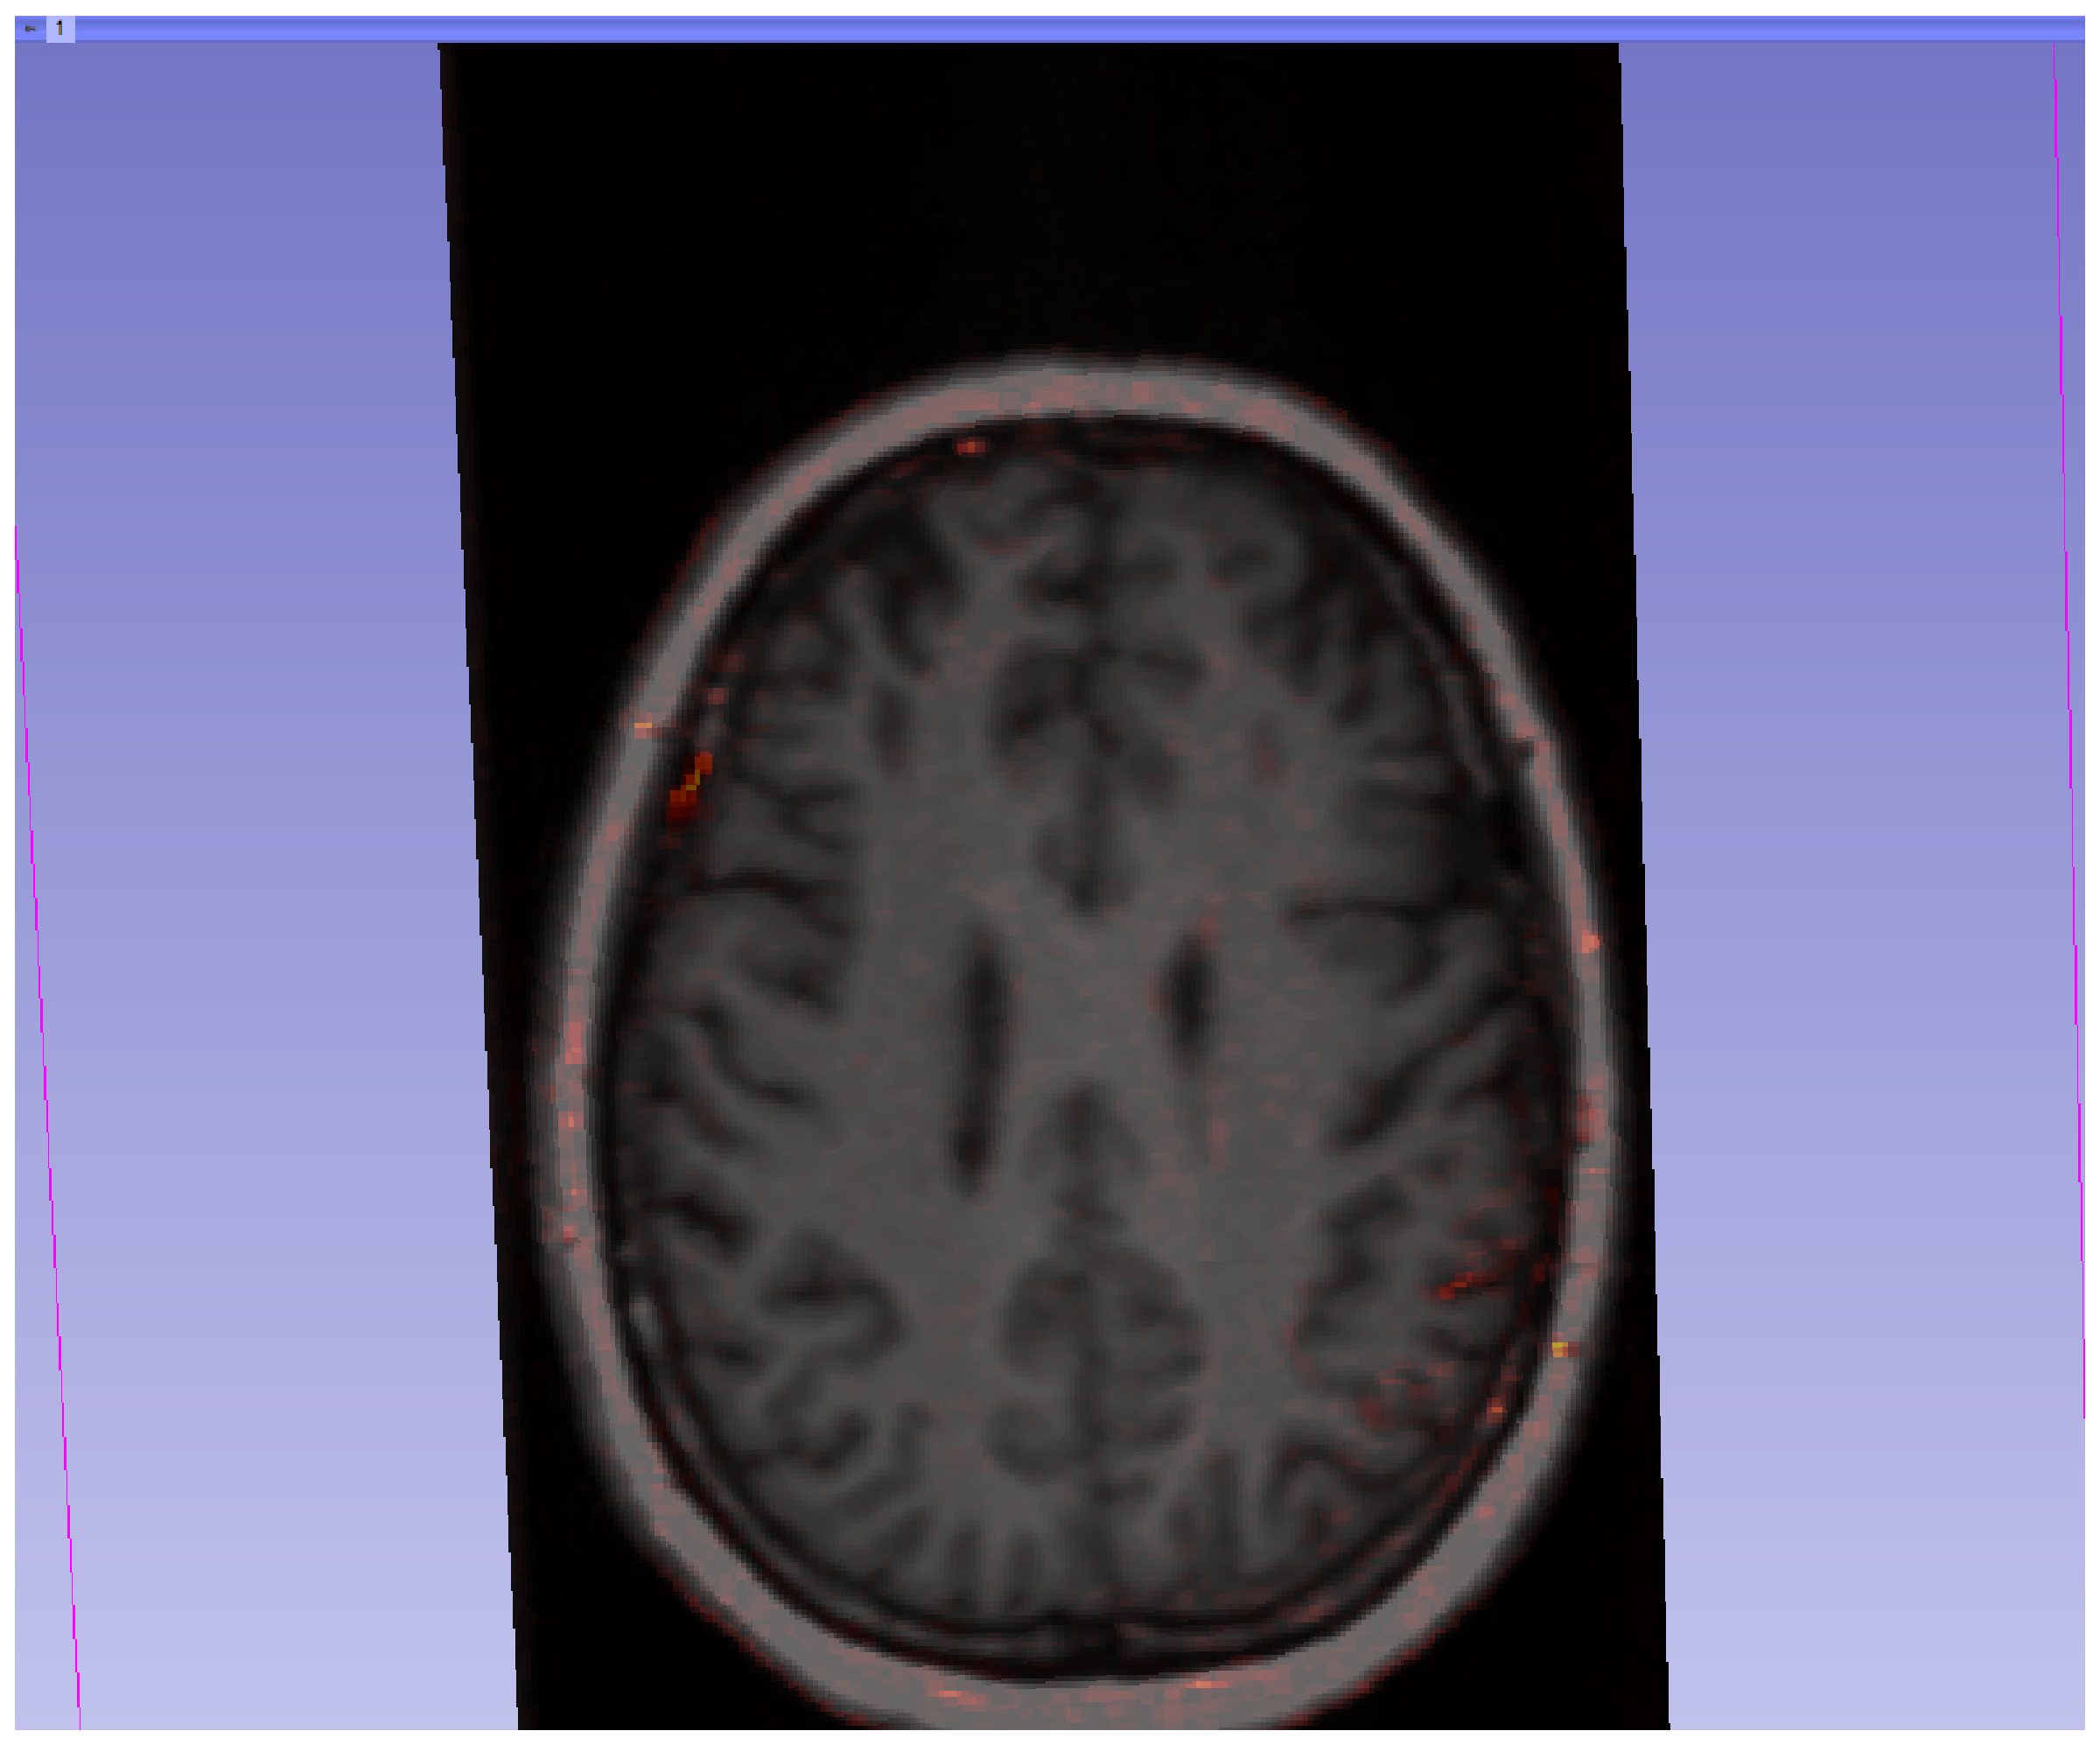
\includegraphics[scale=0.2]{/experiment_CL_P1/CL_Traversal.eps}
  \caption{Voxel-based method. Patient 1: Traversal plane}
  \label{CL_Traversal}
\end{figure}

\begin{figure}[H]
  \centering
  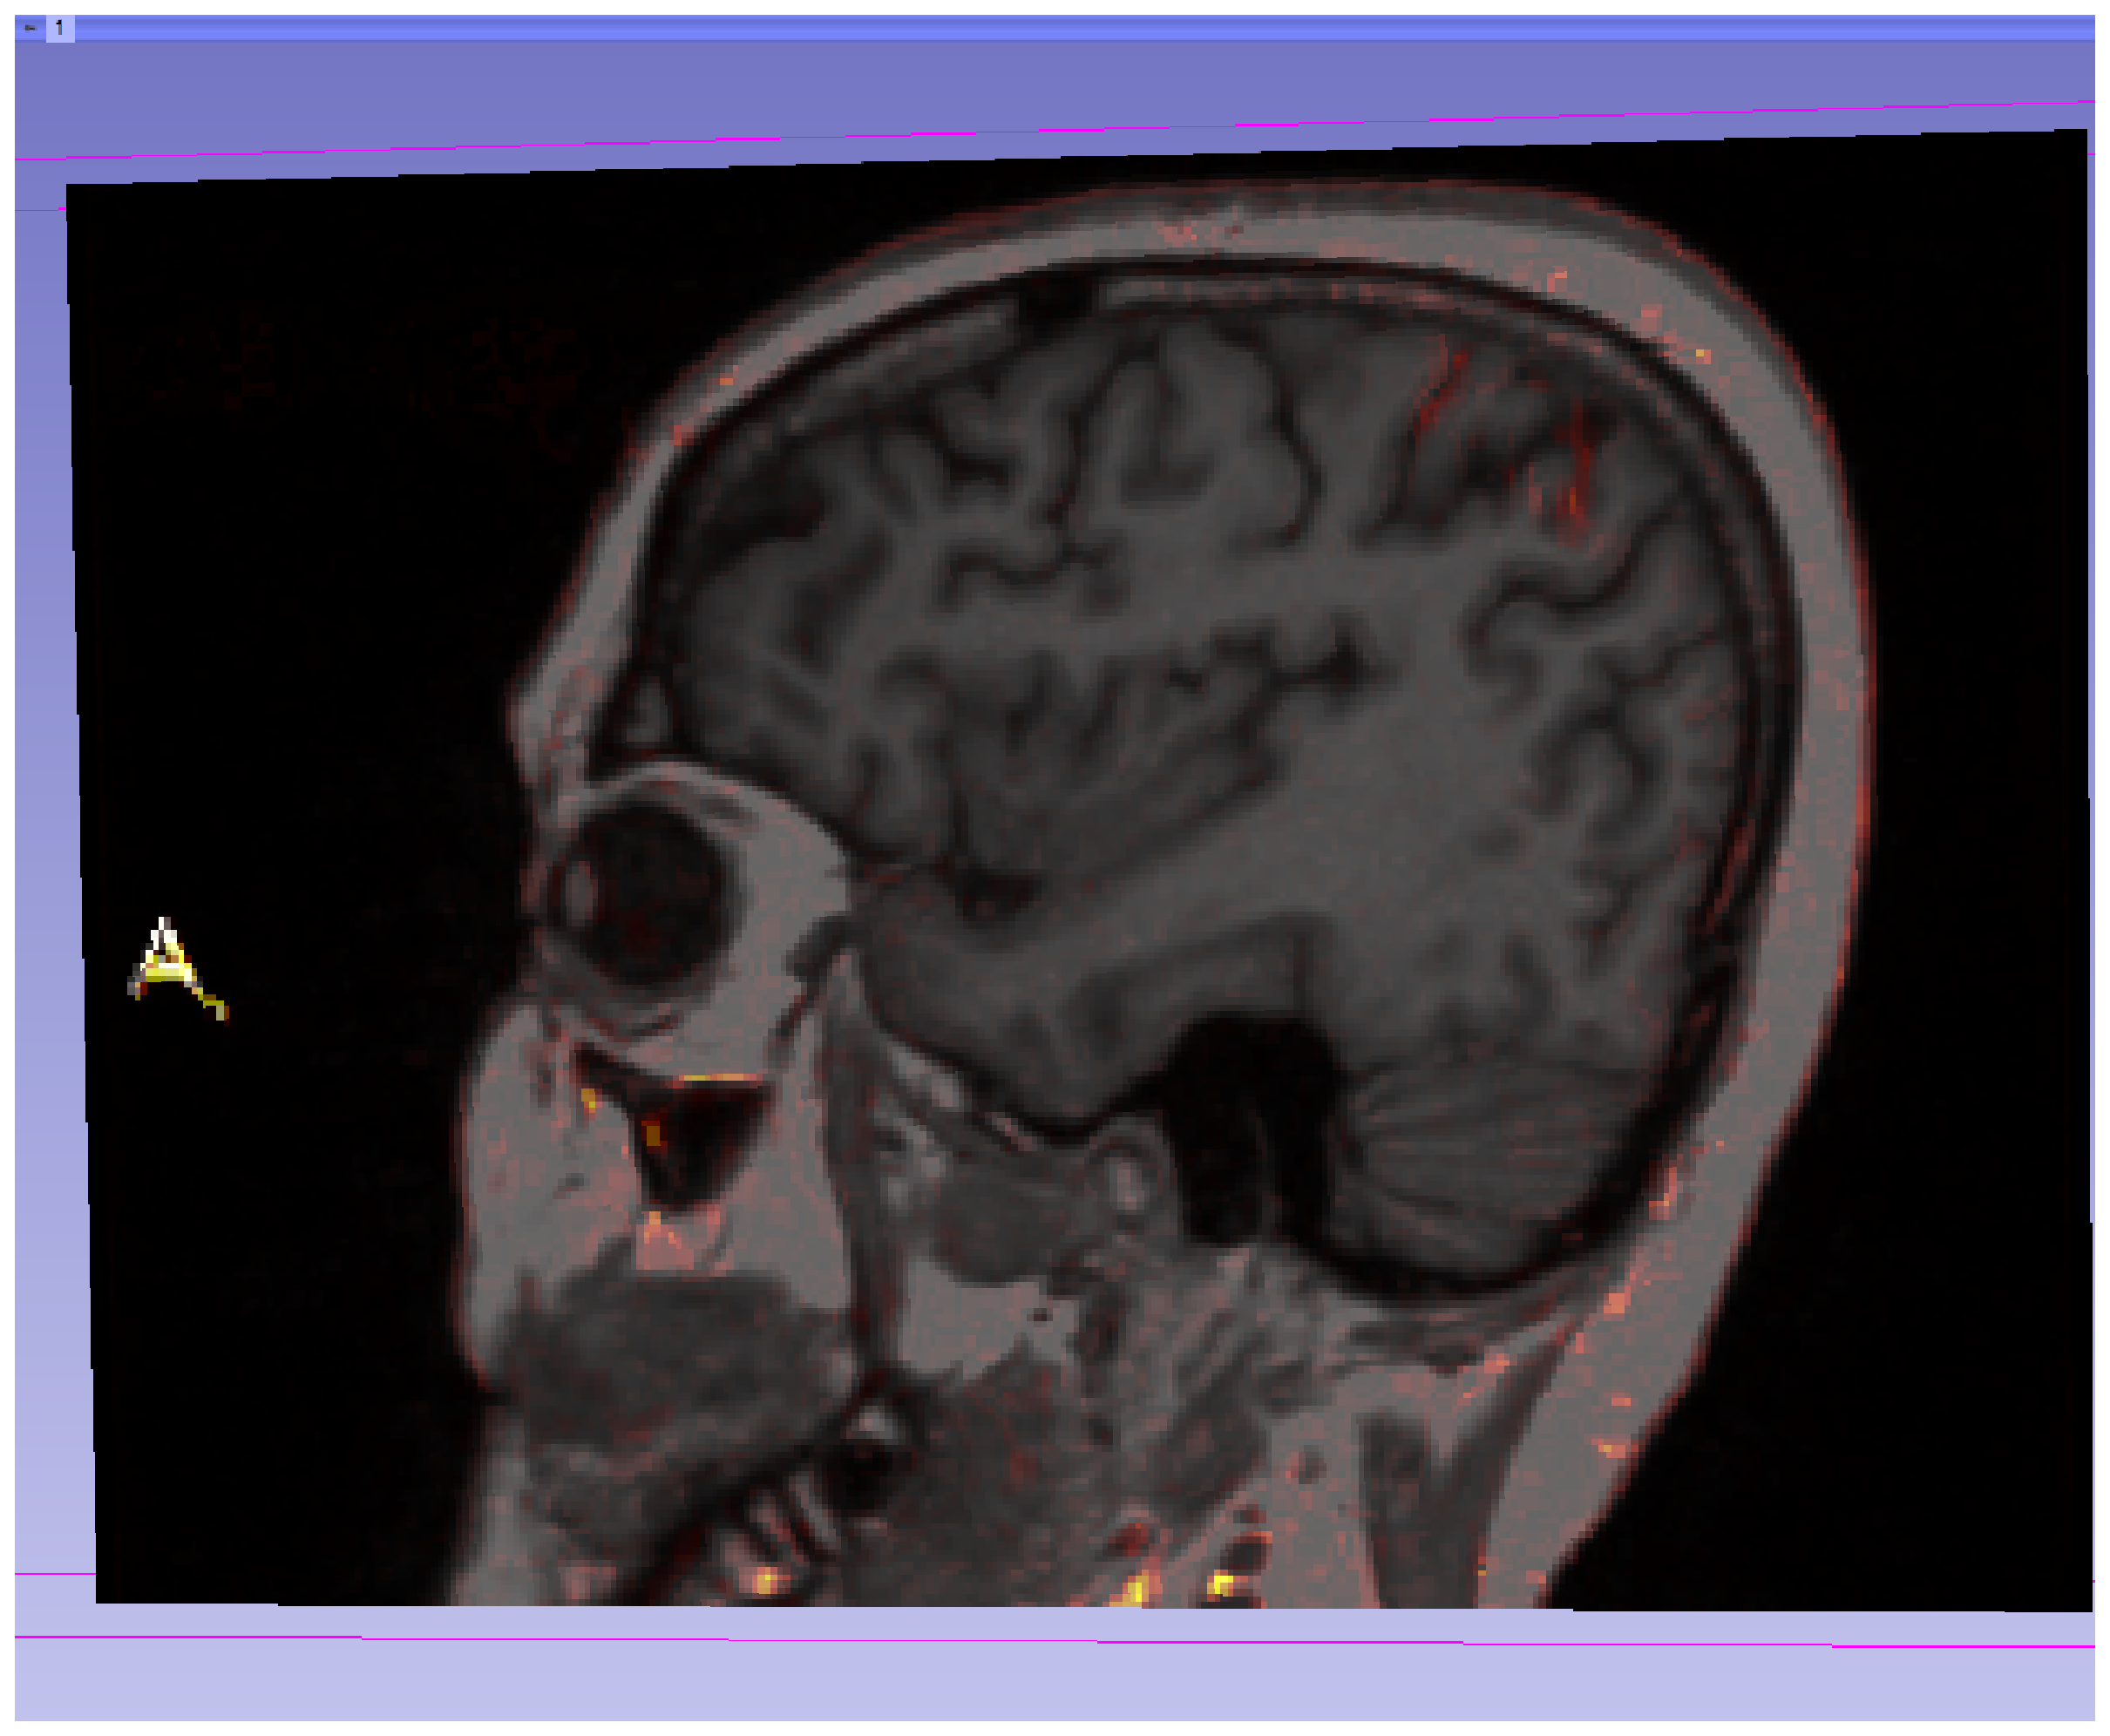
\includegraphics[scale=0.2]{/experiment_CL_P1/CL_Sagittal.eps}
  \caption{Voxel-based method. Patient 1: Sagittal plane}
  \label{CL_Sagittal}
\end{figure}


\subsubsection{Tensor-based Method}
Parameters used:
\begin{description}
\item \textit{Deformation field smoothing sigma:} 2.5
\item \textit{Shrinkage percentage:} 70
\item \textit{Growth percentage:} 75
\end{description}

\begin{figure}[H]
  \centering
  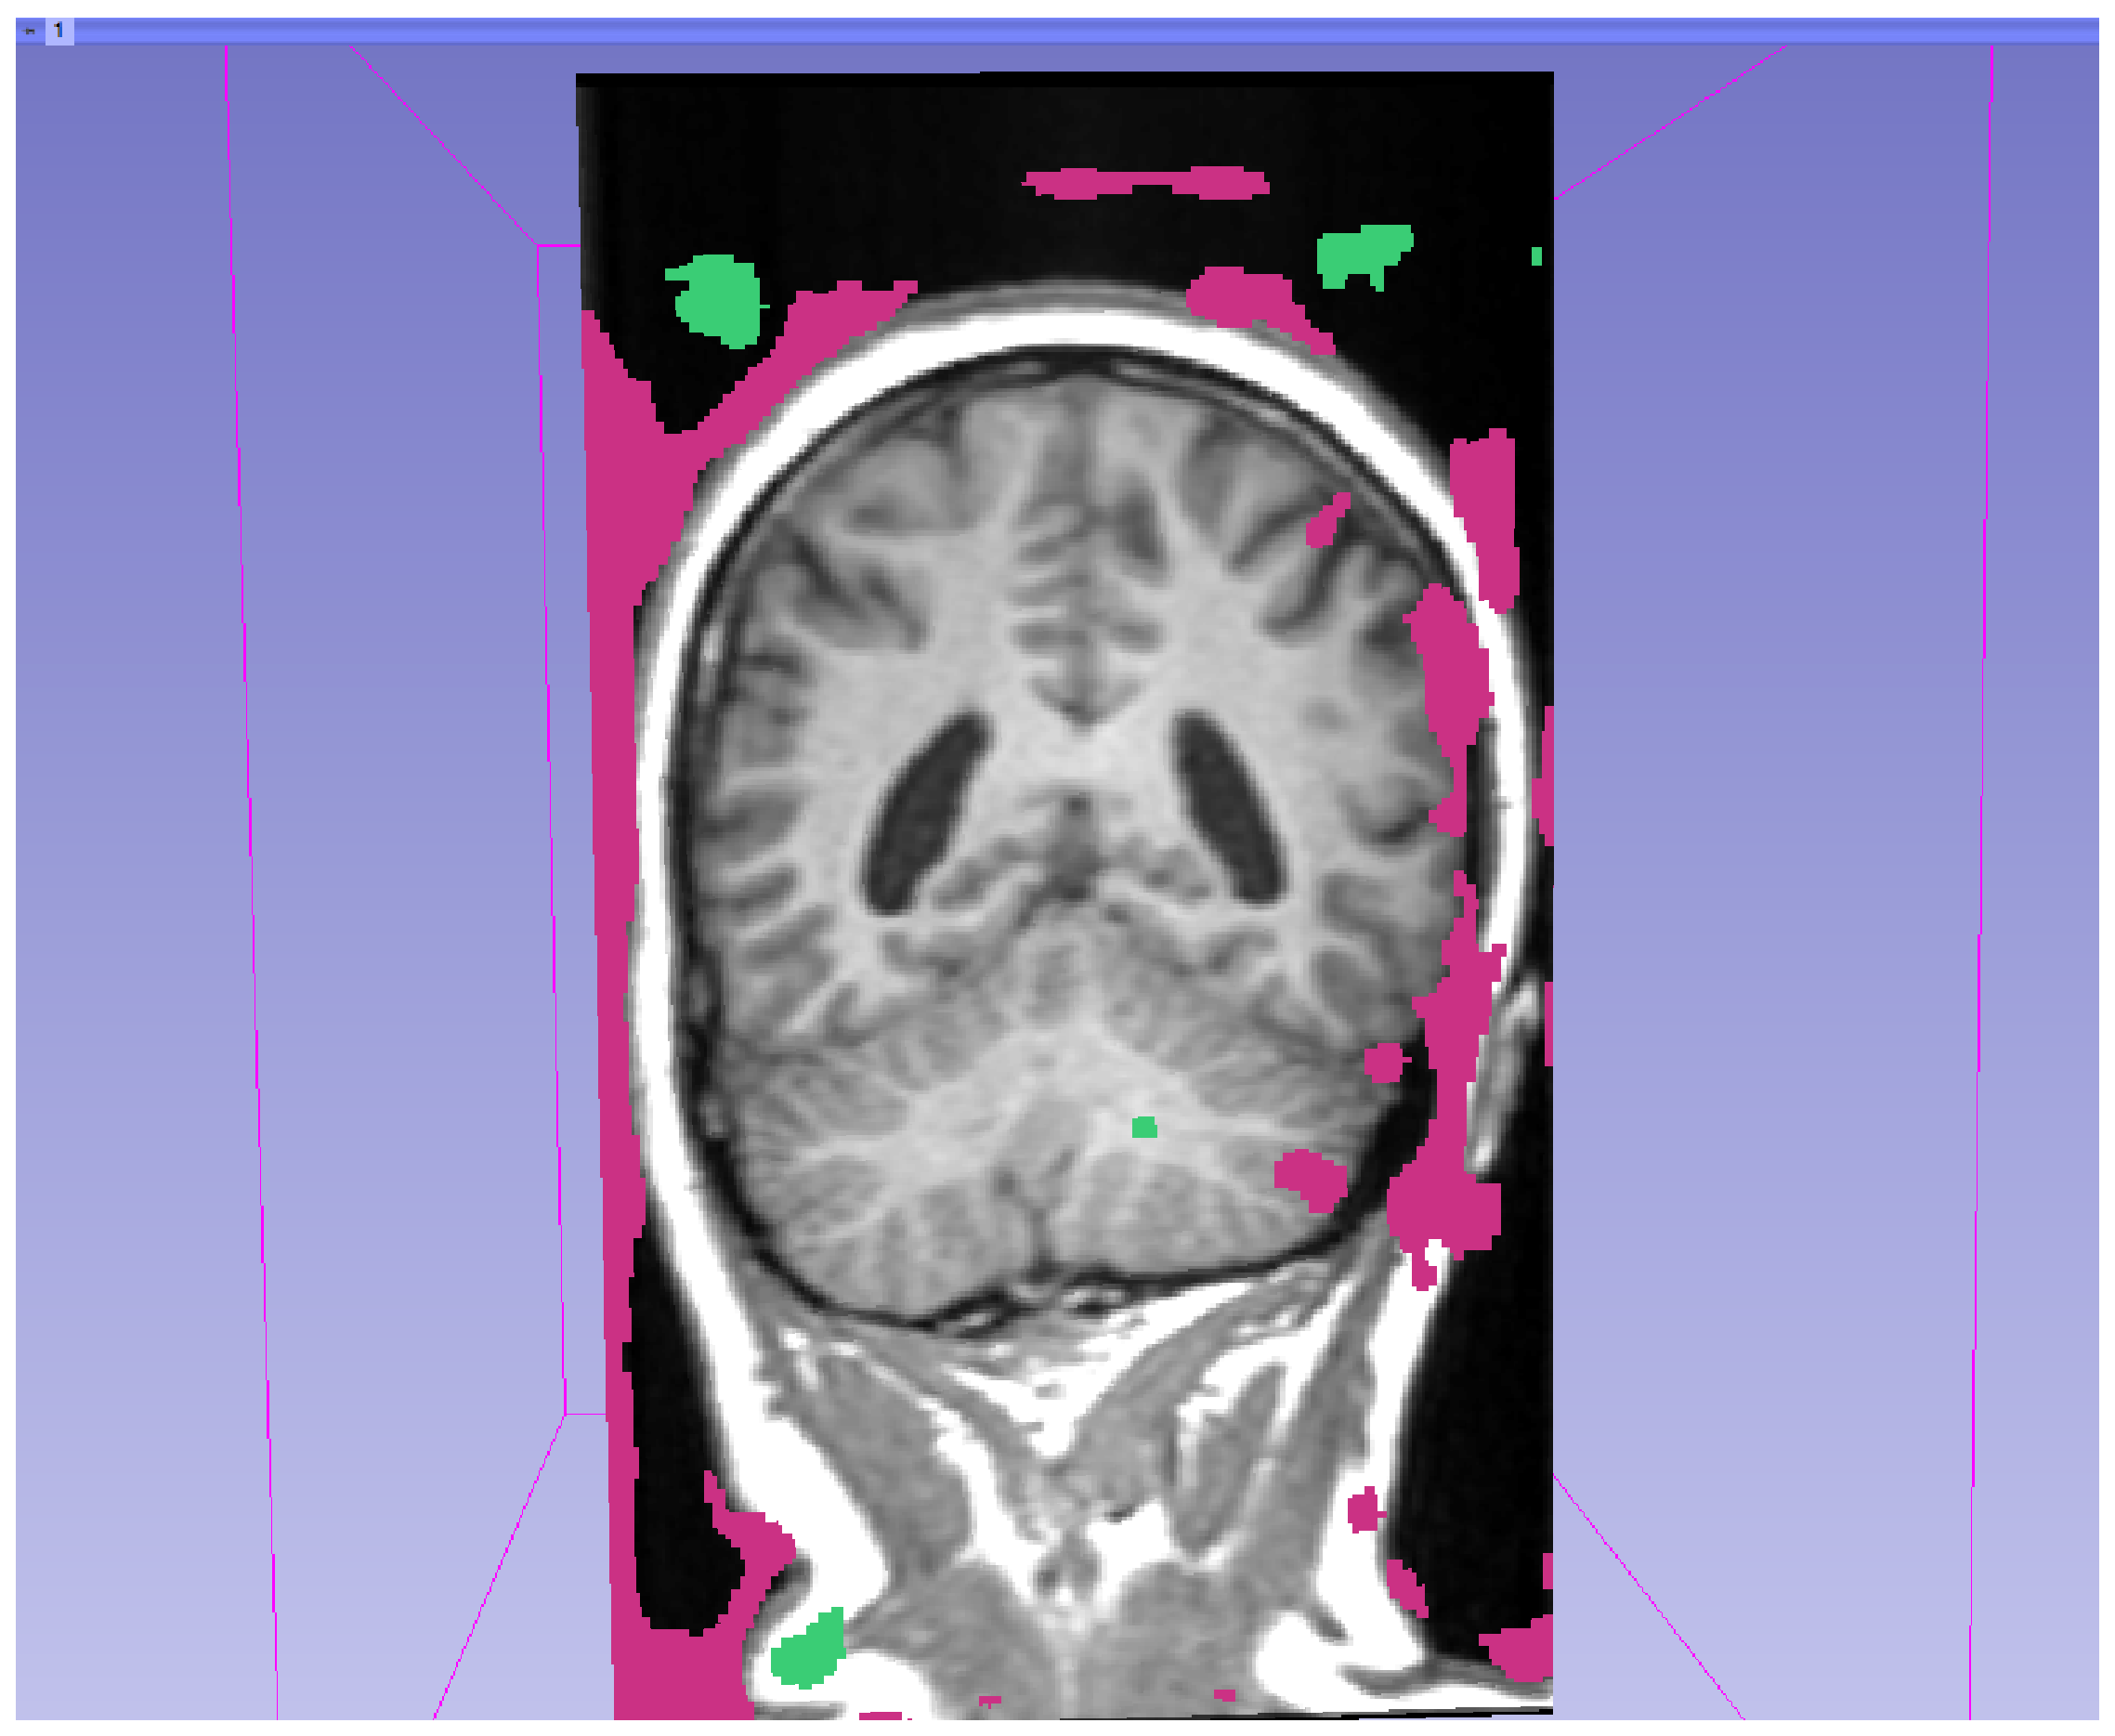
\includegraphics[scale=0.2]{/experiment_CL_P1/CL_Tensor_Coronal.eps}
  \caption{Tensor-based method. Patient 1: Coronal plane}
  \label{CL_TCoronal}
\end{figure}

\begin{figure}[H]
  \centering
  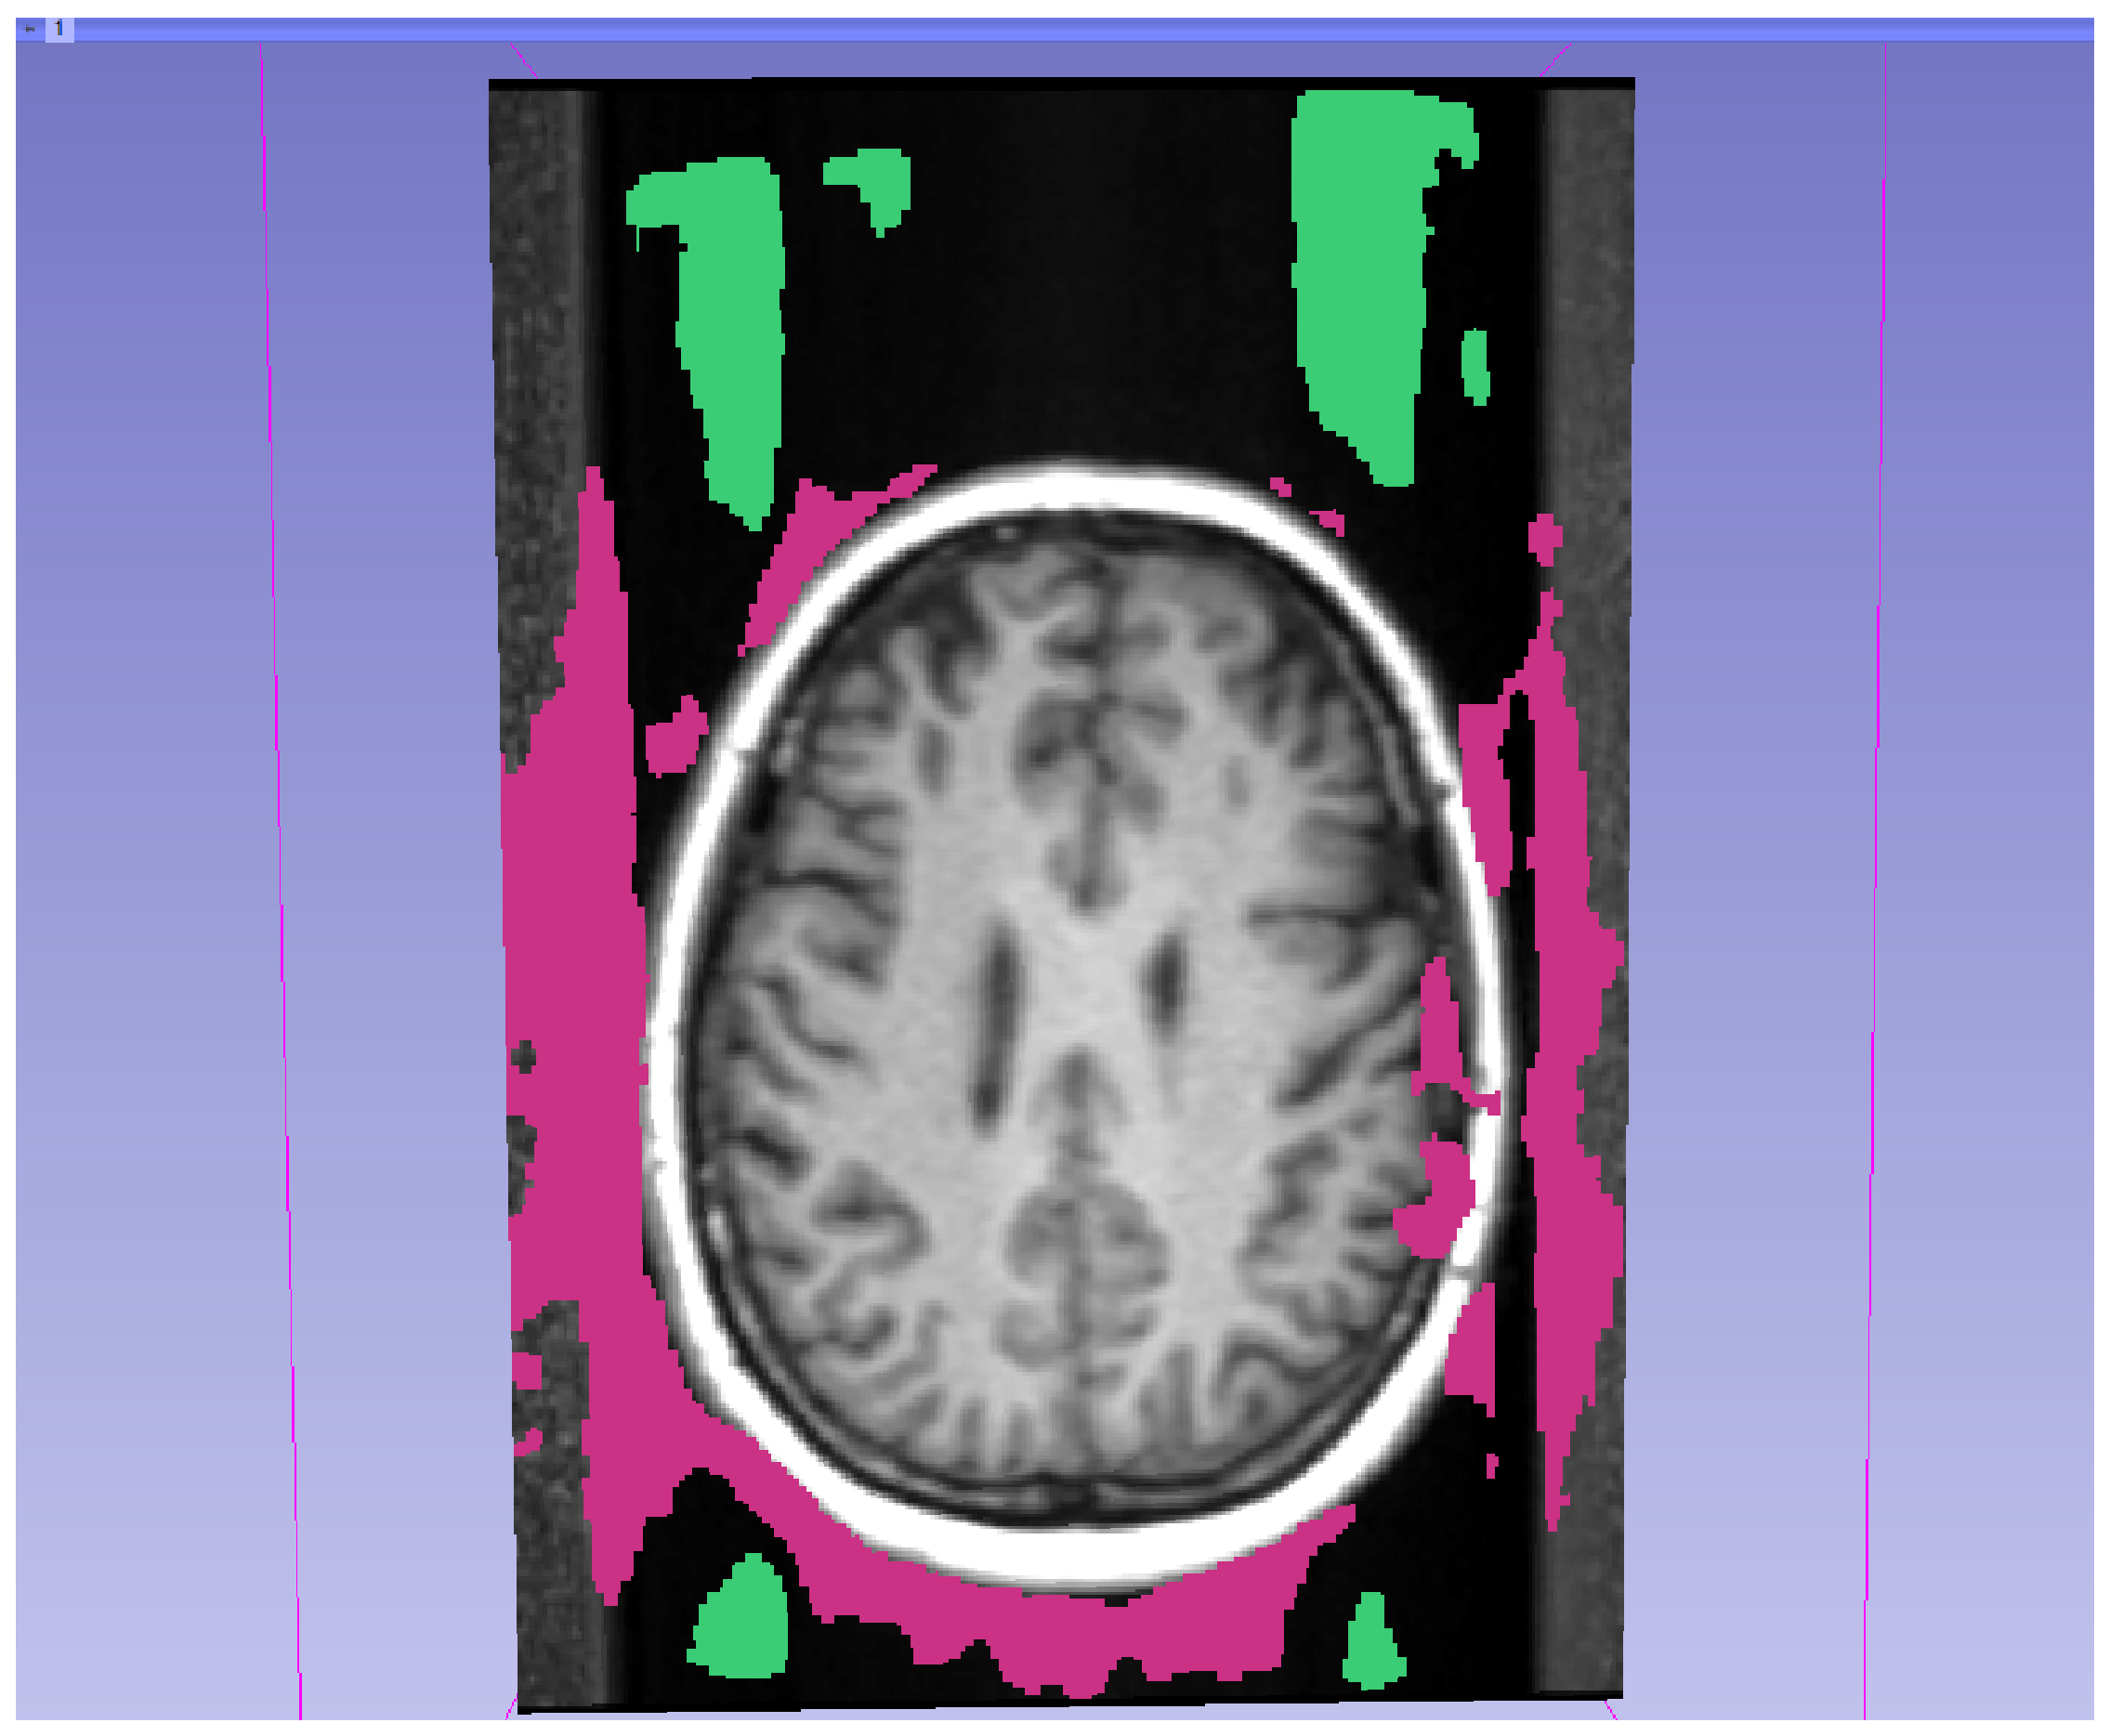
\includegraphics[scale=0.2]{/experiment_CL_P1/CL_Tensor_Traversal.eps}
  \caption{Tensor-based method. Patient 1: Traversal plane}
  \label{CL_TTraversal}
\end{figure}

\begin{figure}[H]
  \centering
  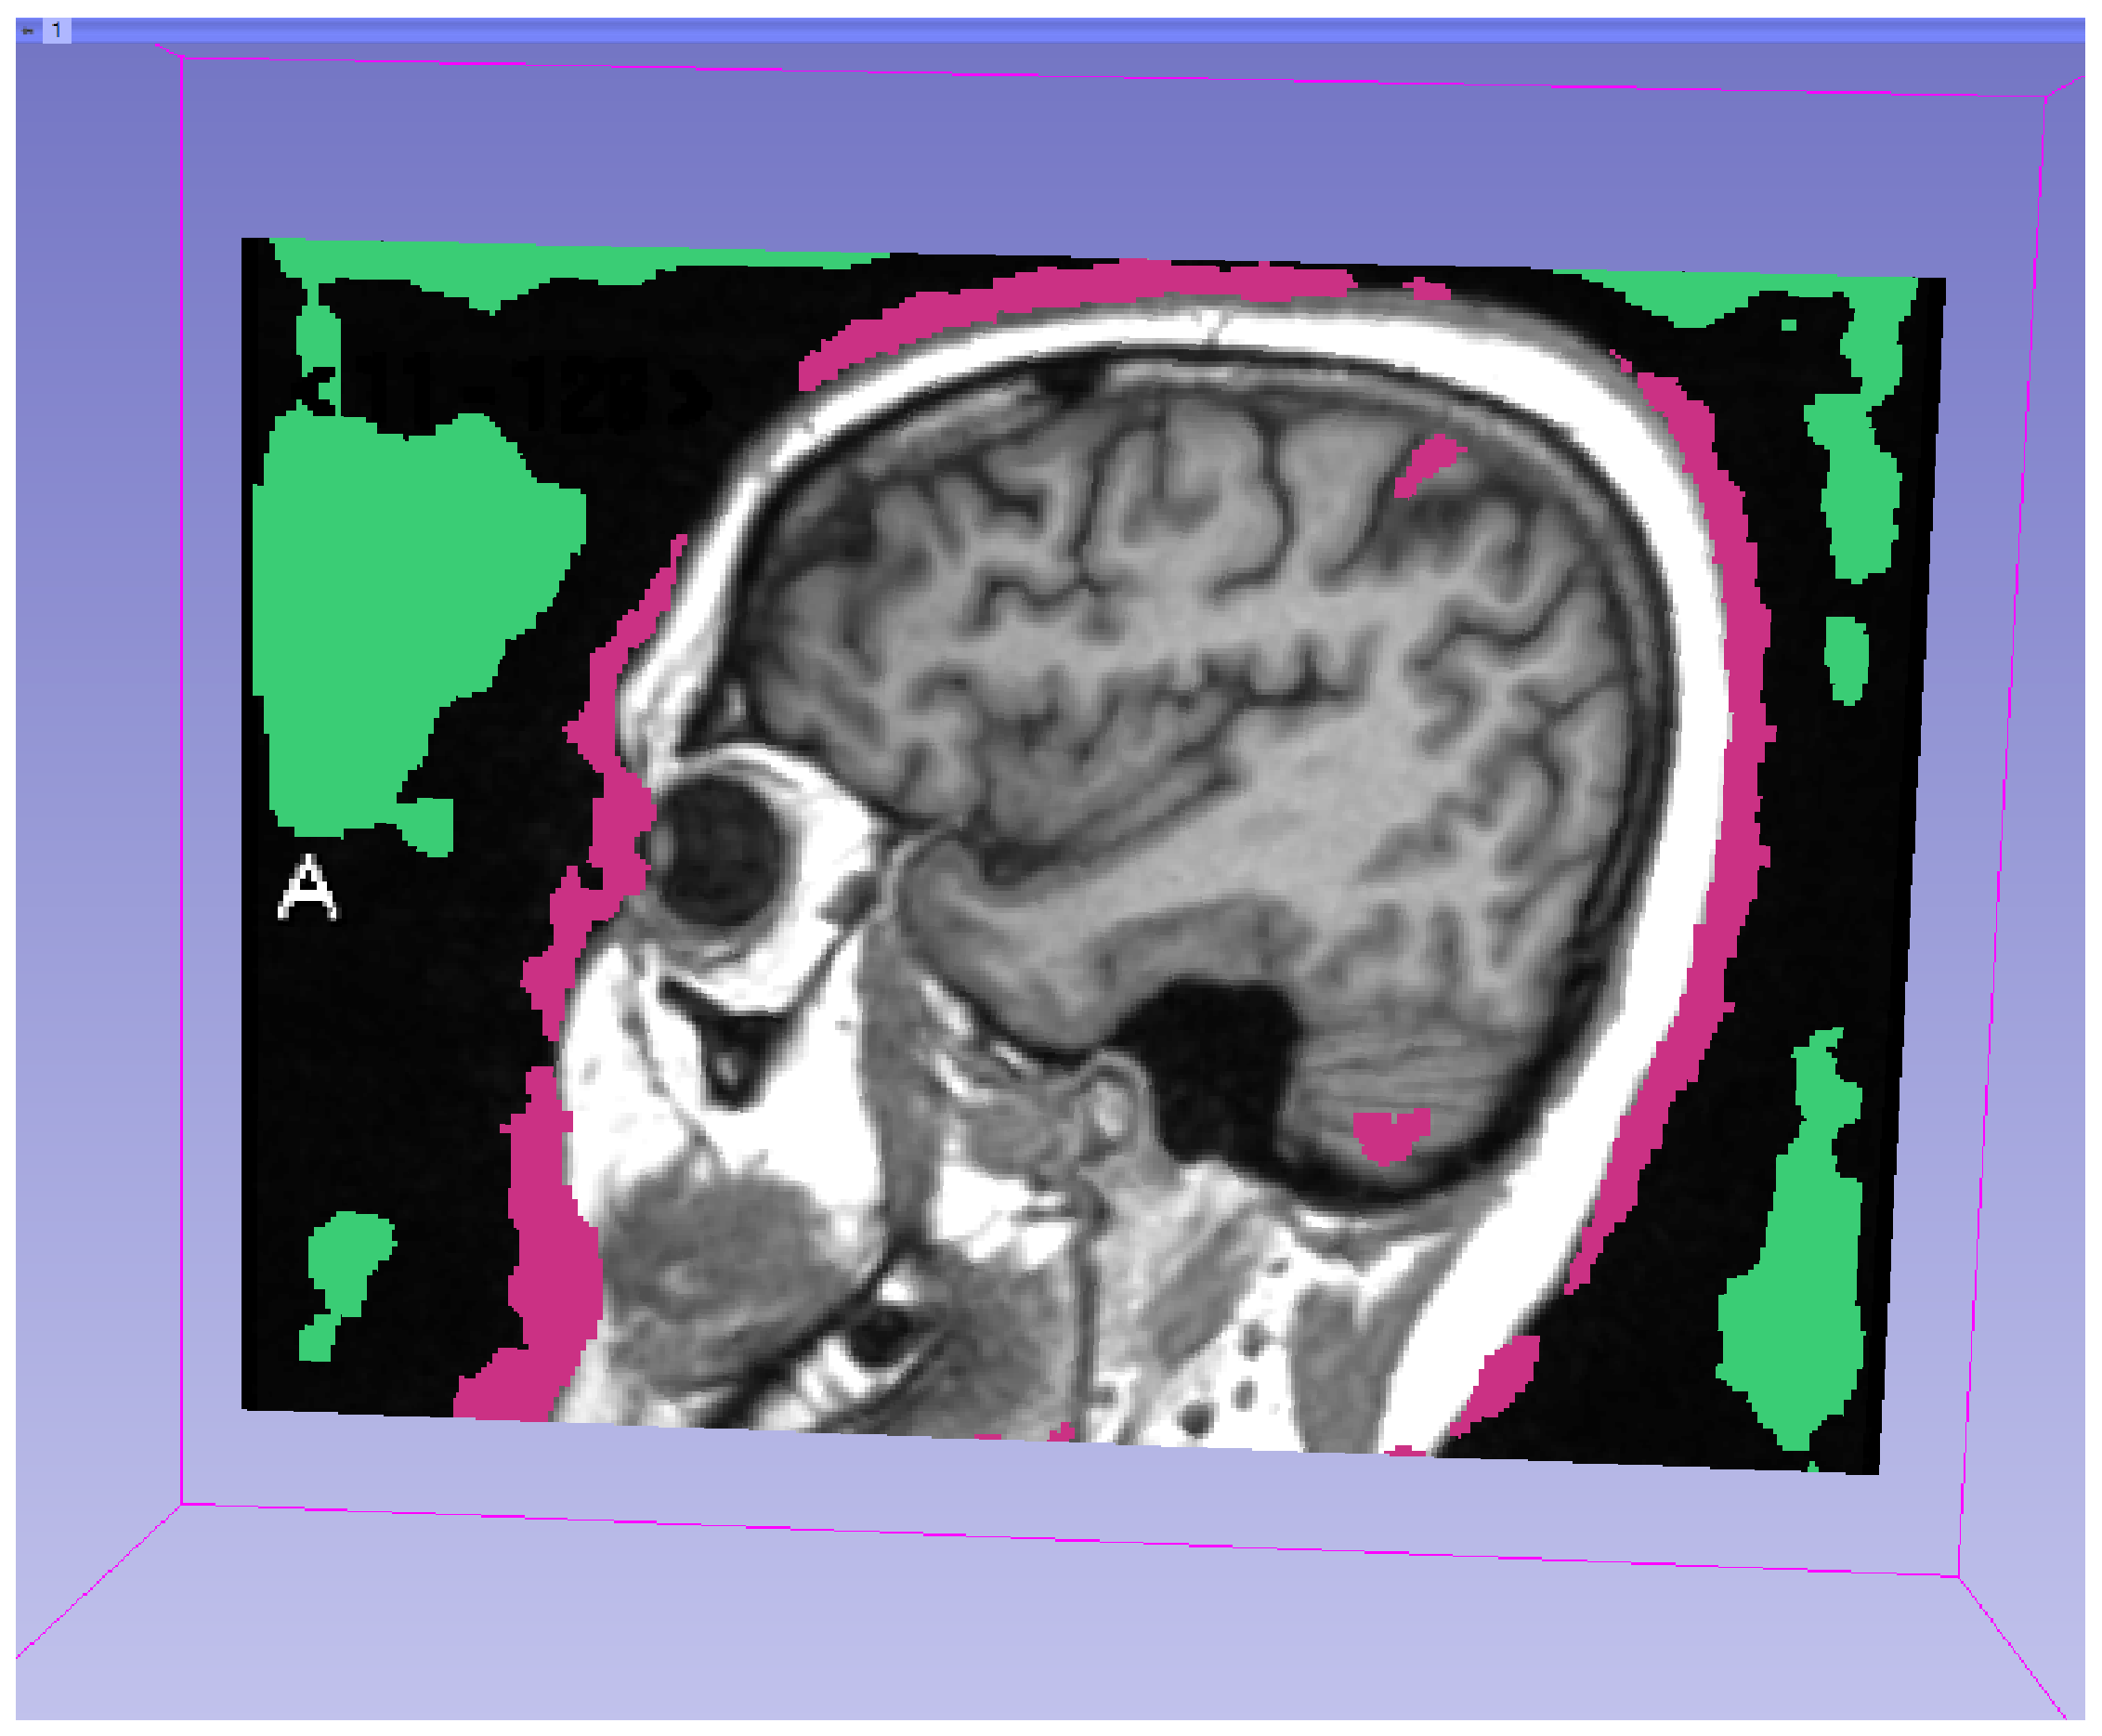
\includegraphics[scale=0.2]{/experiment_CL_P1/CL_Tensor_Sagittal.eps}
  \caption{Tensor-based method. Patient 1: Sagittal plane}
  \label{CL_TSagittal}
\end{figure}


\subsection{Patient 2}
The differences in this patient, if actually present, are really
small. 

\subsubsection{Voxel-based Method}
The voxel-based method shows small differences near the corpus
callosum on the three planes; this differences, accourding to the
medical expert, might be real because this is a very common area
affected by trauma.\\

The registration method used was \textit{Affine registration}.

\begin{figure}[H]
  \centering
  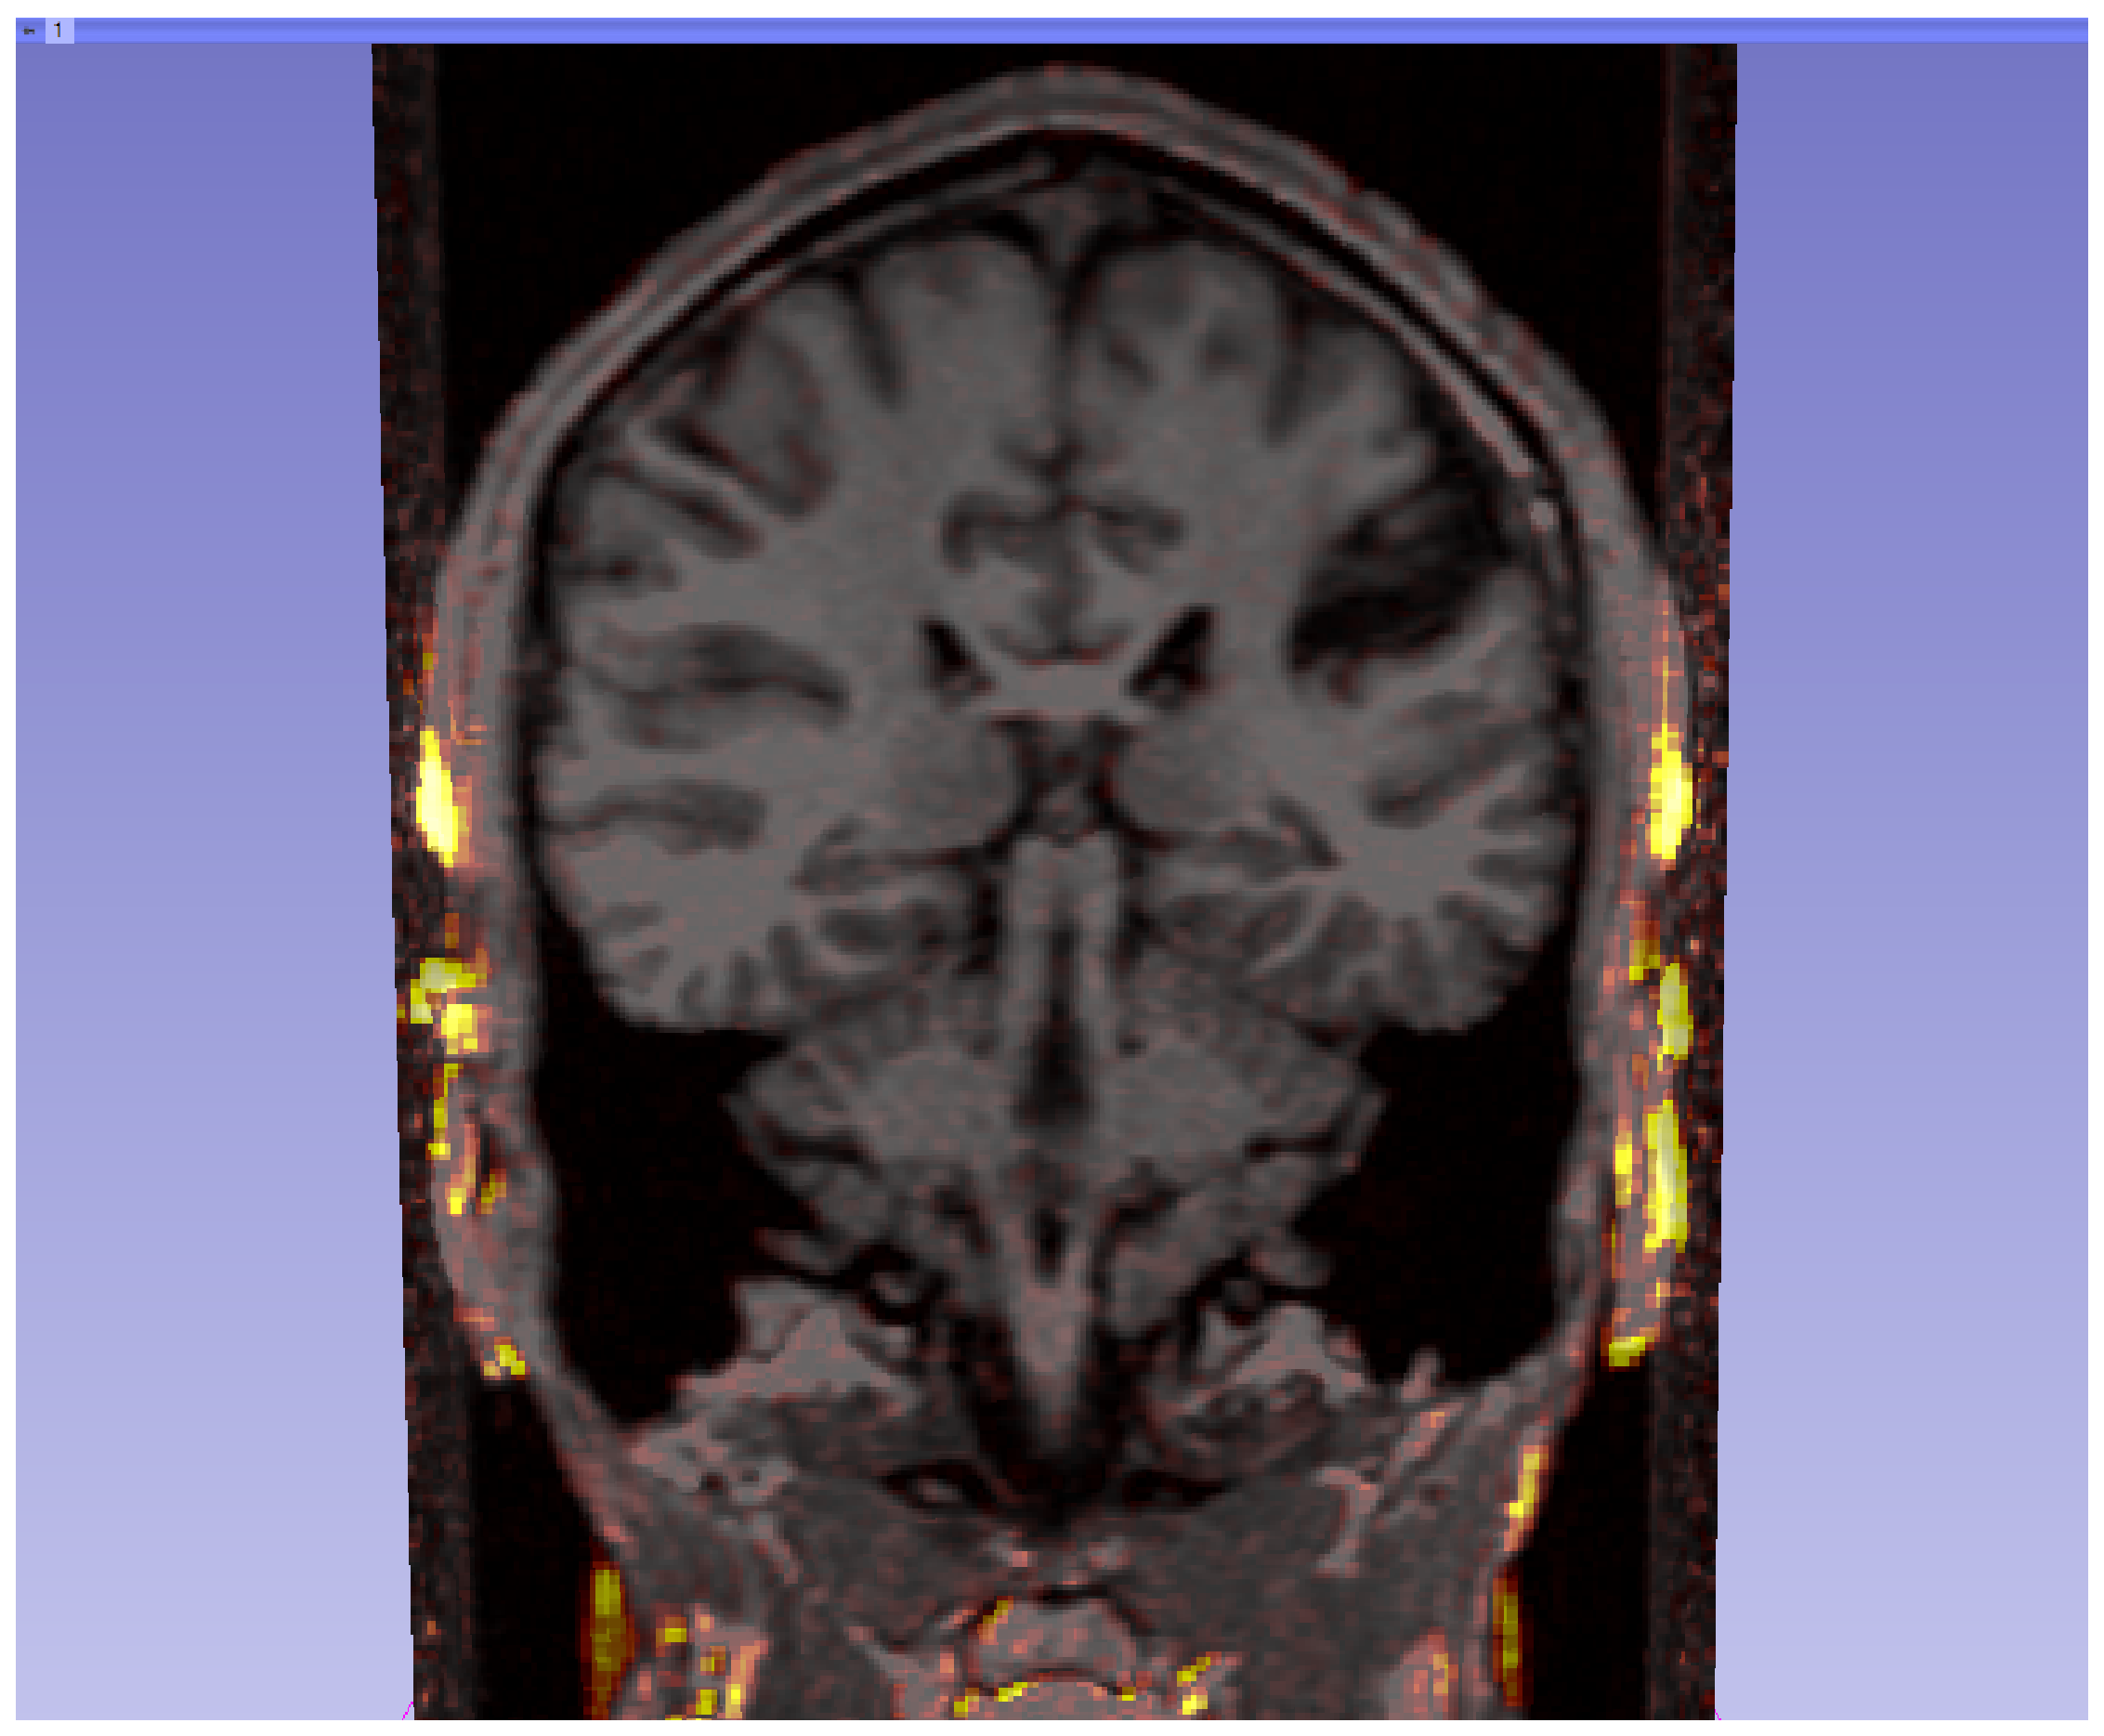
\includegraphics[scale=0.2]{/experiment_PB_P2/PB_Coronal.eps}
  \caption{Voxel-based method. Patient 2: Coronal plane}
  \label{PB_Coronal}
\end{figure}

\begin{figure}[H]
  \centering
  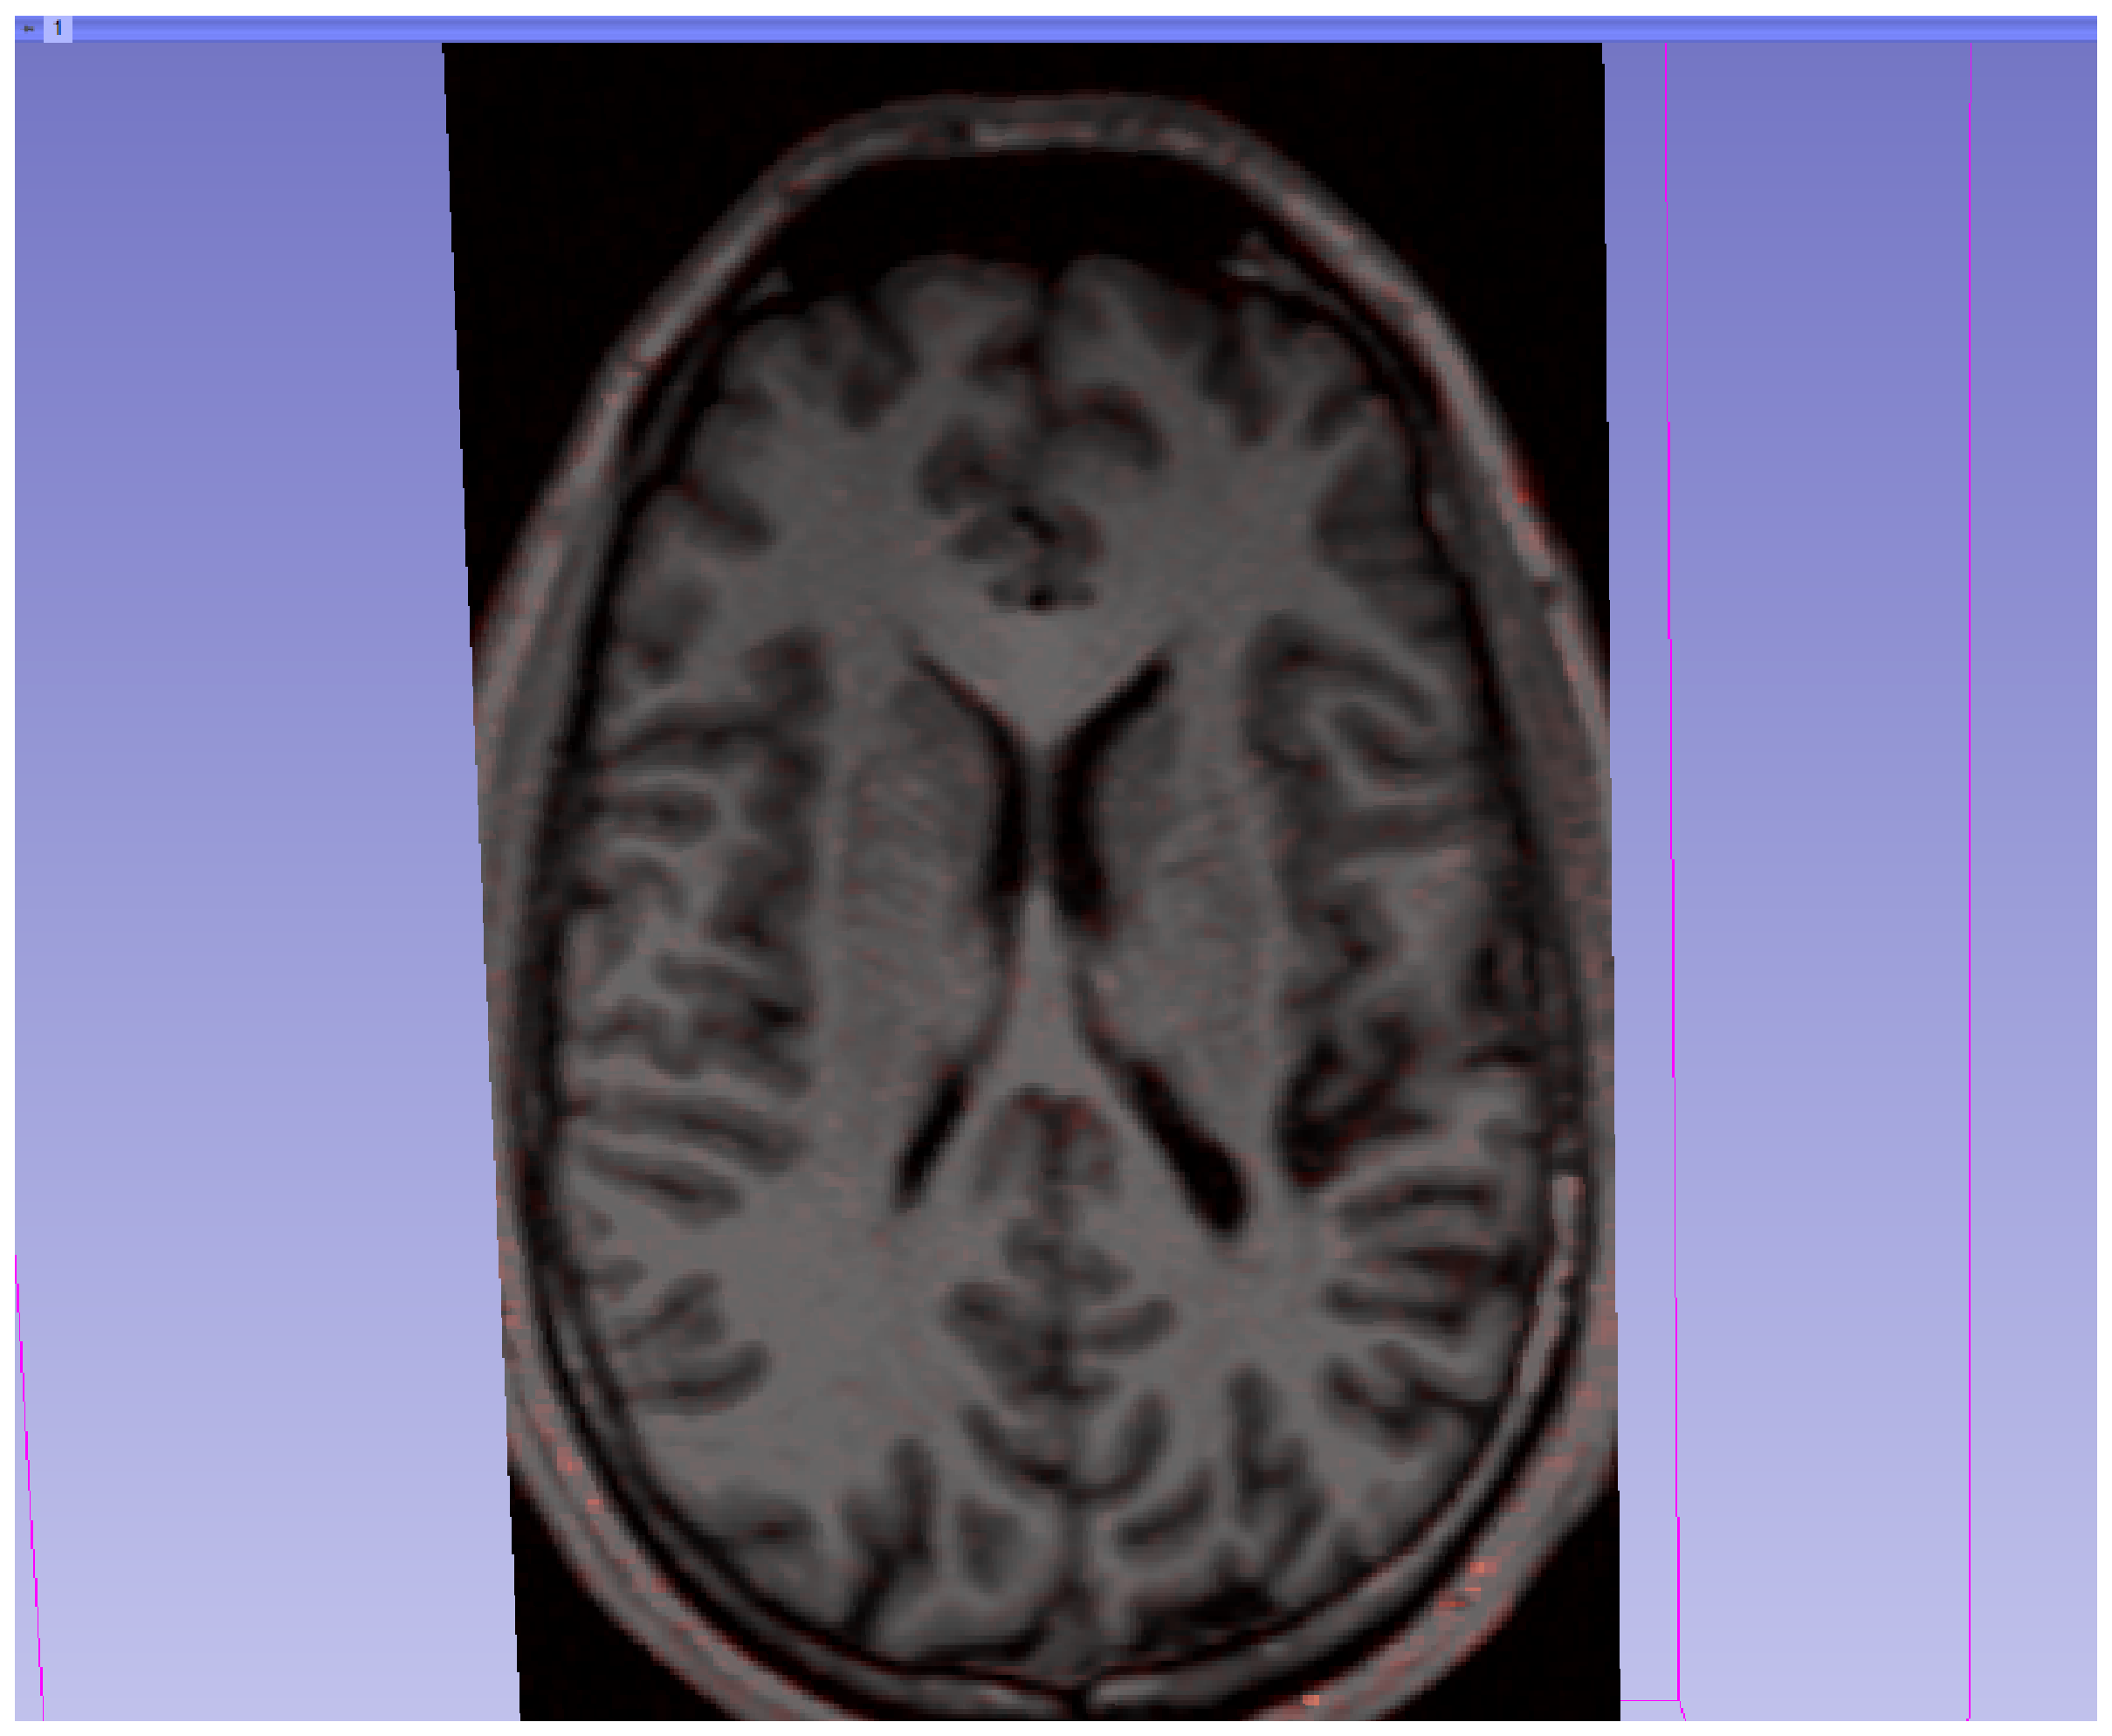
\includegraphics[scale=0.2]{/experiment_PB_P2/PB_Traversal.eps}
  \caption{Voxel-based method. Patient 2: Traversal plane}
  \label{PB_Traversal}
\end{figure}

\begin{figure}[H]
  \centering
  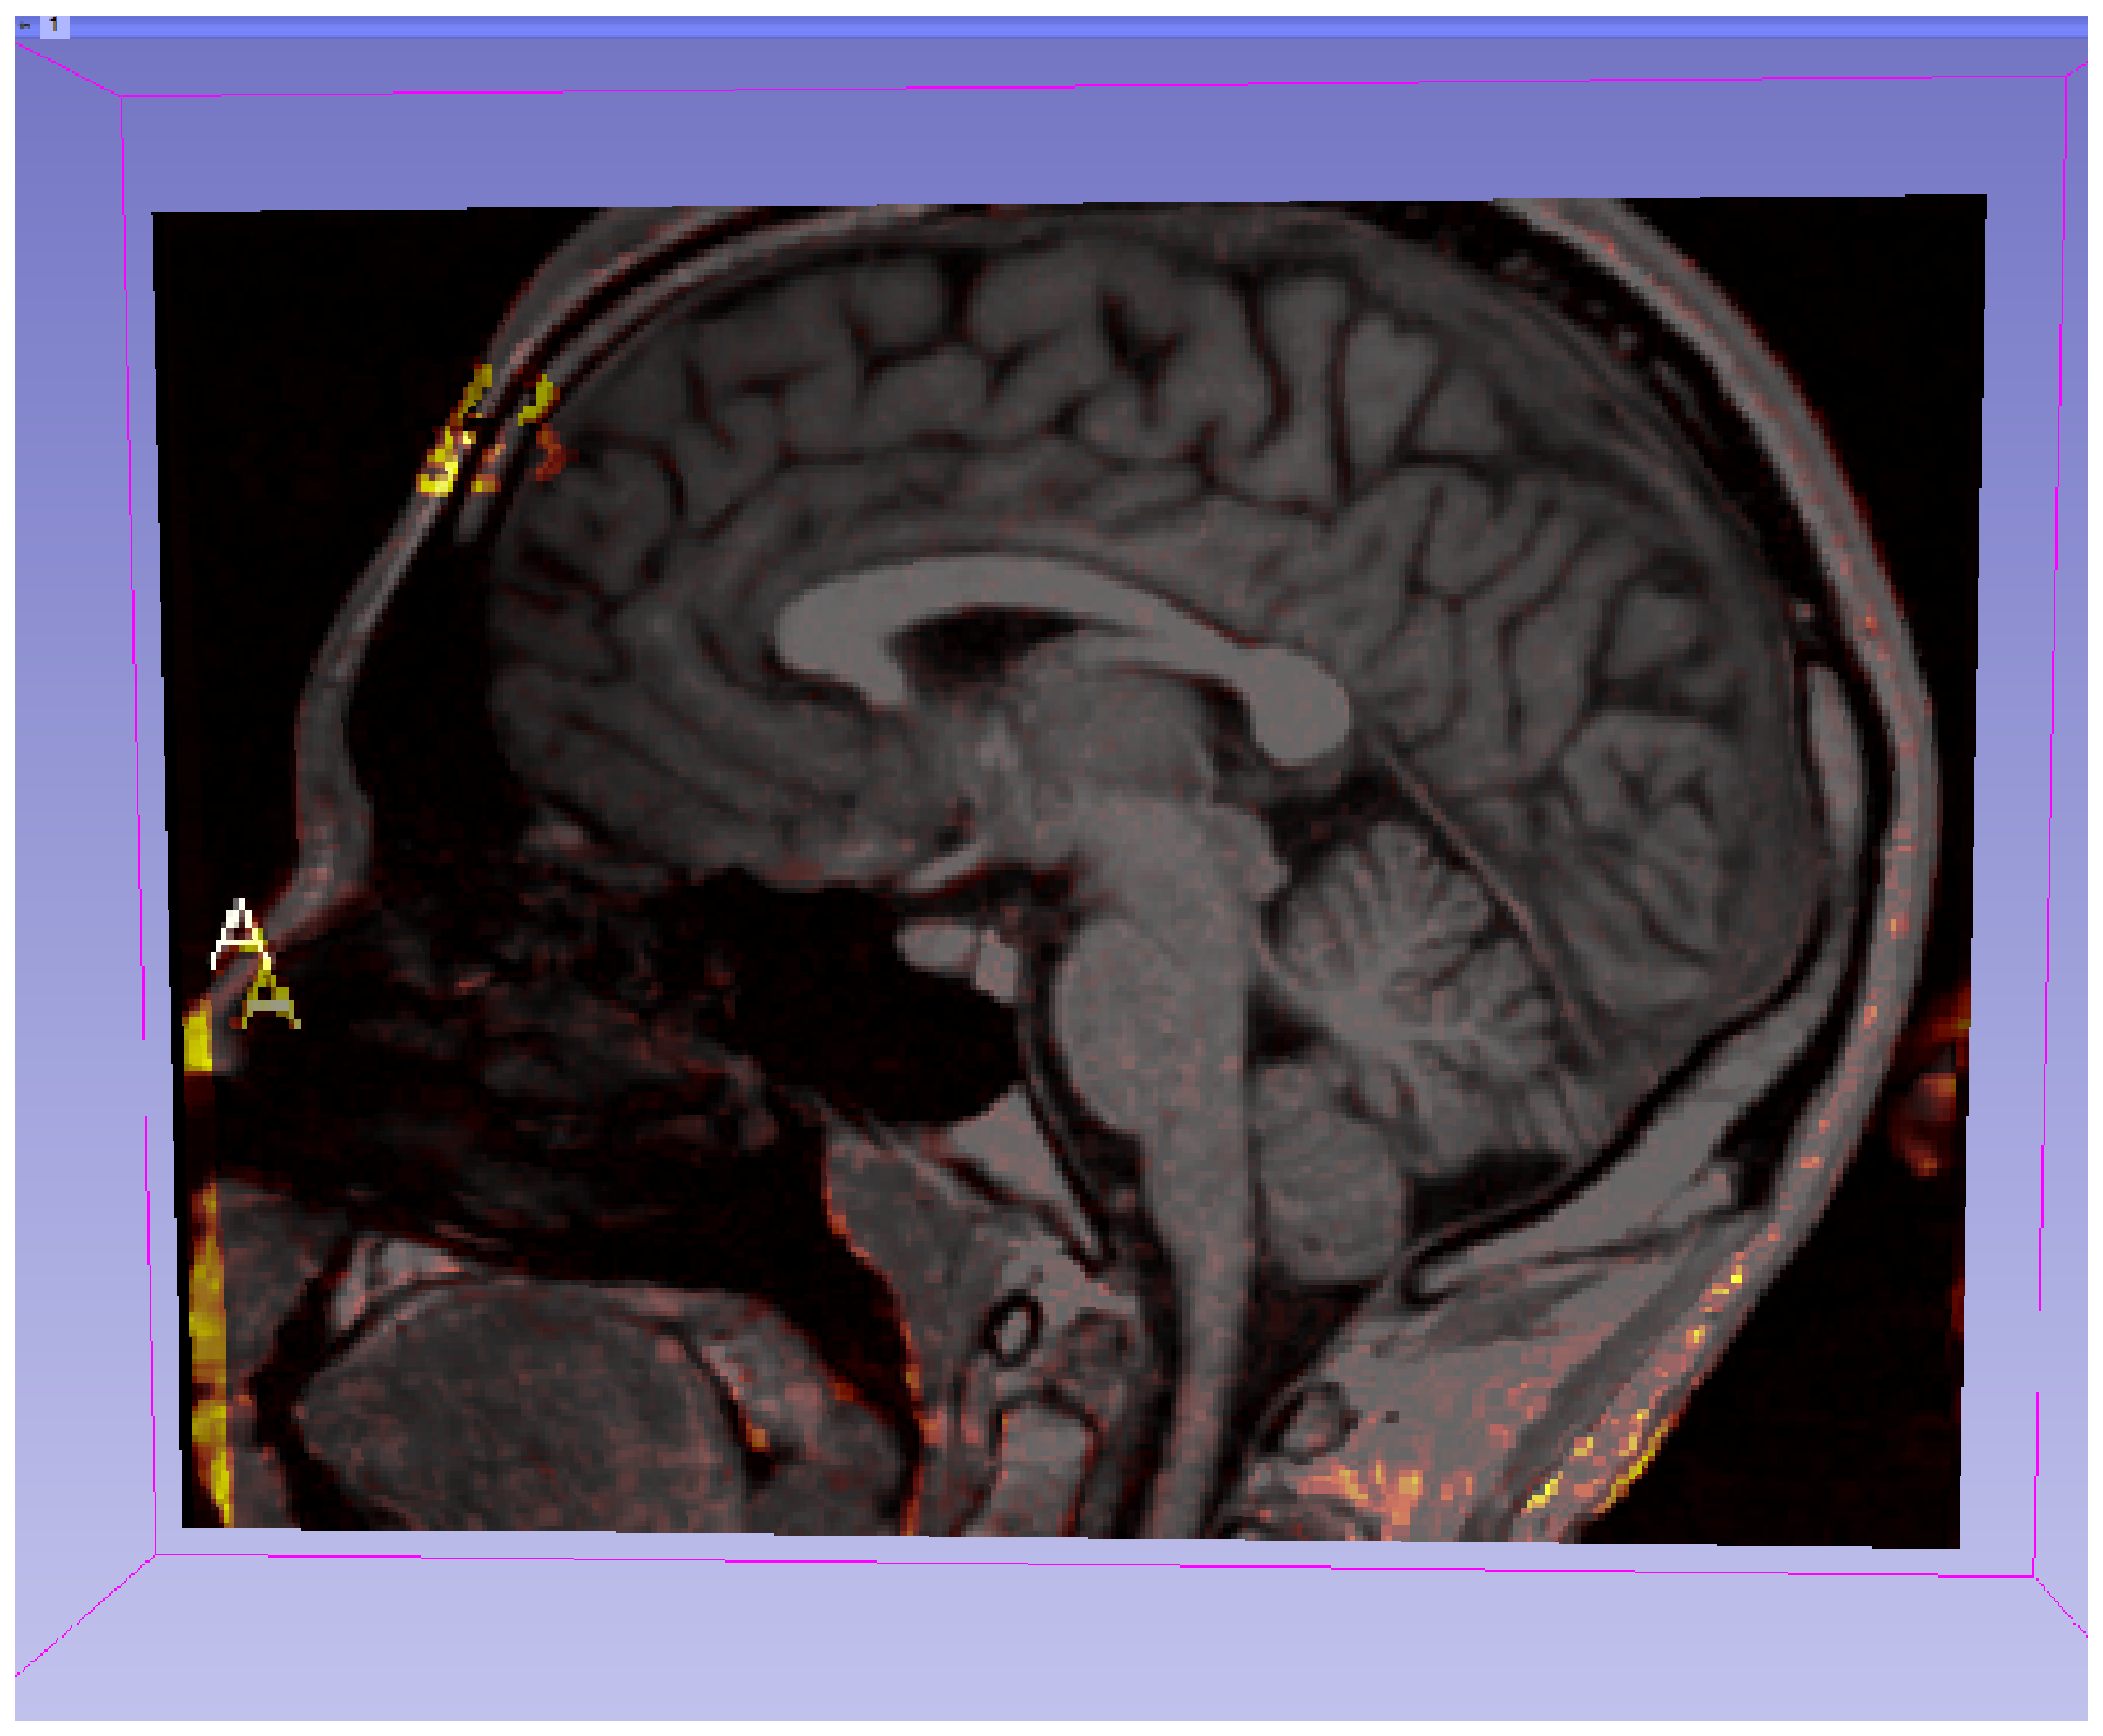
\includegraphics[scale=0.2]{/experiment_PB_P2/PB_Sagittal.eps}
  \caption{Voxel-based method. Patient 2: Sagittal plane}
  \label{PB_Sagittal}
\end{figure}


\subsubsection{Tensor-based Method}
The tensor-base method doesn't find the same differences in the corpus
callosum as the previous method. With the usual percentage values
(from $70\%$ to $80\%$ for both growth and shrinkage), the method almost
doesn't find any differences. 

In order to show some of the possible places where the method shows
some type of differences, the value of the shrinkage percentage was
increased until $88\%$. Given this, the pink areas shown are not
necessarily real differences.\\

Parameters used:
\begin{description}
\item \textit{Deformation field smoothing sigma:} 2.5
\item \textit{Shrinkage percentage:} 80
\item \textit{Growth percentage:} 88
\end{description}

\begin{figure}[H]
  \centering
  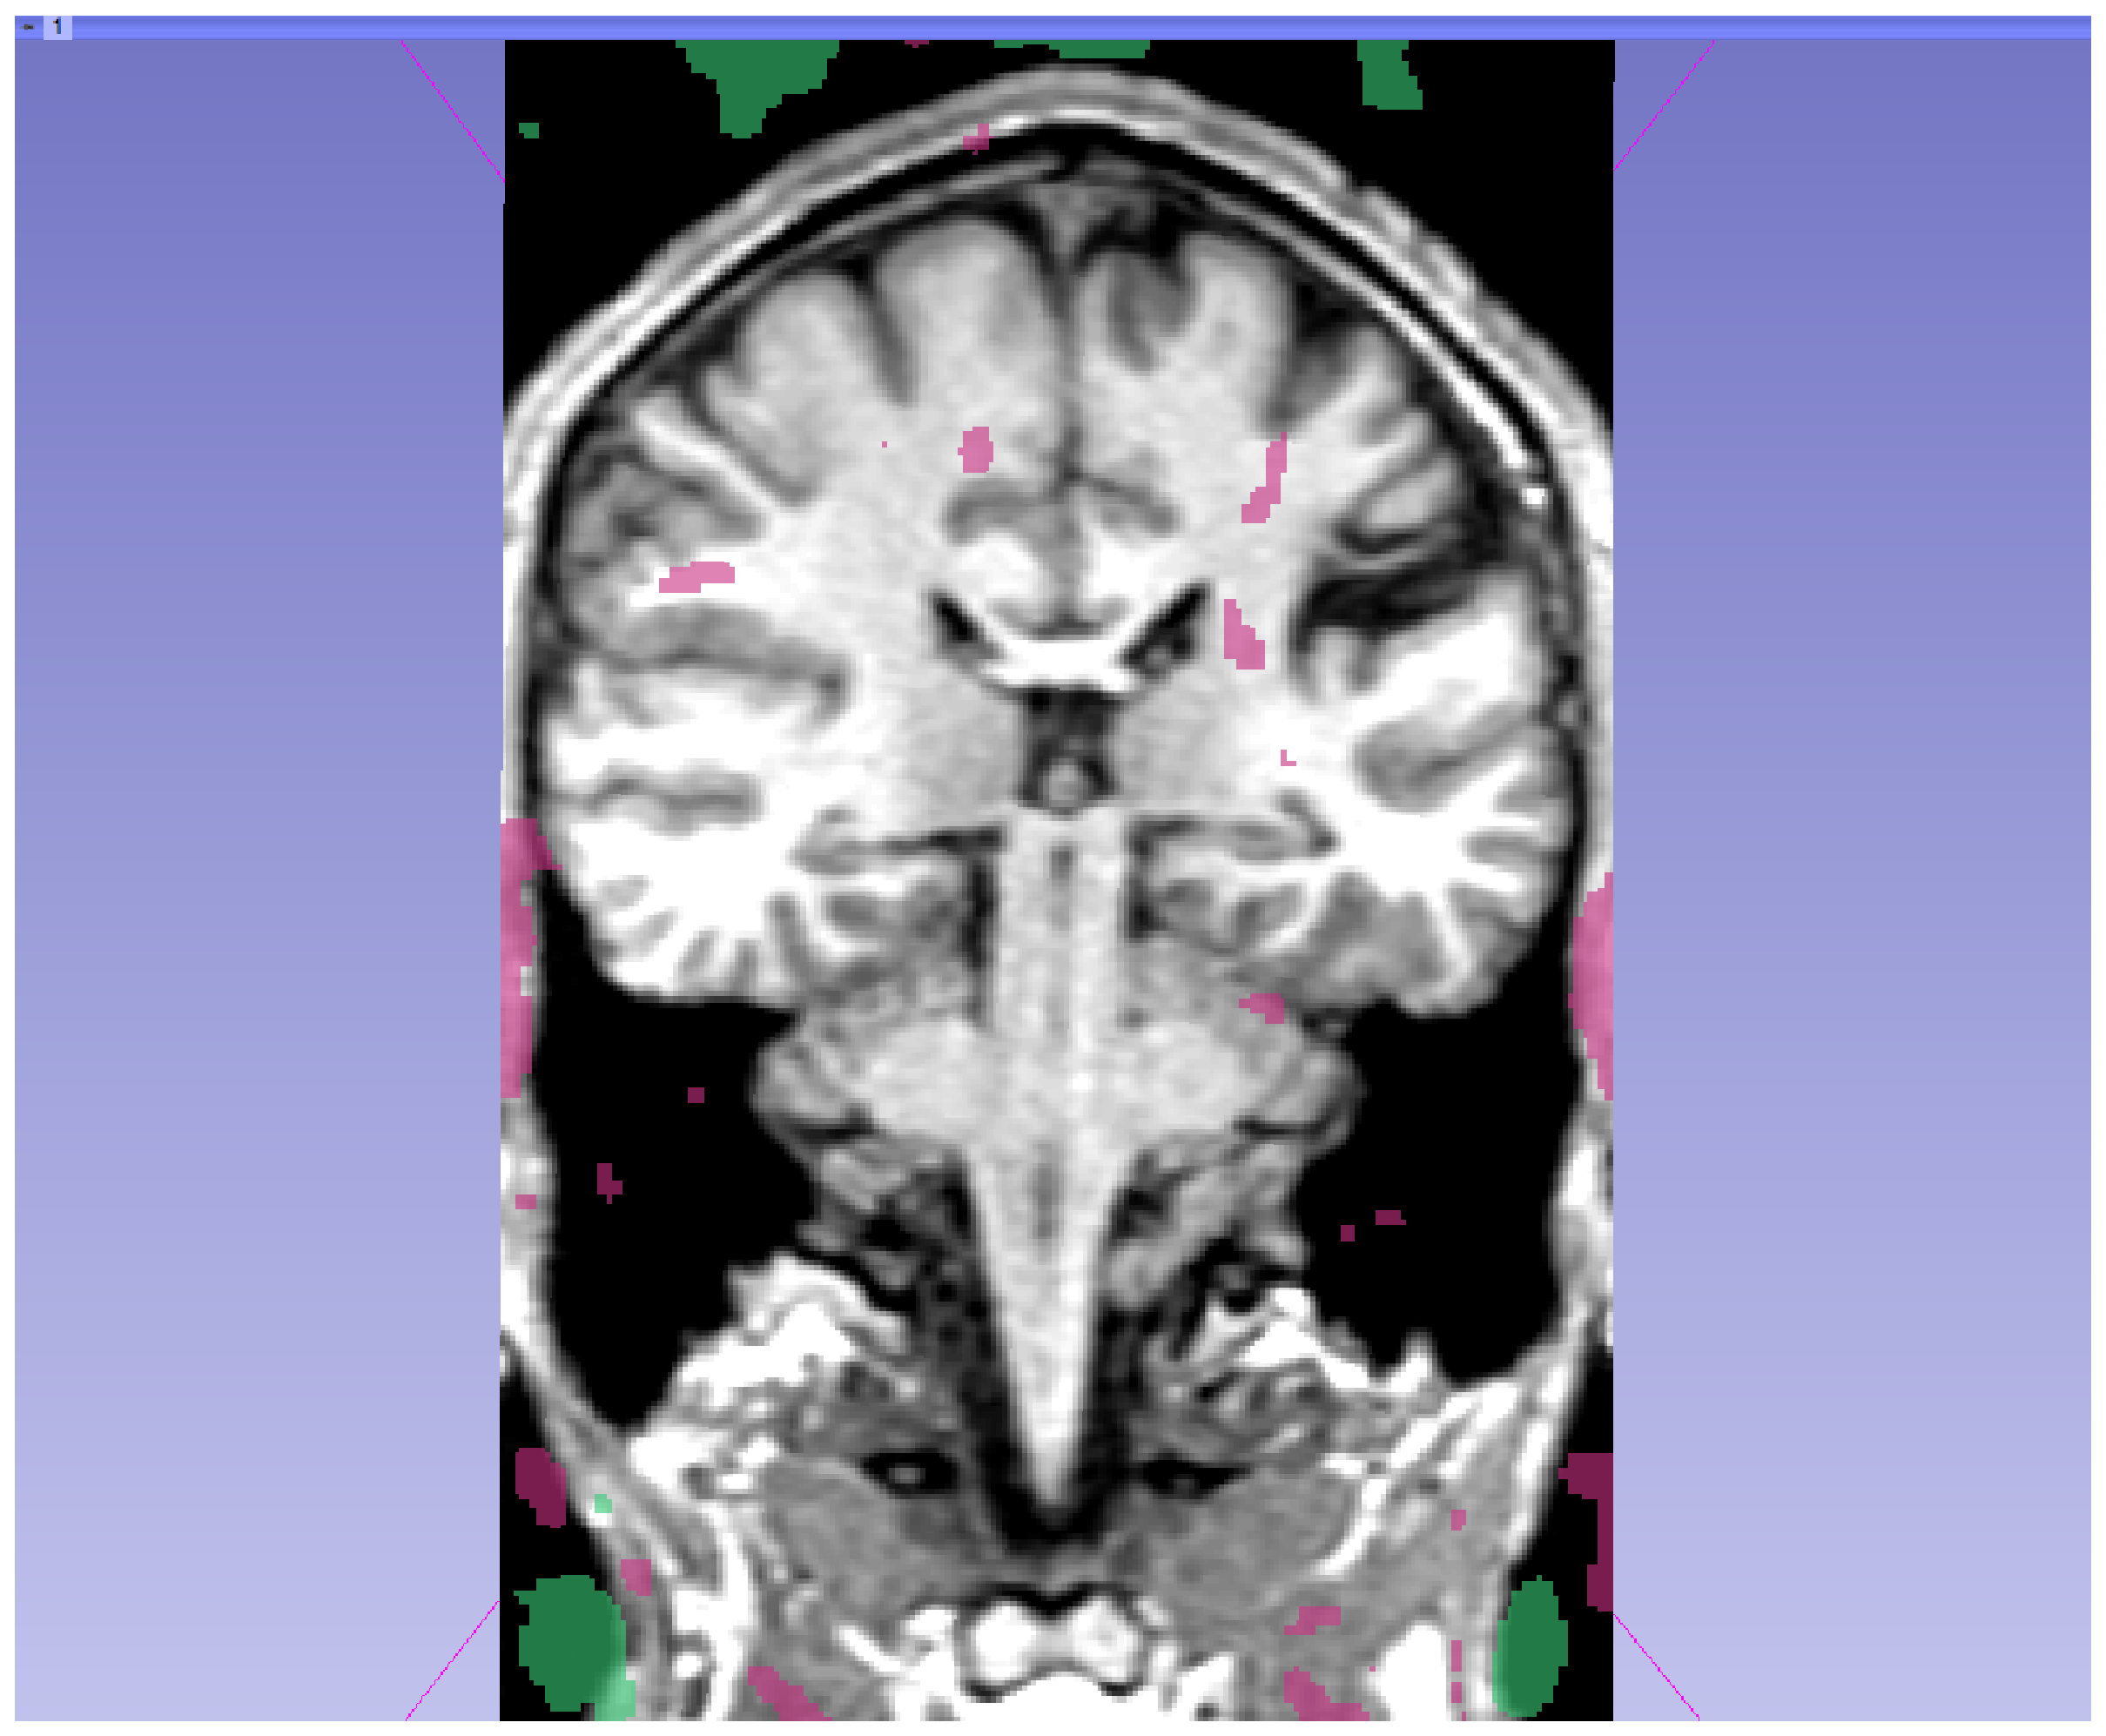
\includegraphics[scale=0.2]{/experiment_PB_P2/PB_Tensor_Coronal.eps}
  \caption{Tensor-based method. Patient 2: Coronal plane}
  \label{PB_TCoronal}
\end{figure}

\begin{figure}[H]
  \centering
  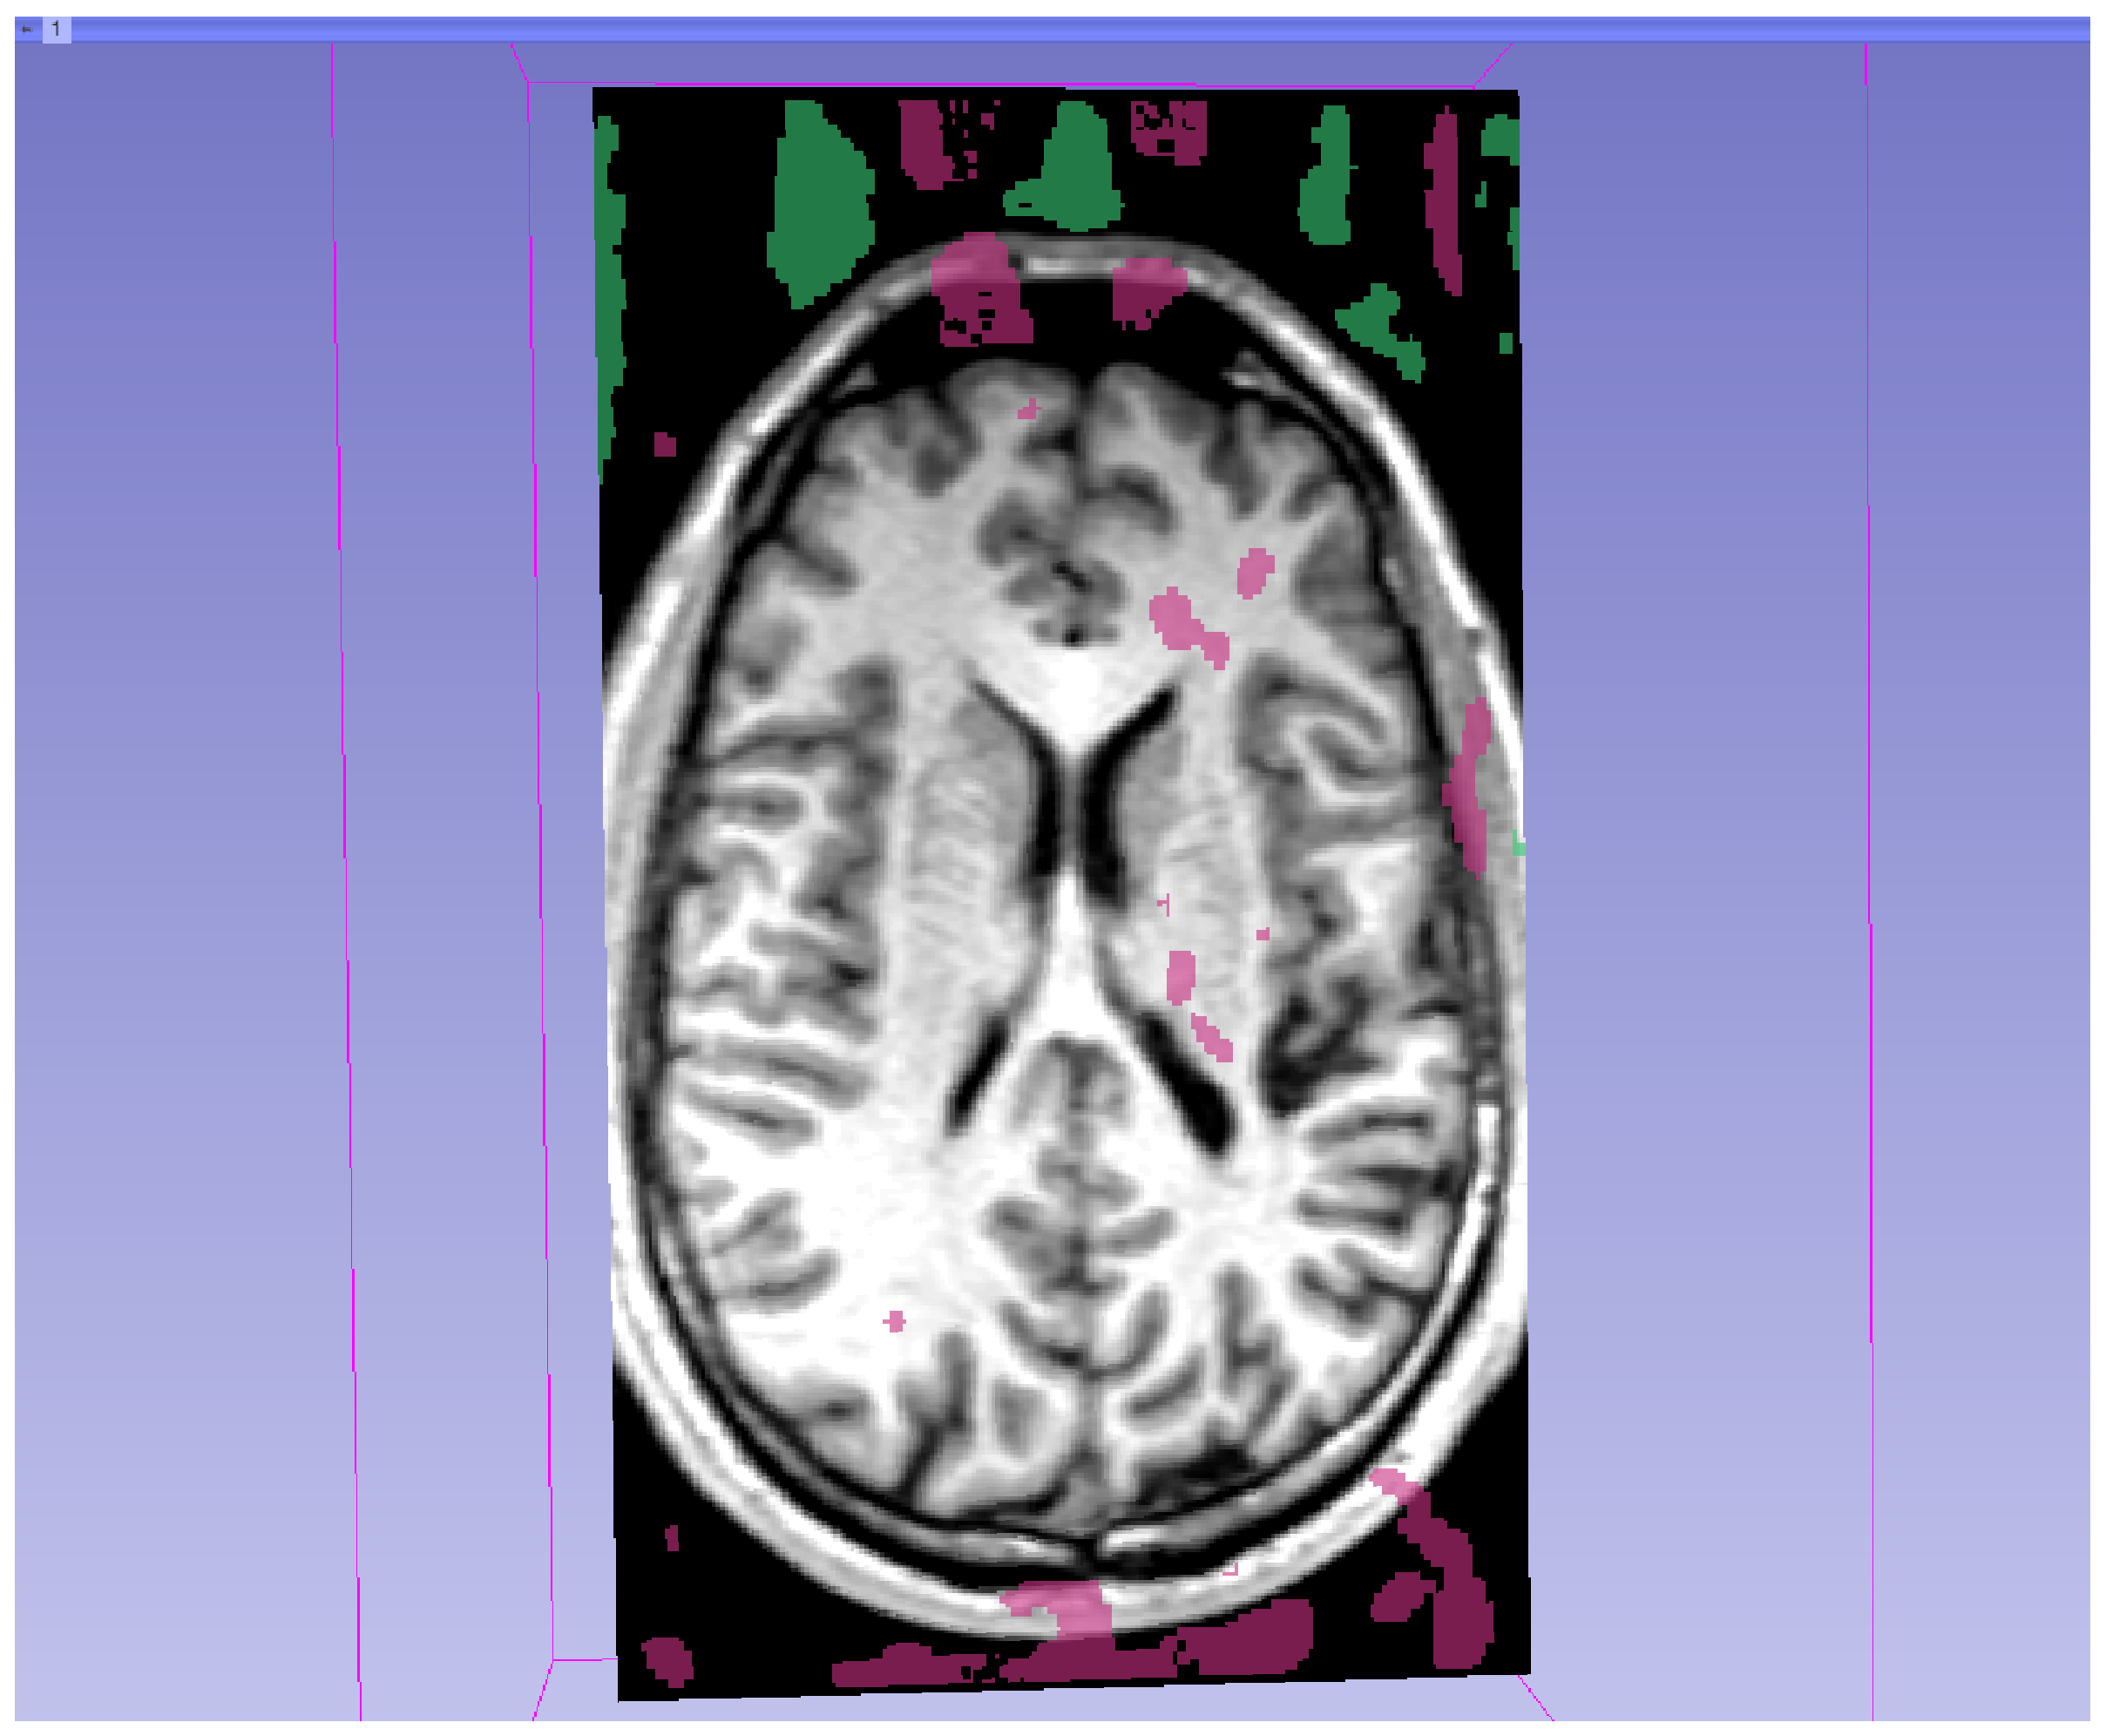
\includegraphics[scale=0.2]{/experiment_PB_P2/PB_Tensor_Traversal.eps}
  \caption{Tensor-based method. Patient 2: Traversal plane}
  \label{PB_TTraversal}
\end{figure}

\begin{figure}[H]
  \centering
  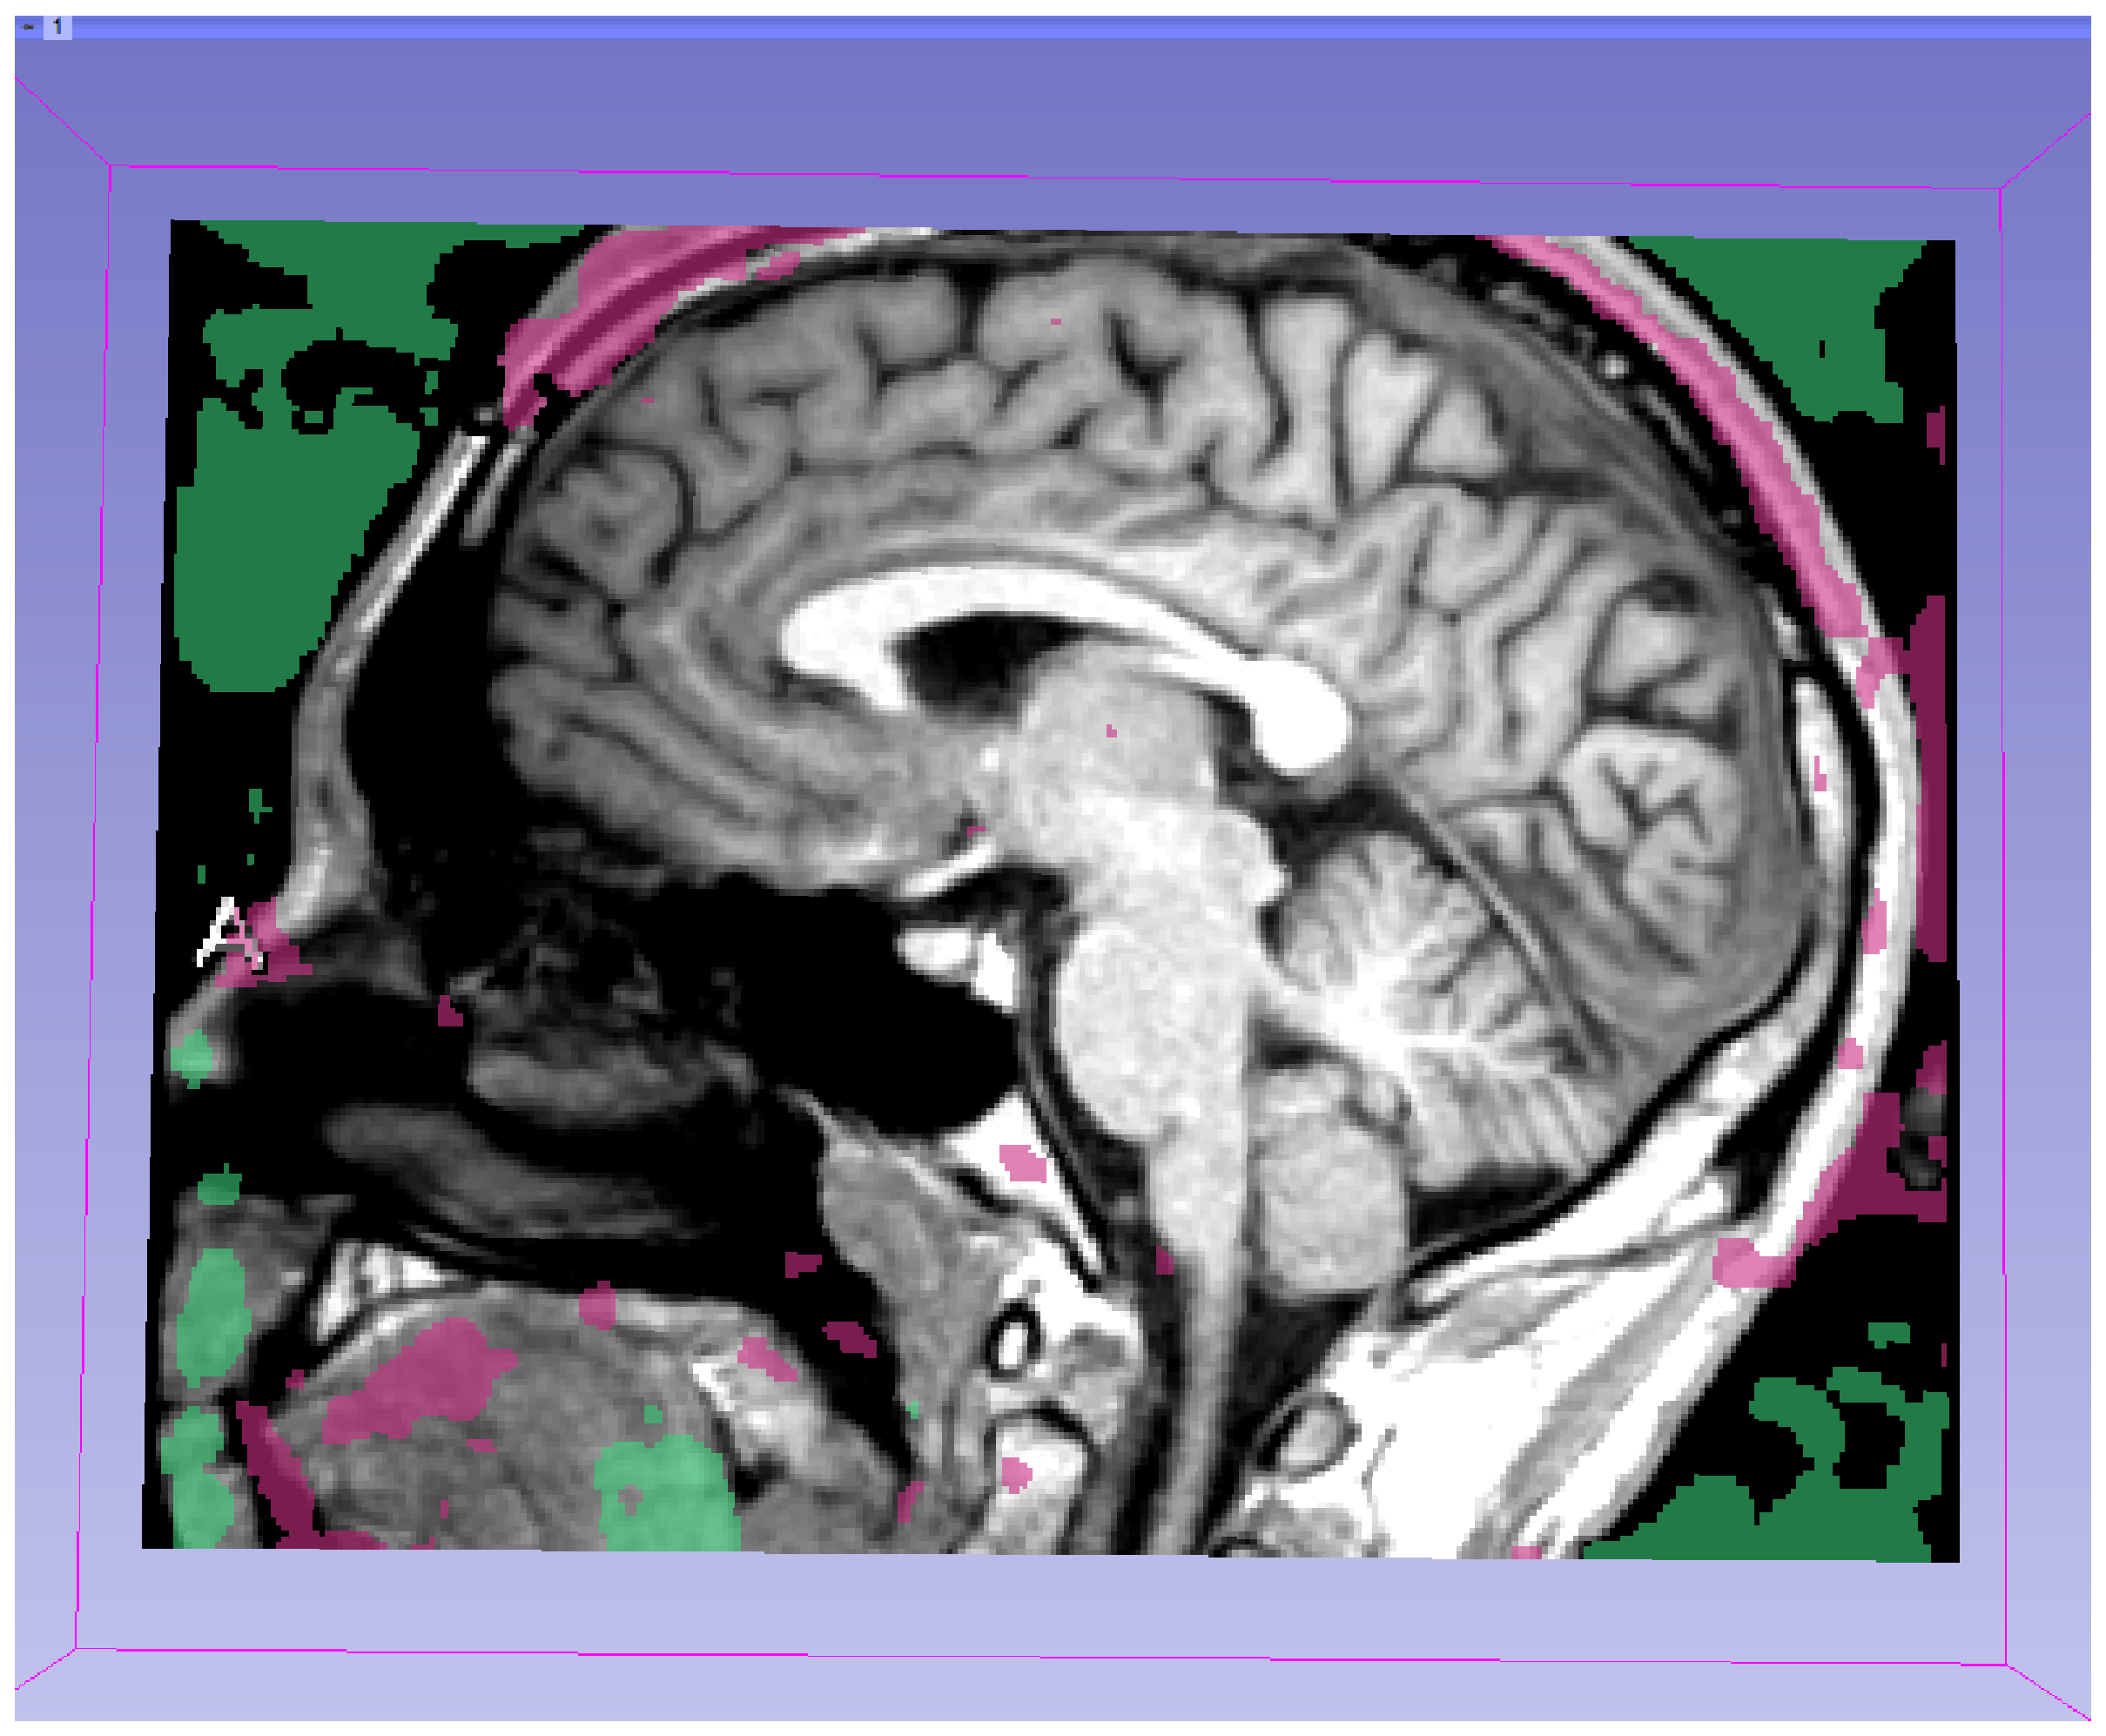
\includegraphics[scale=0.2]{/experiment_PB_P2/PB_Tensor_Sagittal.eps}
  \caption{Tensor-based method. Patient 2: Sagittal plane}
  \label{PB_TSagittal}
\end{figure}


\subsection{Patient 3}
This patient had a medical condition for which it has had two
surgeries performed. A tumor, located on the right hemisphere of the
frontal lobe, was removed during the first surgery. The MRIs used
during this experiment were taken before and after the second surgery,
in which a second growth was removed located the same area.


\subsubsection{Voxel-based Method}
The method shows the expected differences in the right hemisphere of
the frontal lobe of the brain. It also shows some size differences
especially in the lower parietal lobe, which can be observed in image
\ref{B2_Traversal1}.\\

The registration method used was \textit{Affine registration}.

\begin{figure}[H]
  \centering
  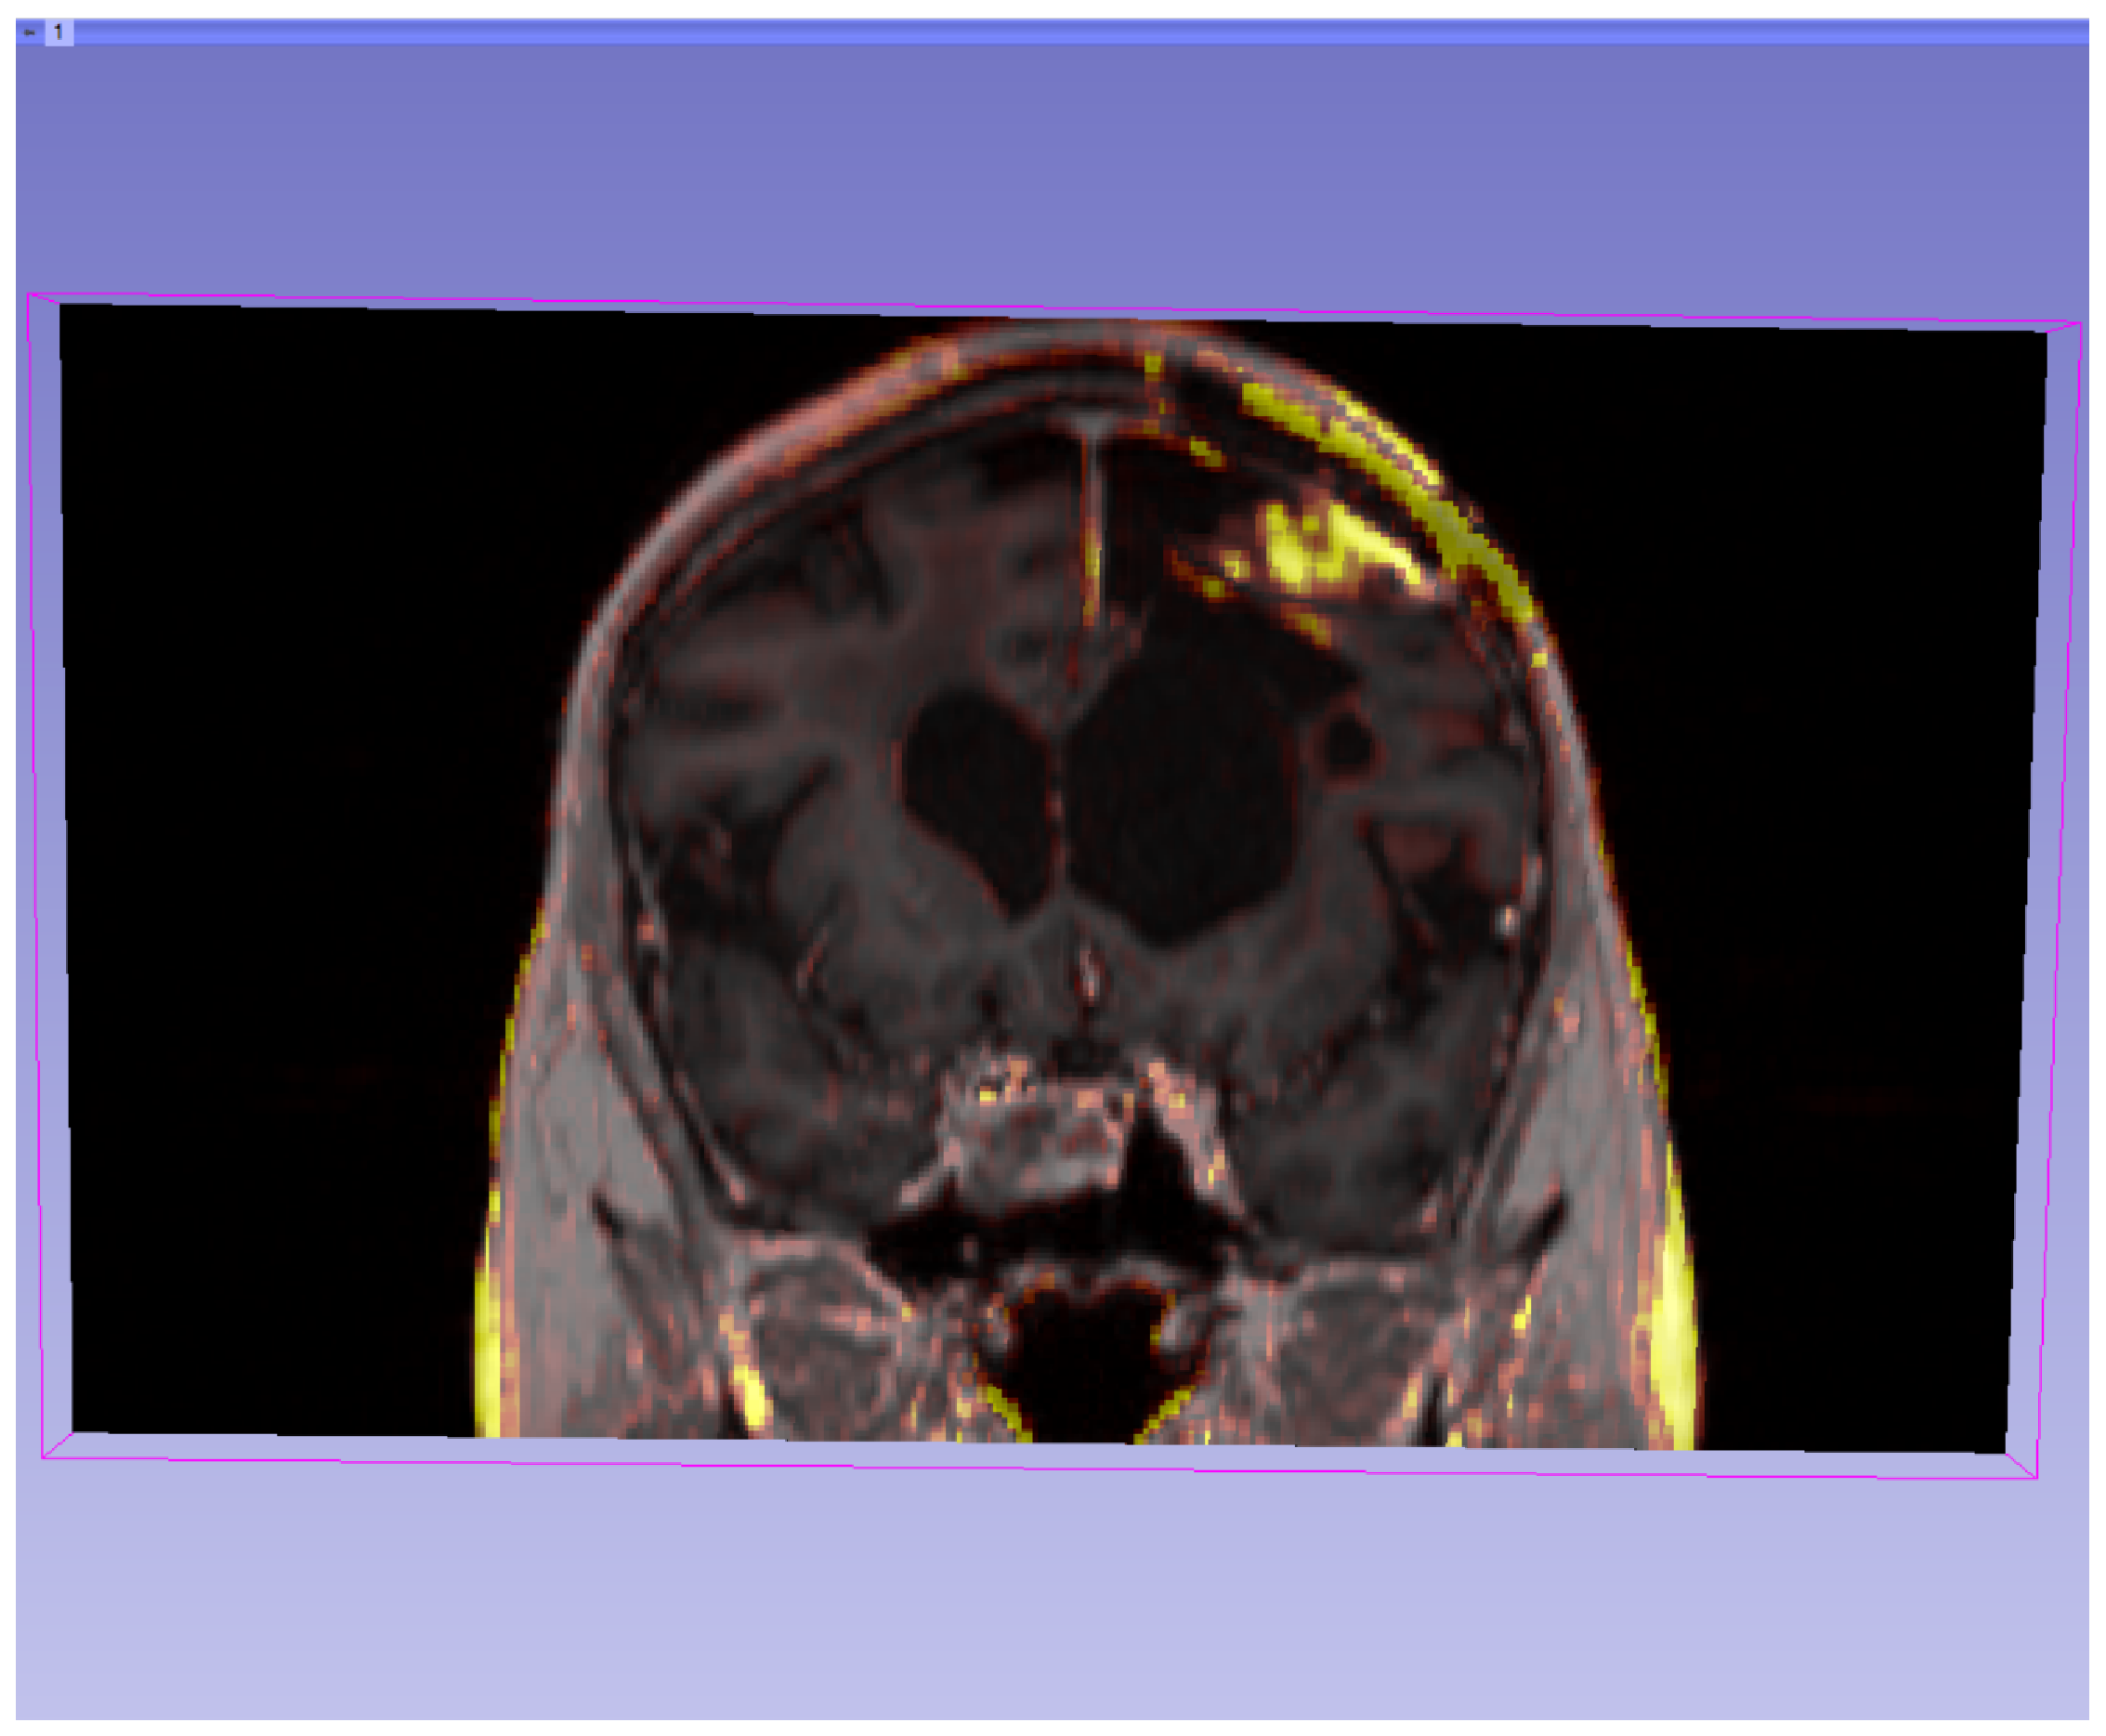
\includegraphics[scale=0.2]{/experiment_B2_P3/B2_Coronal.eps}
  \caption{Voxel-based method. Patient 3: Coronal plane}
  \label{B2_Coronal}
\end{figure}

\begin{figure}[H]
  \centering
  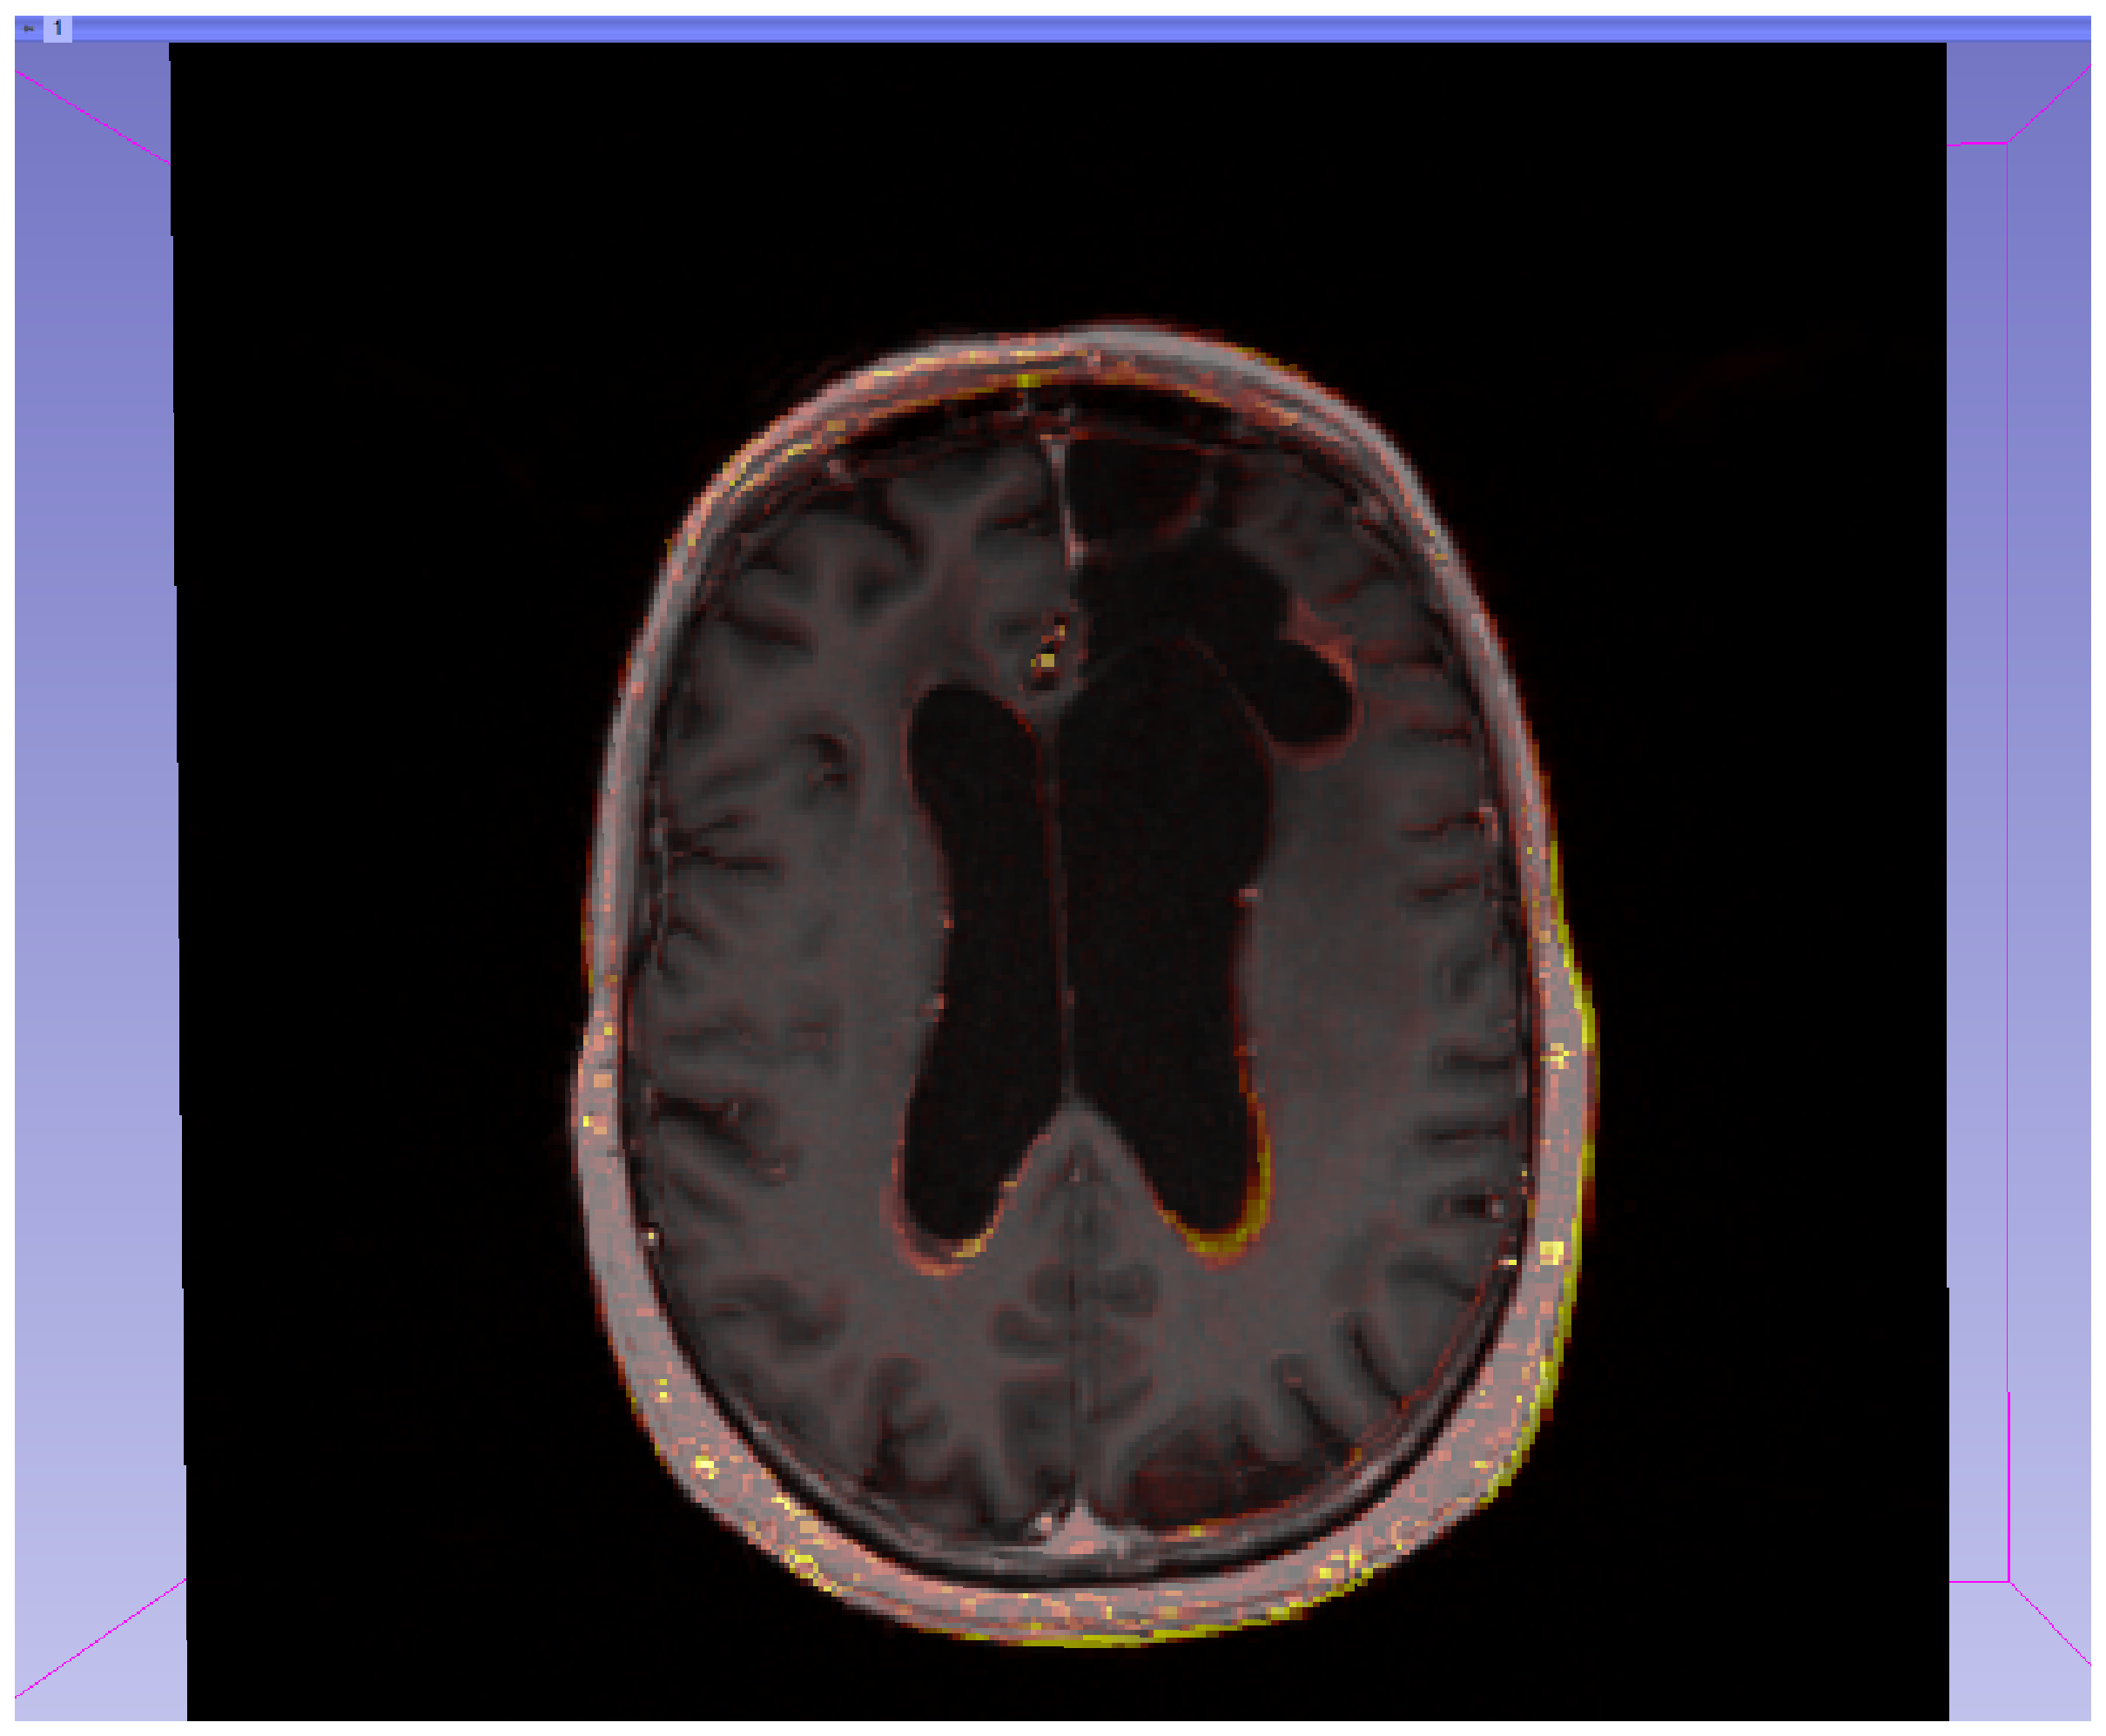
\includegraphics[scale=0.2]{/experiment_B2_P3/B2_Traversal1.eps}
  \caption{Voxel-based method. Patient 3: Traversal plane}
  \label{B2_Traversal1}
\end{figure}

\begin{figure}[H]
  \centering
  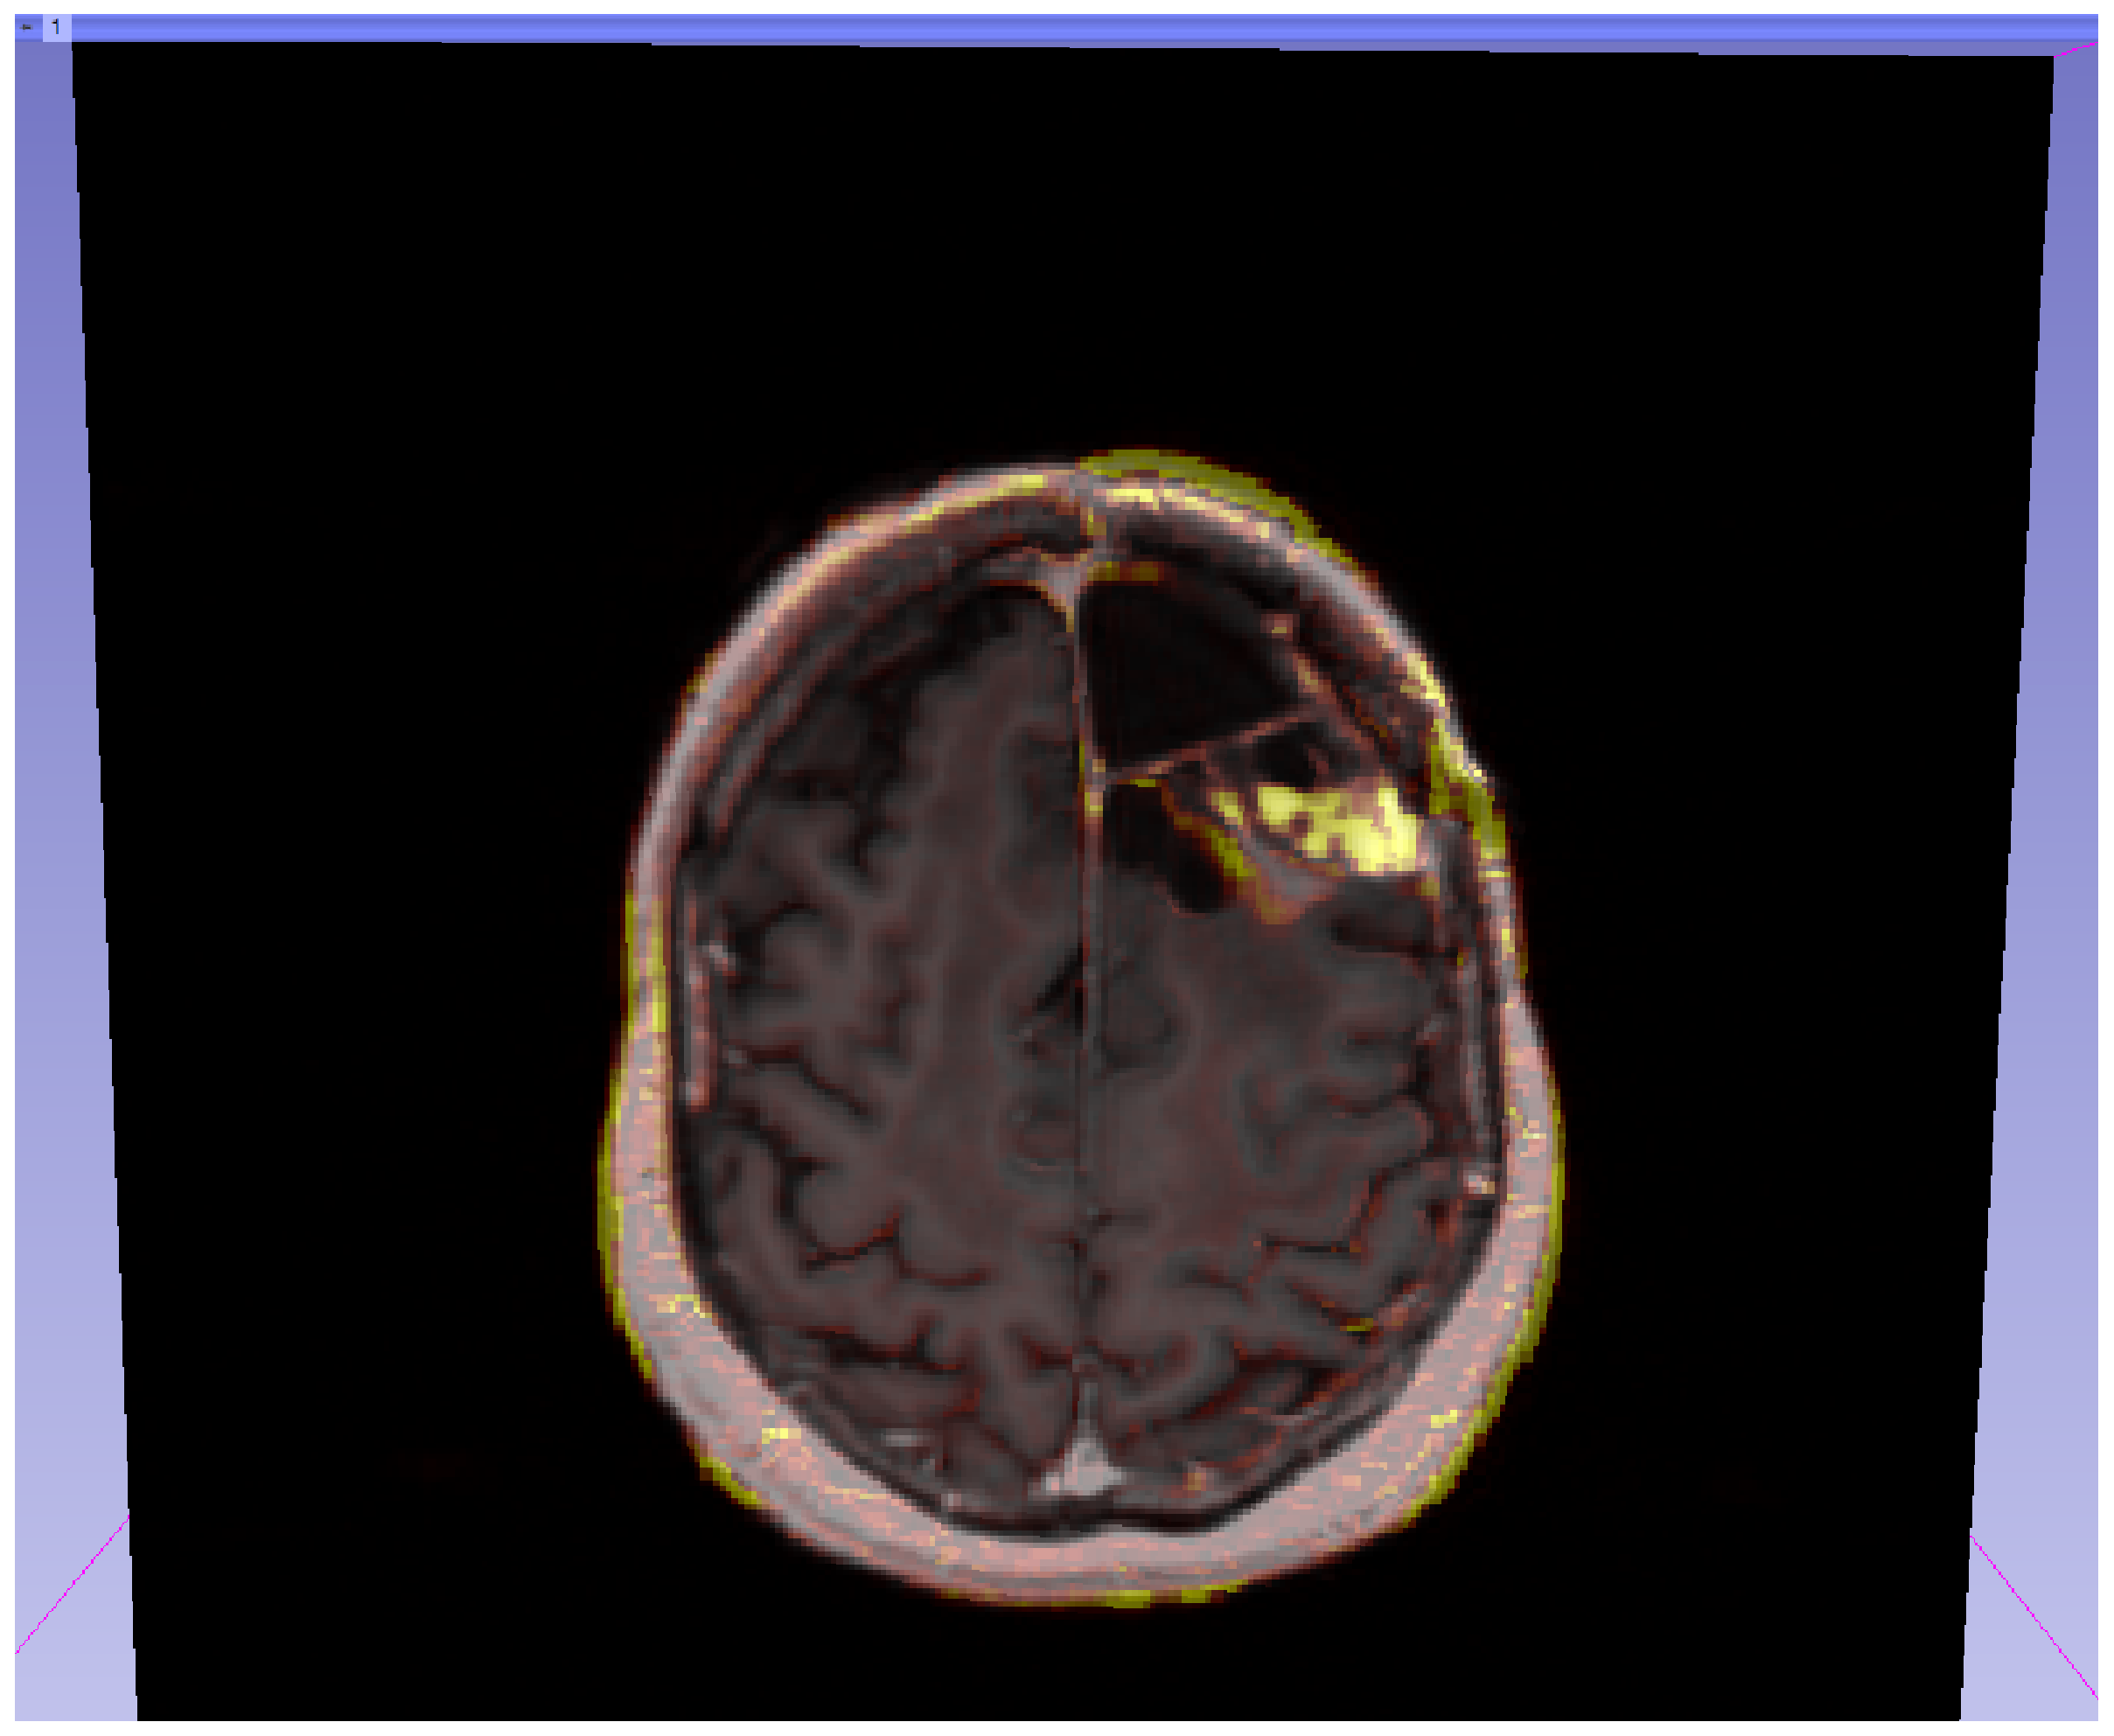
\includegraphics[scale=0.2]{/experiment_B2_P3/B2_Traversal2.eps}
  \caption{Voxel-based method. Patient 3: Upper traversal plane}
  \label{B2_Traversal2}
\end{figure}

\begin{figure}[H]
  \centering
  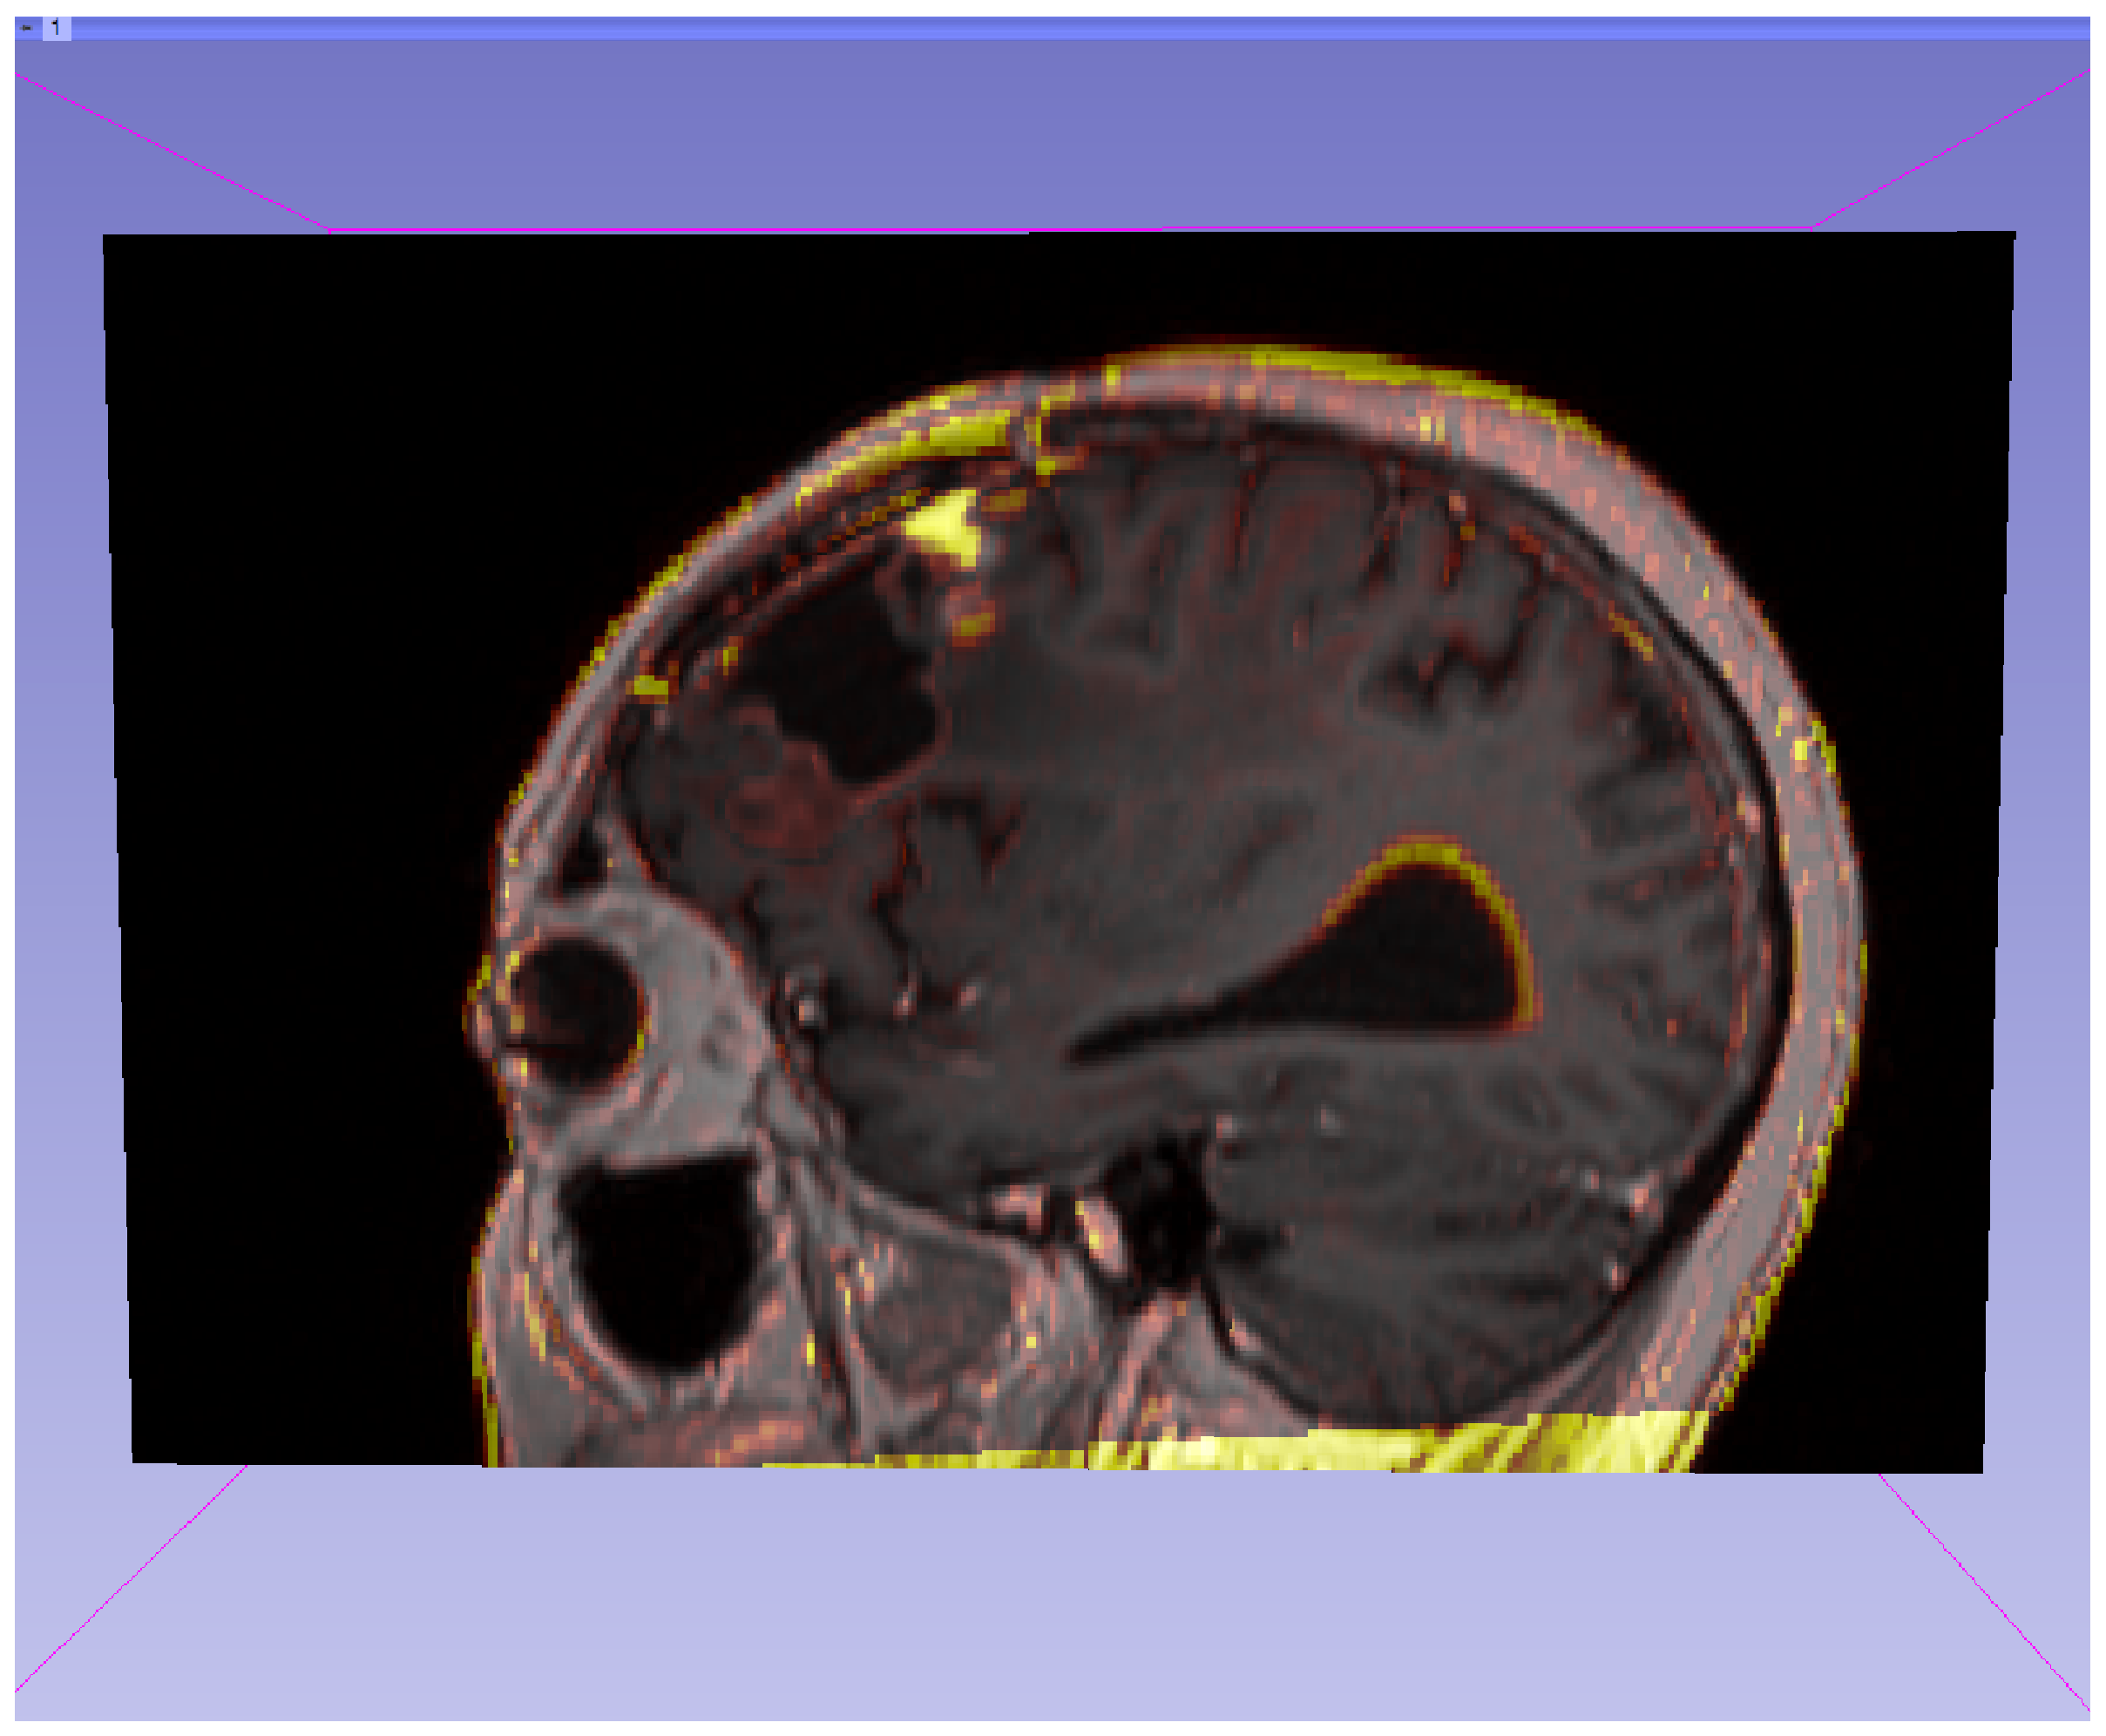
\includegraphics[scale=0.2]{/experiment_B2_P3/B2_Sagittal.eps}
  \caption{Voxel-based method. Patient 3: Sagittal plane}
  \label{B2_Sagittal}
\end{figure}


\subsubsection{Tensor-based Method}
This method also shows the expected difference due to the surgery
(correctly expressed as shrinkage, in green) which can be seen in the
images \ref{B2_TCoronal}, \ref{B2_TTraversal2} and \ref{B2_TSagittal}.

The image \ref{B2_TTraversal1} is showed for comparison with the
differences shown in image \ref{B2_Traversal1} in the previous
method. The tensor-based result doesn't show the exact same result;
however, some growth (in pink) can be seen. This could be attributed
to either inaccuracy of the method or to movement in the brain
consistent with the surgery.\\

Parameters used:
\begin{description}
\item \textit{Deformation field smoothing sigma:} 2.5
\item \textit{Shrinkage percentage:} 60
\item \textit{Growth percentage:} 50
\end{description}

\begin{figure}[H]
  \centering
  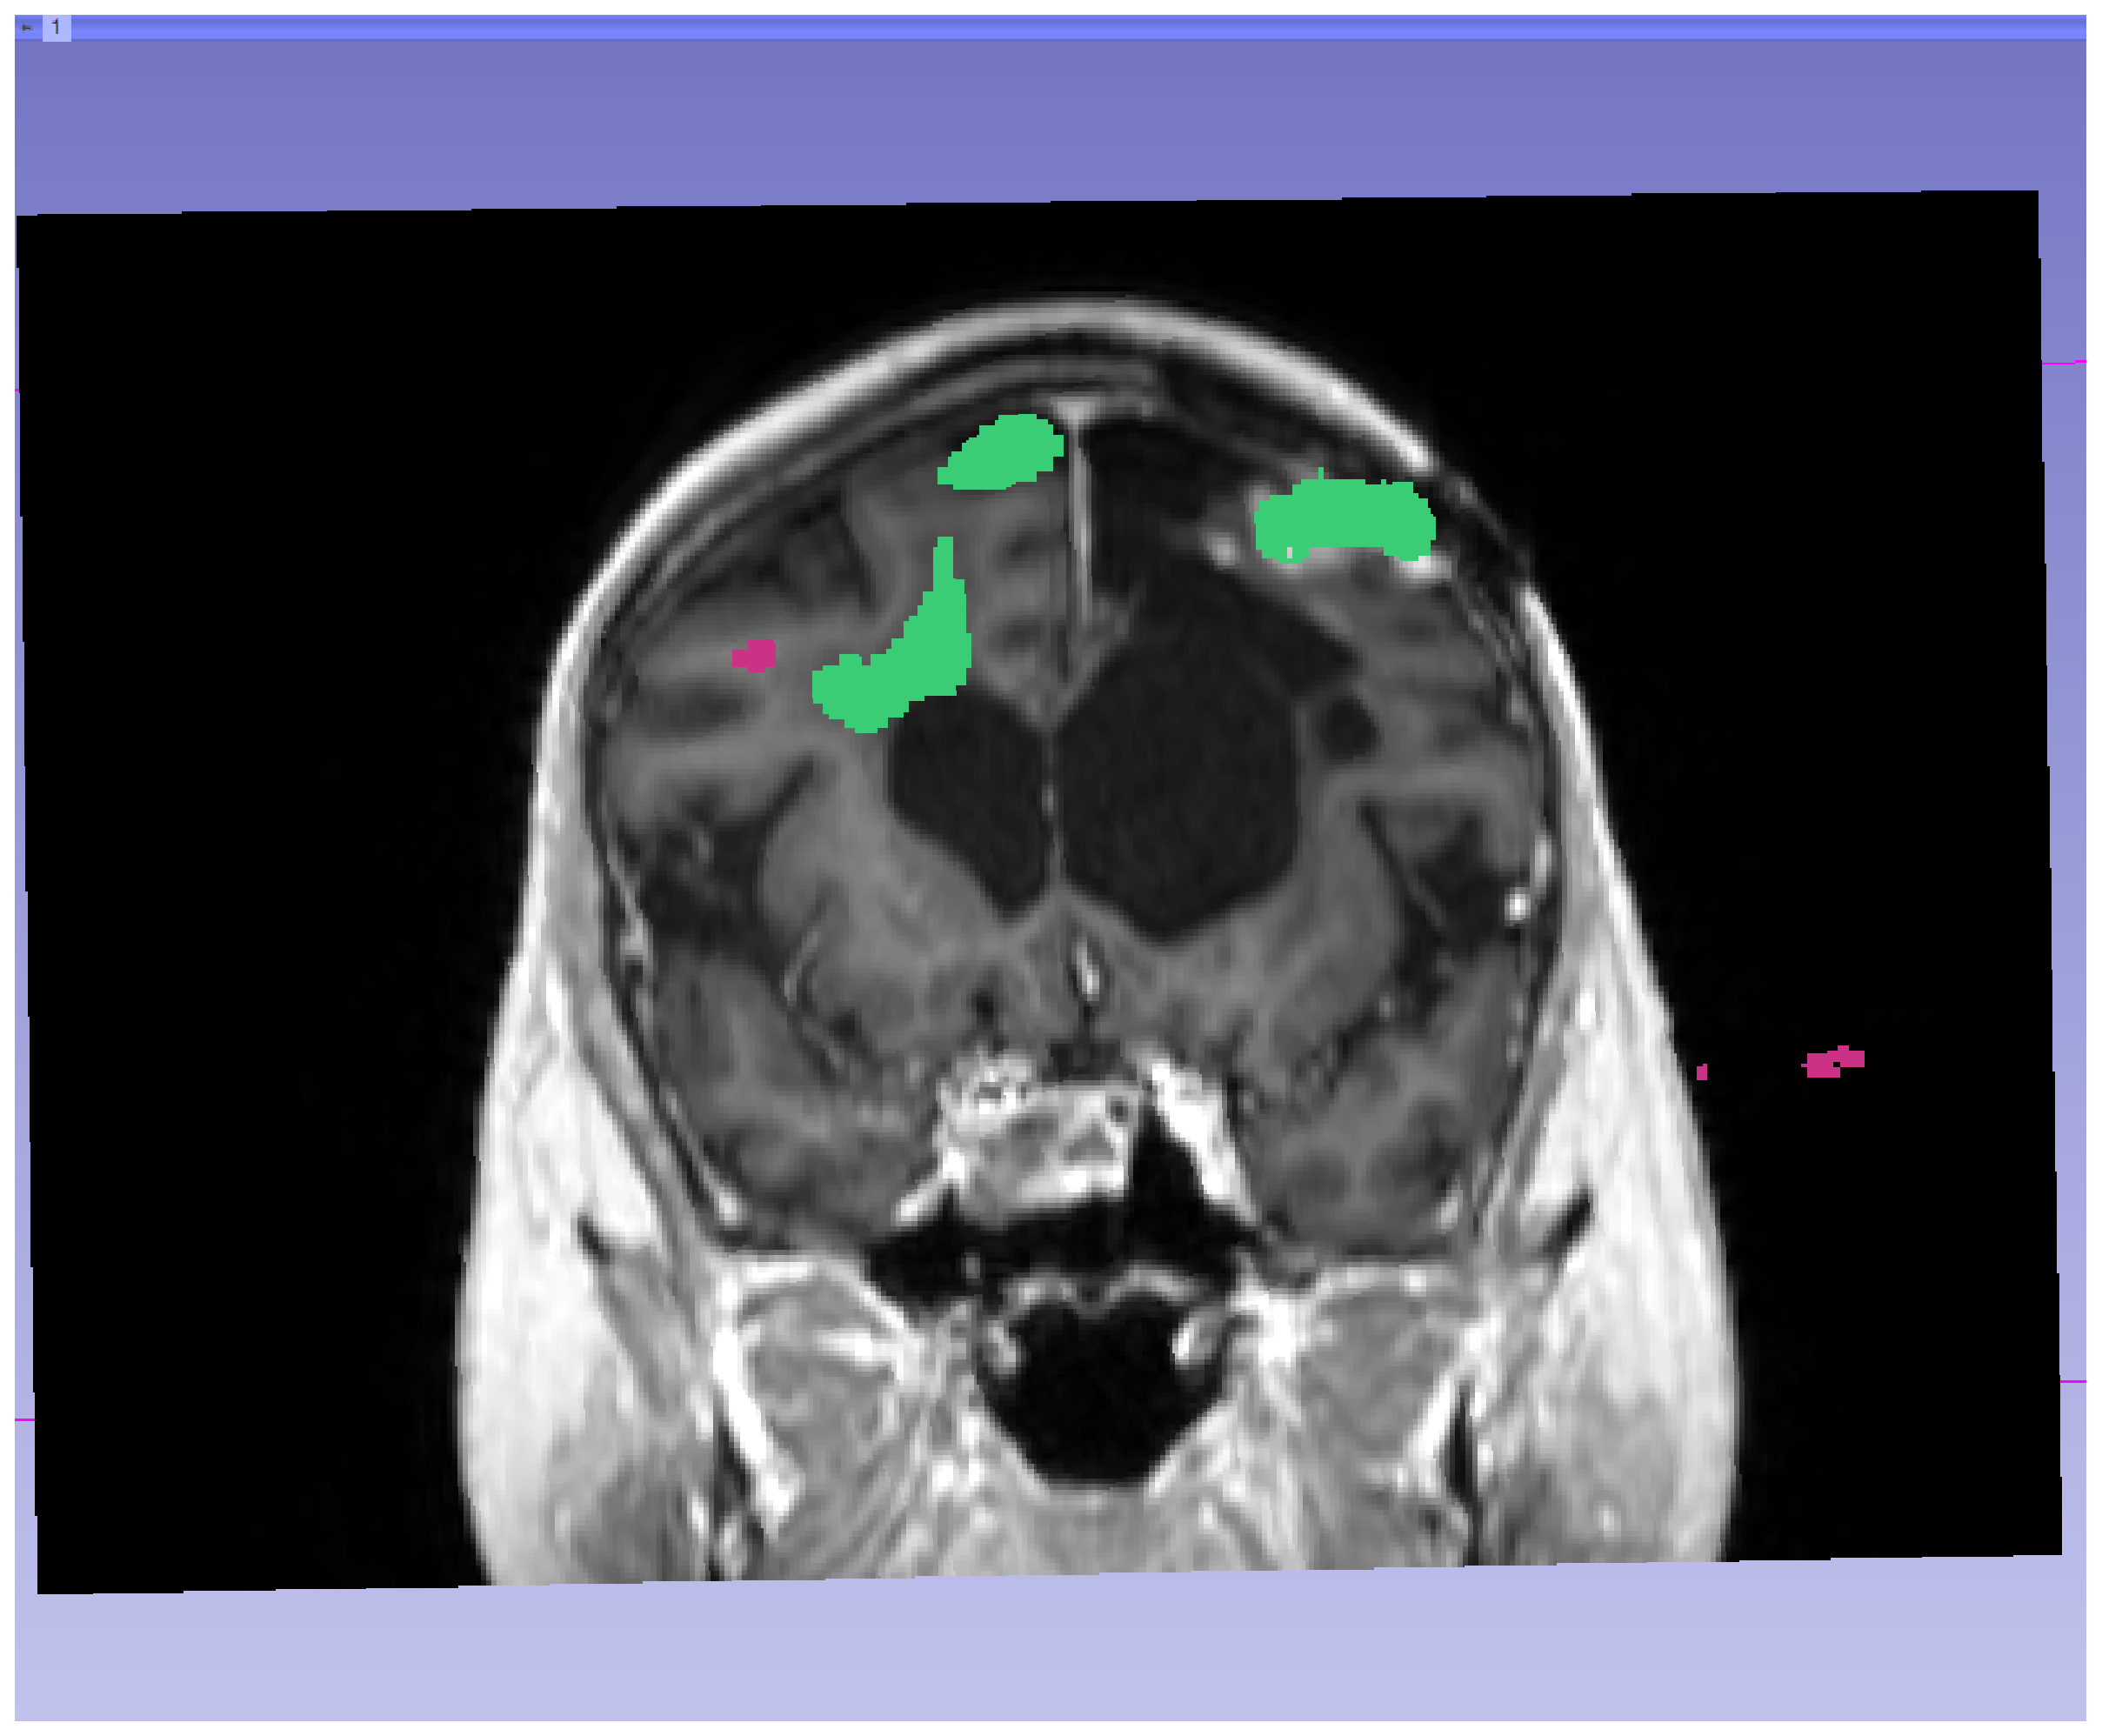
\includegraphics[scale=0.2]{/experiment_B2_P3/B2_Tensor_Coronal.eps}
  \caption{Tensor-based method. Patient 3: Coronal plane}
  \label{B2_TCoronal}
\end{figure}

\begin{figure}[H]
  \centering
  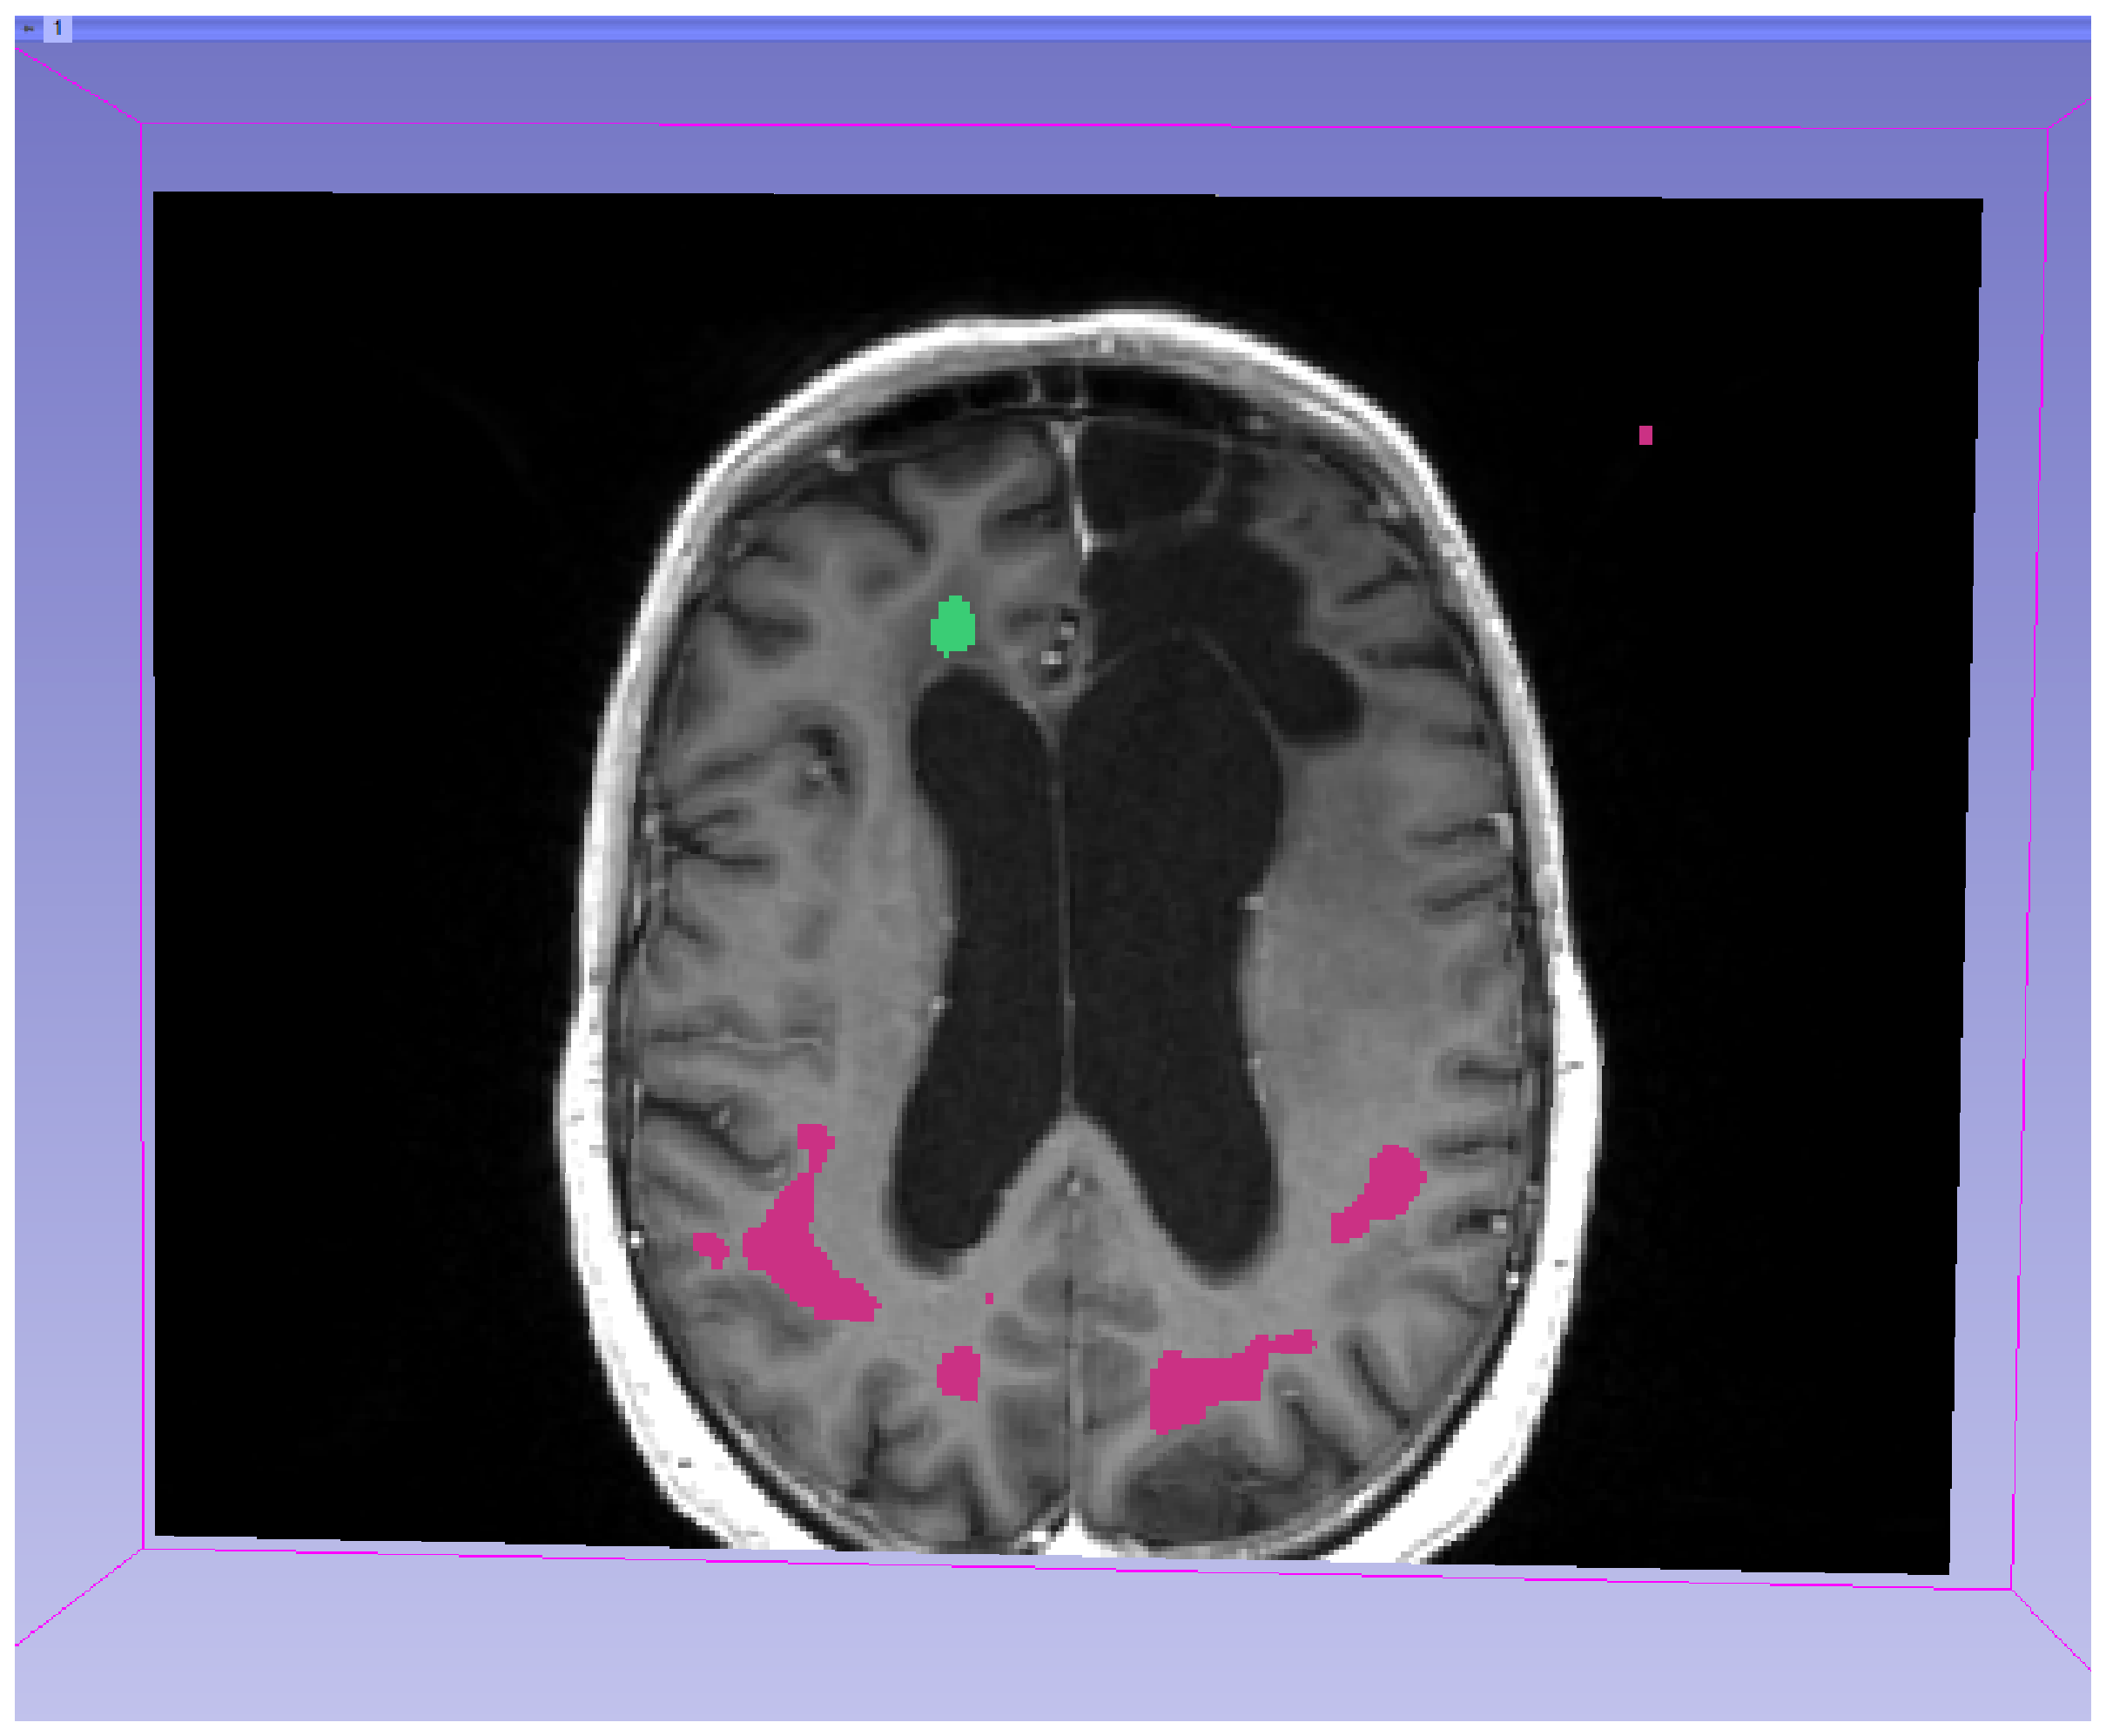
\includegraphics[scale=0.2]{/experiment_B2_P3/B2_Tensor_Traversal1.eps}
  \caption{Tensor-based method. Patient 3: Traversal plane}
  \label{B2_TTraversal1}
\end{figure}

\begin{figure}[H]
  \centering
  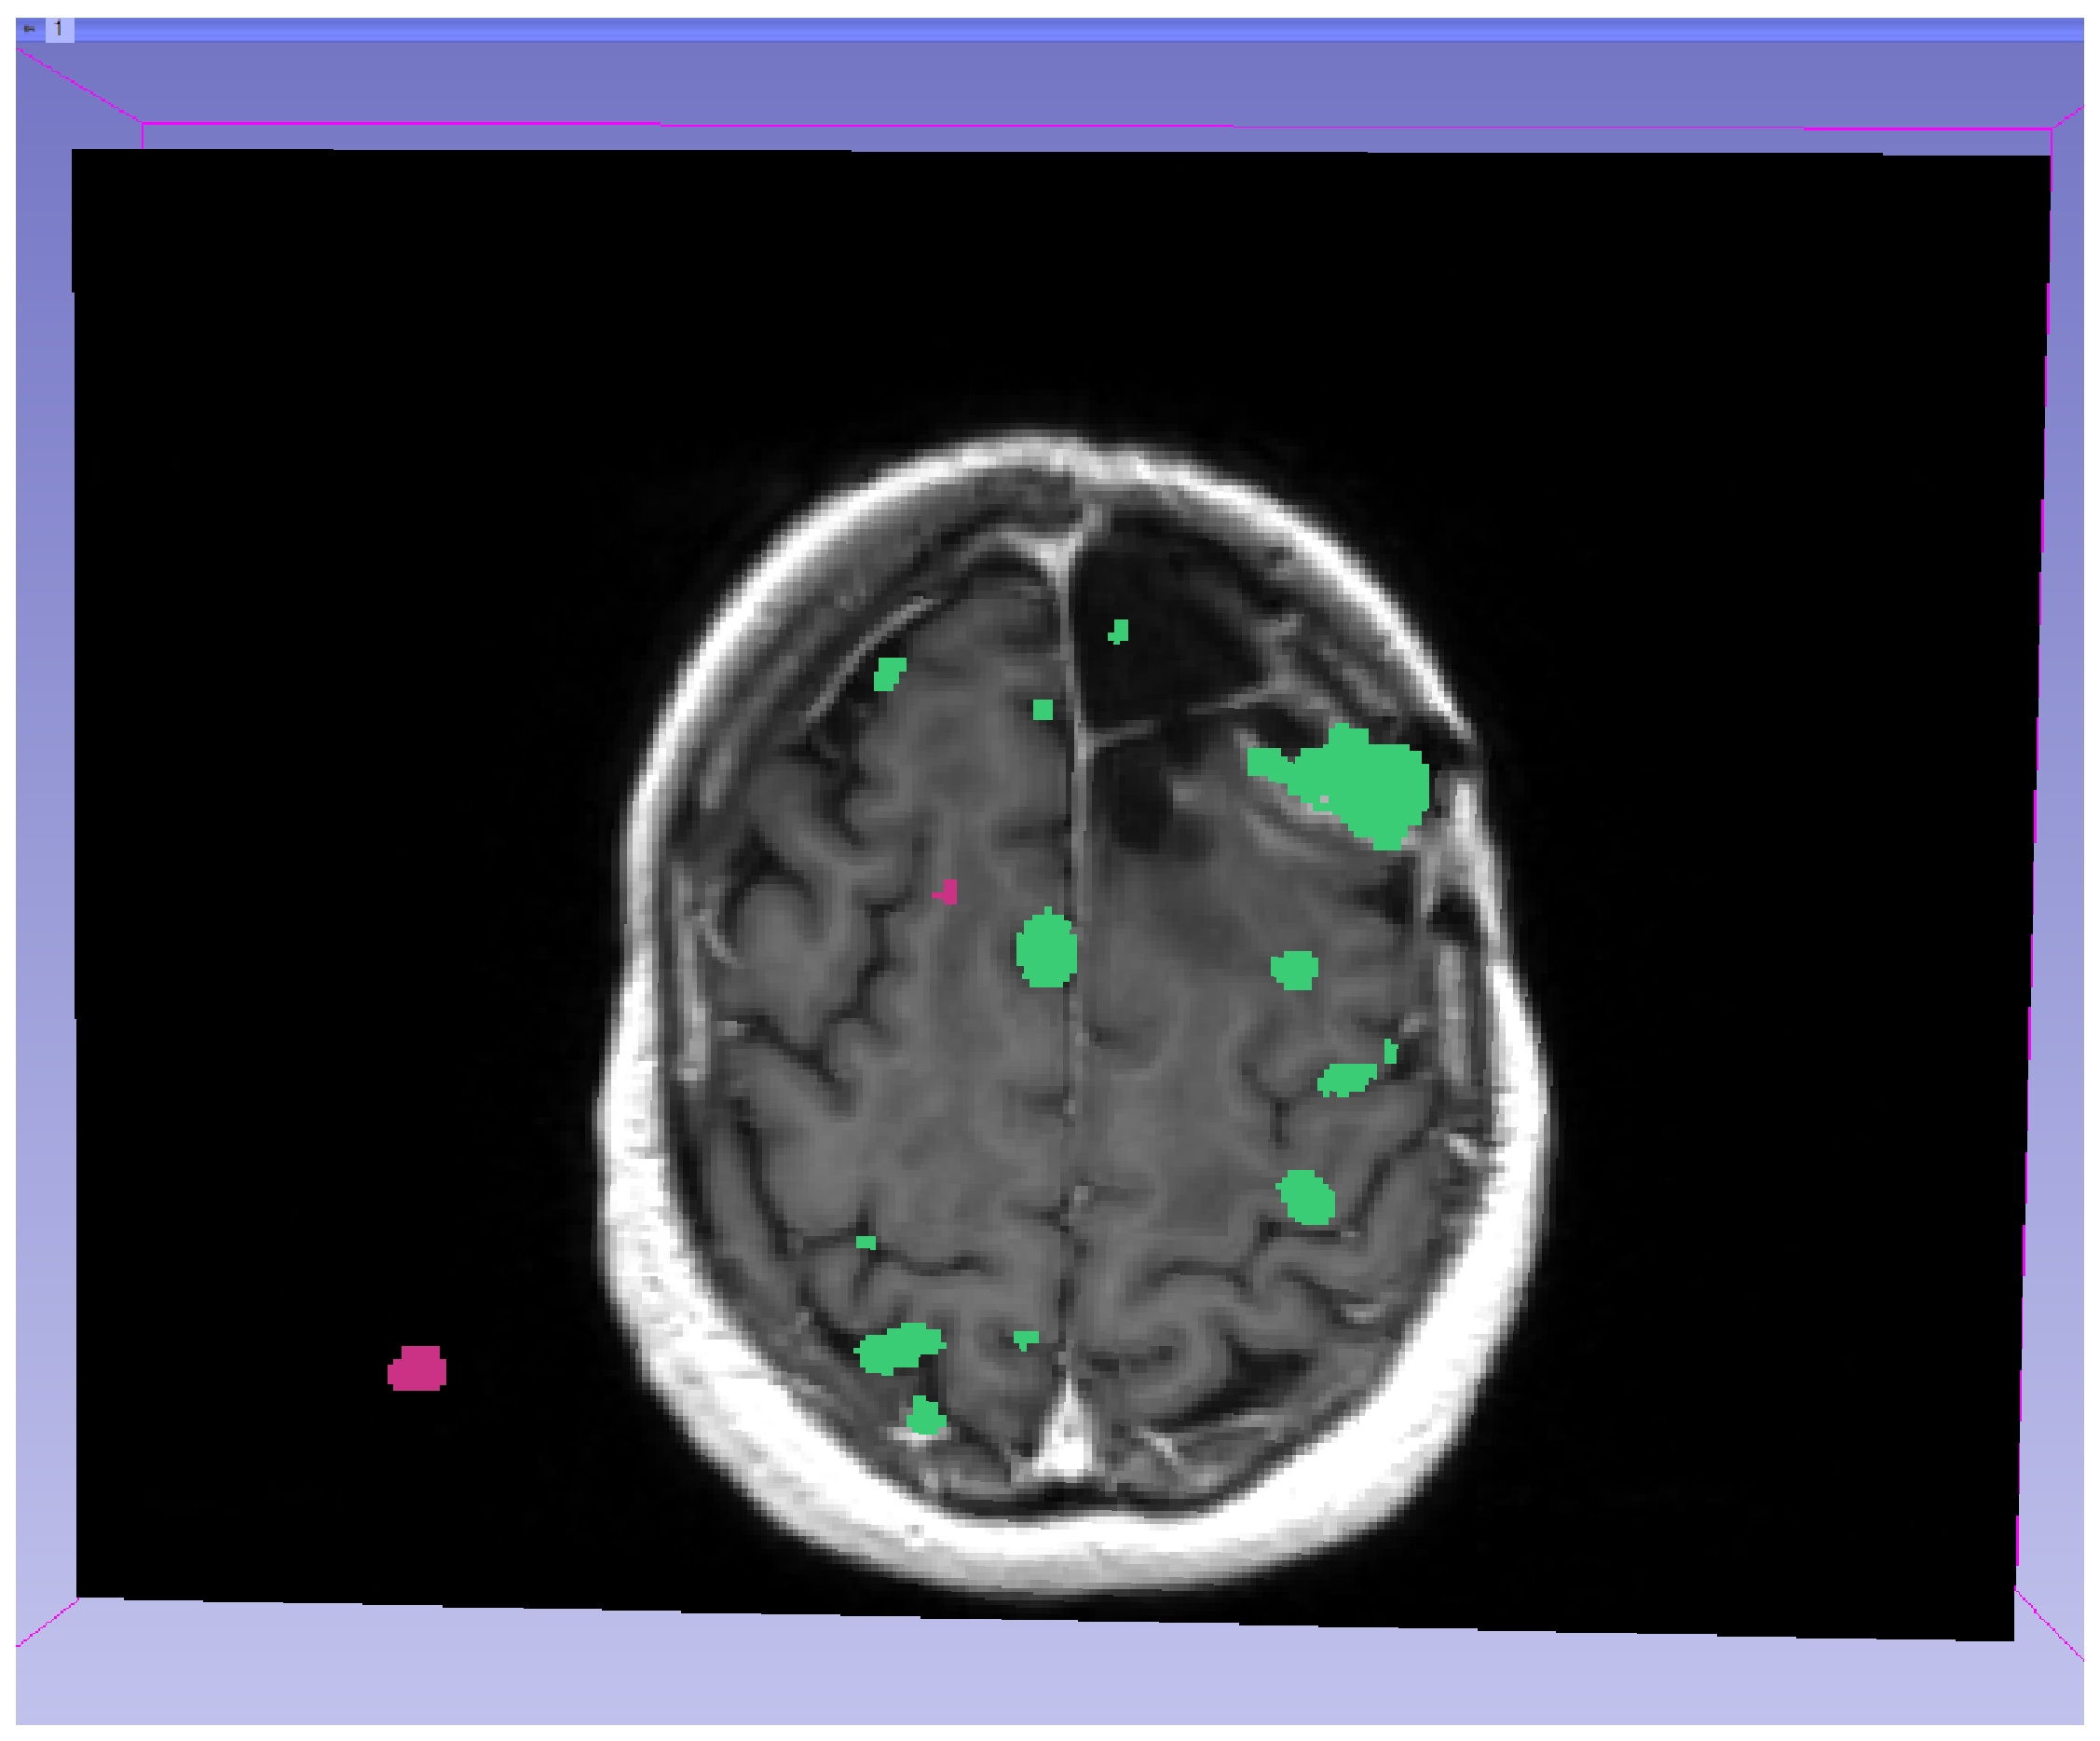
\includegraphics[scale=0.2]{/experiment_B2_P3/B2_Tensor_Traversal2.eps}
  \caption{Tensor-based method. Patient 3: Upper traversal plane}
  \label{B2_TTraversal2}
\end{figure}

\begin{figure}[H]
  \centering
  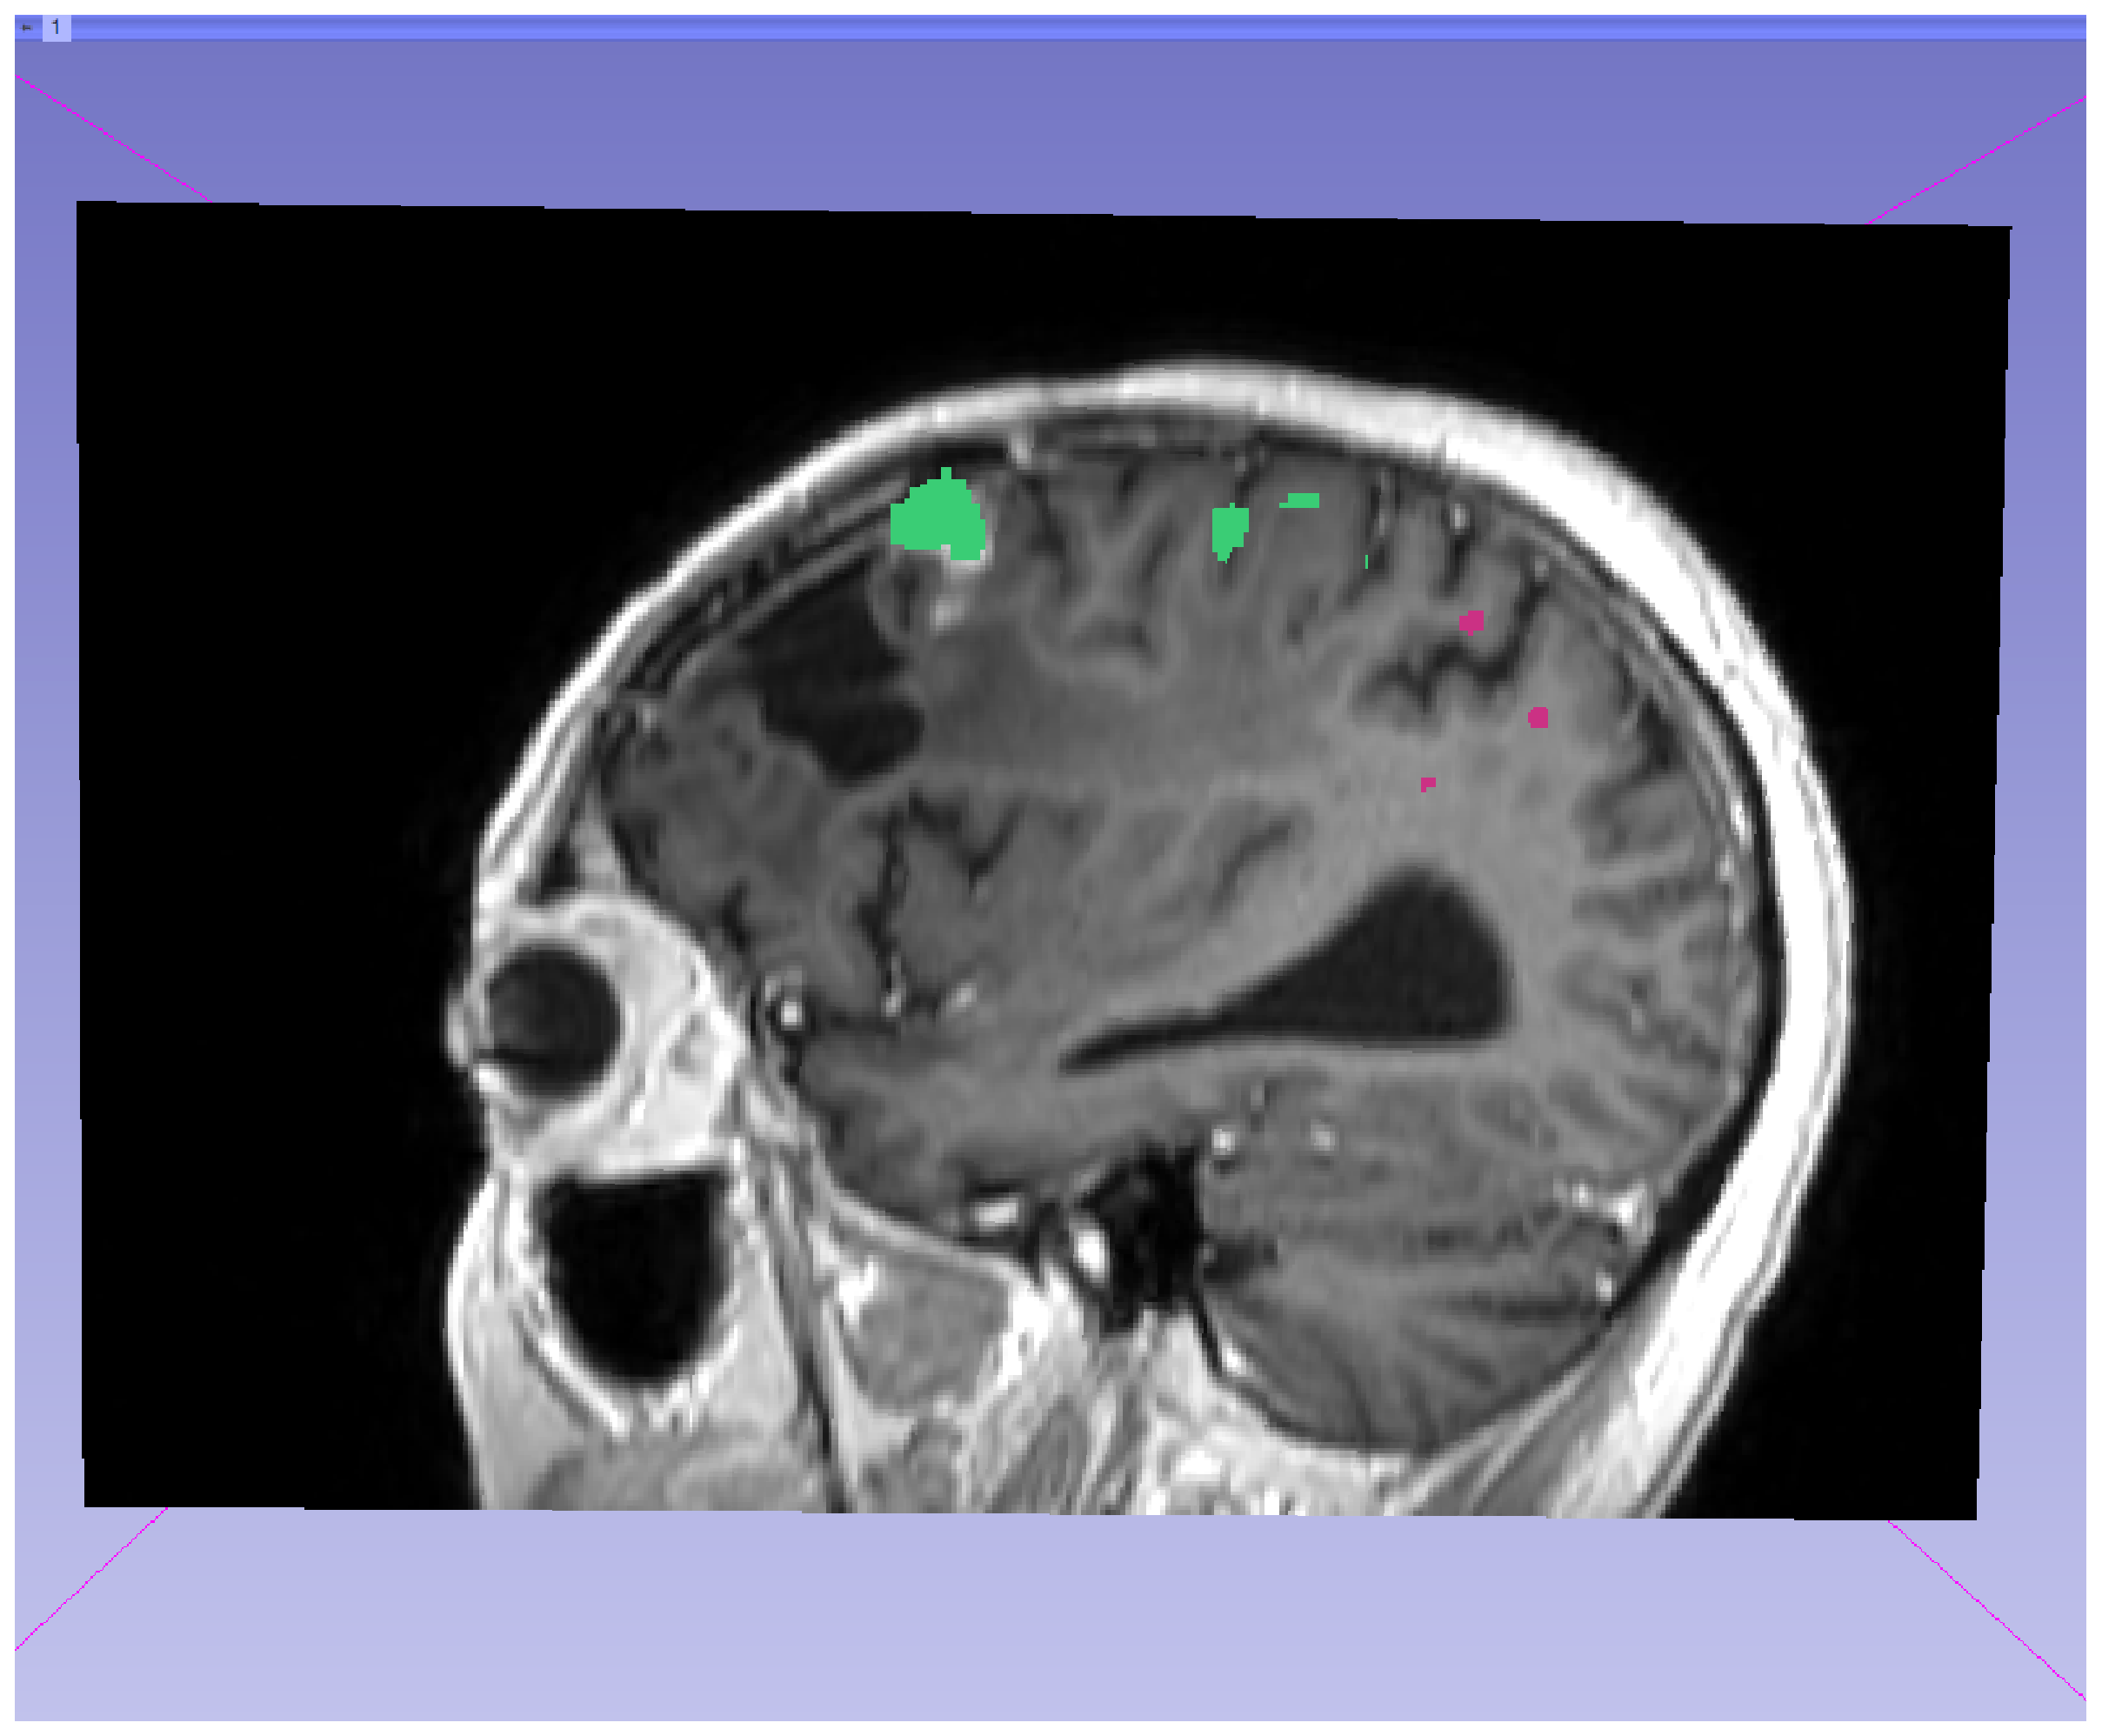
\includegraphics[scale=0.2]{/experiment_B2_P3/B2_Tensor_Sagittal.eps}
  \caption{Tensor-based method. Patient 3: Sagittal plane}
  \label{B2_TSagittal}
\end{figure}
     \chapter{Discussion}
This chapter contains an a analysis of the strenghts and weaknesses
of each of the proposed methods based on the results obtained after
several experiments with patient containing real and artificially
added differences.

\section{Voxel-based method}
This method performs especially well in cases of volume loss, since
this condition implies larger differences in intensity between both
volumes. According to the experiments performed, the size of this
differences can be really small and the method may still produce
useful results.\\

The method depends a lot on the registration results obtained in the
second step. If the registration result is poor, the program will
produce ``ghosts'' or false differences that may confuse the user.

Note that a poor registration result might not necessarily be a direct
consequence of the registration method chosen, it may also be due to
problems with the volumes; for example, if the patient's position
changes a lot from one volume to the next, or if the MRI machine has
very distinct settings in each examination.\\

Since in our specific case we deal with differences that are quite
small, sometimes it is still hard to see them in the results;
specially if we are looking at a screenshot of the application, rather
than the actual application where we can see all of the frames in the
volume.

\section{Tensor-based method}
This method has a lot of potential; since in theory, by using the
deformation field resulting from the registration, we have all the
information to be able to identify all the differences between the
volumes.\\

In spite of its potential, further analysis of the method results in
the following challenges:
\begin{enumerate}
\item We need to generate a ``useful'' deformation field; which in
  this case means a deformation field that is not too noisy, and from
  which we can obtain real differences.
\item We also need to figure out ``good values'' for the percentages
  of growth and shrinkage that we are going to use for the final
  result. This point is particularly complicated, since the
  \textit{Jacobian determinant} values are usually not distributed in
  the same way for different volumes.\\
\end{enumerate}

The module attempts to help the user find the right values by making
the most relevant numbers interactive in the user interface. However,
it is sometimes very hard to distinguish between actual differences
and noise caused by a non smooth deformation field.\\

Also, the \textit{Jacobian determinant} values are not regularly
distributed around zero; this means that in most cases, the range of
the values representing growth (located above zero), is much larger
that the range of values that represent shrinkage (values below
zero). As a consequence, the percentage of shrinkage is much more
sensitive to small changes than the percentage of growth.

     \chapter{Applications}

The original idea for the project came out of the necessity for a
program that could be used to find small differences between MRIs of
trauma patients at the Uppsala University Hospital.

The main doctor interested in the project is PhD. Raili Raininko, from
the Department of Radiology at the hospital, who collaborated with her
experience and comments during the entire course of this project.\\

So far, the application has been used in a study made with the
collaboration of the Department of Neuroscience of Uppsala University
and the Department of Radiology of the Uppsala University Hospital.

During the mentioned study, the MRIs of nineteen patients who
presented mild traumatic brain injuries where compared; with the first
MRI taken 2 or 3 days after the injury, and the second 3 to 7 months
after.

The application created during this project was used to corroborate
the results obtained after visual analysis of the MRIs by an expert
physician. 

The study concludes that loss of brain volume may be a
feasible marker of brain pathology after mild traumatic brain
injuries.\\

Volume comparison, and specifically medical image comparison,
continues to be a very challenging problem. The applications developed
during this project should be well received by the medical audience,
even if they do not guarantee a complete automatization of the
comparison process.

As described later on the \textit{Future Works} section, it would be
very useful to make the modules implemented available to the public by
making them a part of a new release of \textit{3D Slicer}.

In this way, the modules could be used, commented on, and even
possibly improved, by anyone who would be willing to use them or by a
member of the \textit{3D Slicer} developer community.


% TODO Joel project??
     \chapter{Conclusions}


\section{Future works}

- Improve Tensor-based method
- Make it public to Slicer people


\backmatter
    \nocite{*} % Remove this for your own citations
    \bibliographystyle{plain}
    \bibliography{References}

\end{document}